\chapter{Thực nghiệm và kết quả}
\label{Chapter4}
Chương này trình bày thiết kế thực nghiệm và các kết quả dùng để trả lời năm câu hỏi nghiên cứu của khóa luận. Cách tổ chức được xây dựng theo một chuỗi lập luận gồm khả năng chuyển giao trực tiếp của mô hình nền tảng, vai trò của hai phương thức đầu vào, hiệu năng theo điều kiện dữ liệu và chi phí, ảnh hưởng của từng thành phần, chất lượng biểu diễn đối với dữ liệu ngoài phân phối và mức phụ thuộc của dự đoán vào các nguồn thông tin. Các cấu hình có huấn luyện được đánh giá trên ba hạt giống 42, 123 và 456 với giá trị tổng hợp được báo cáo dưới dạng trung bình $\pm$ độ lệch chuẩn mẫu. Kết quả theo từng hạt giống và các phân tích bổ sung được trình bày tại Phụ lục~\ref{AppendixSeedResults}.

\section{Thiết kế thực nghiệm}
\label{sec:experimental_design}

\subsection{Chuẩn bị dữ liệu}
Nghiên cứu sử dụng bộ dữ liệu BTXRD \cite{Yao2025} được công bố và bộ dữ liệu CTCH được thu thập tại Bệnh viện Chấn thương Chỉnh hình Thành phố Hồ Chí Minh do giảng viên cung cấp. Các phần dưới đây mô tả nguồn gốc, cách thức thu thập và những số liệu thống kê liên quan đến từng bộ dữ liệu. Ngoài ra, cấu trúc thư mục và các bước tiền xử lý sẽ được mô tả ở Phụ lục~\ref{Appendix1}.

\subsubsection{Bộ dữ liệu BTXRD}
\label{subsec:btxrd-dataset}

BTXRD là bộ dữ liệu ảnh X-quang được xây dựng cho các bài toán phân lớp, định vị và phân vùng u xương nguyên phát. Phiên bản được sử dụng trong nghiên cứu gồm 3.746 ảnh, siêu dữ liệu về tuổi, giới tính, vị trí giải phẫu và tư thế chụp, cùng các chỉ báo về sự hiện diện, tính lành tính hoặc ác tính và phân nhóm tổn thương. Đối với 1.867 ảnh có u, bộ dữ liệu còn cung cấp tệp chú thích chứa thông tin vùng tổn thương.

Theo mô tả của bộ dữ liệu công bố, dữ liệu được tổng hợp từ ba bệnh viện tại Trung Quốc, Radiopaedia và MedPix. Dữ liệu bệnh viện được thu thập trong giai đoạn từ tháng 7 năm 2013 đến tháng 7 năm 2023, các chẩn đoán được xác nhận bằng mô bệnh học hoặc được hai bác sĩ X-quang thống nhất. Đối với hai nguồn trực tuyến, các ảnh liên quan đến u xương được hai chuyên gia tuyển chọn, đồng thời yêu cầu có thông tin tuổi và giới tính. Những vùng giải phẫu có ít mẫu hoặc nhiều nhiễu như đầu, cổ, ngực và bụng được loại bỏ, do đó phạm vi còn lại tập trung vào chi trên, chi dưới và xương chậu.

Quy trình chú thích được thực hiện bằng Labelme \cite{russell2008labelme}: một bác sĩ chuyên khoa u xương có 10 năm kinh nghiệm xác định vùng tổn thương, sau đó kết quả được một chuyên gia có 20 năm kinh nghiệm kiểm tra.

\paragraph{Đặc điểm dữ liệu và bài toán phân lớp}

Trong 3.746 mẫu, có 1.879 ảnh bình thường, 1.525 ảnh thuộc nhóm u lành tính và 342 ảnh thuộc nhóm u ác tính. Tuổi dao động từ 1 đến 88, gồm 2.098 mẫu nam và 1.648 mẫu nữ như được thể hiện trong Hình~\ref{fig:BTXRDinfo}.

Nhãn được thiết lập dưới dạng phân lớp đơn nhãn với 10 lớp. Nhãn bình thường được suy ra khi cờ chỉ báo u bằng 0, chín lớp còn lại được lấy từ các chỉ báo bệnh lý trong siêu dữ liệu. Bảng~\ref{tab:btxrd_splits} trình bày số lượng mẫu theo tập chia, trong khi Bảng~\ref{tab:btxrd_pathologies} trình bày phân bố lớp ở các tập chia.

\begin{figure}[H]
\centering
    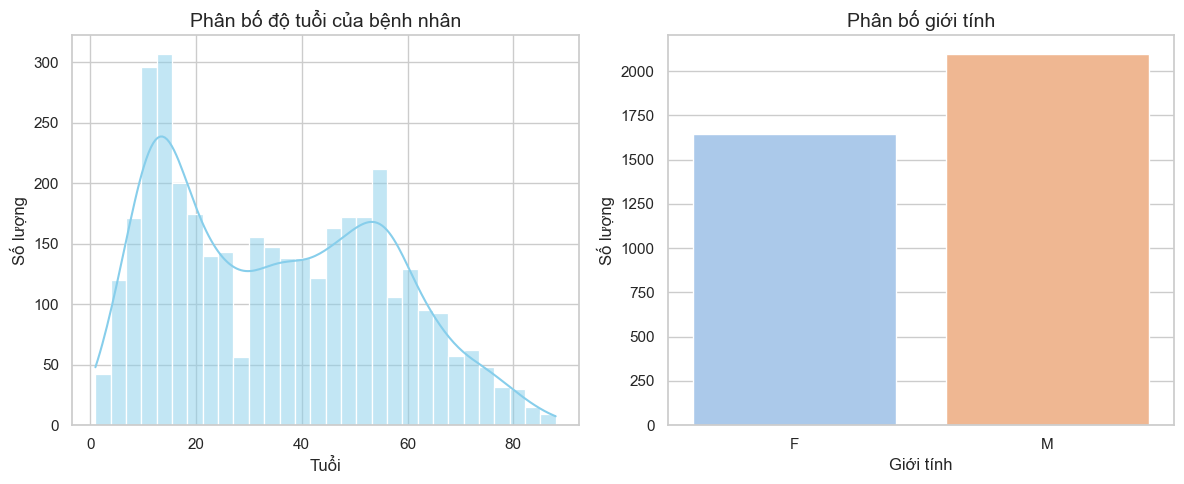
\includegraphics[width=1\linewidth]{images/BTXRDinfo.png}
    \caption{Phân bố độ tuổi và giới tính của các bệnh nhân được quan sát trong bộ dữ liệu BTXRD}
    \label{fig:BTXRDinfo}
\end{figure}

\begin{table}[htbp]
\centering
\small
\begin{tabular}{|l|c|c|}
\hline
\textbf{Tập chia} & \textbf{Số lượng hình ảnh} & \textbf{Tỷ lệ (\%)} \\ \hline
Huấn luyện & 2.621 & 70 \\ \hline
Xác thực & 375 & 10 \\ \hline
Kiểm thử & 750 & 20 \\ \hline
\textbf{Tổng cộng} & \textbf{3.746} & \textbf{100,00} \\ \hline
\end{tabular}%
\caption{Phân bổ mẫu theo các tập chia trong BTXRD}
\label{tab:btxrd_splits}
\end{table}

\begin{table}[htbp]
\centering
\small
\resizebox{\textwidth}{!}{%
\begin{tabular}{|l|r|r|r|r|r|}
\hline
\textbf{Nhãn bệnh lý} & \textbf{Huấn luyện} & \textbf{Xác thực} & \textbf{Kiểm thử} & \textbf{Tổng} & \textbf{Tỷ lệ} \\ \hline
Bình thường & 1.322 & 191 & 366 & 1.879 & 50,16\% \\ \hline
U xương sụn & 538 & 70 & 145 & 753 & 20,10\% \\ \hline
Sarcoma xương & 200 & 32 & 65 & 297 & 7,93\% \\ \hline
Đa u xương sụn & 189 & 29 & 45 & 263 & 7,02\% \\ \hline
Nang xương đơn thuần & 149 & 17 & 40 & 206 & 5,50\% \\ \hline
U lành tính khác & 83 & 8 & 24 & 115 & 3,07\% \\ \hline
U tế bào khổng lồ & 54 & 8 & 31 & 93 & 2,48\% \\ \hline
U sụn màng hoạt dịch & 35 & 7 & 9 & 51 & 1,36\% \\ \hline
U ác tính khác & 27 & 5 & 13 & 45 & 1,20\% \\ \hline
U xơ xương & 24 & 8 & 12 & 44 & 1,17\% \\ \hline
\textbf{Tổng} & \textbf{2.621} & \textbf{375} & \textbf{750} & \textbf{3.746} & \textbf{100,00\%} \\ \hline
\end{tabular}%
}
\caption{Phân bổ các lớp đơn nhãn sau chuẩn hóa trong bộ dữ liệu BTXRD}
\label{tab:btxrd_pathologies}
\end{table}

\clearpage

Bộ dữ liệu được chia ngẫu nhiên ở mức ảnh với hạt giống 42 và tỷ lệ 70/10/20 cho các tập huấn luyện, xác thực và kiểm thử. Tệp siêu dữ liệu không cung cấp mã người bệnh ổn định để nhóm các ảnh của cùng một ca trước khi chia. Vì vậy, kết quả BTXRD chỉ được diễn giải trong phạm vi phép chia ở mức ảnh.

Bộ dữ liệu BTXRD không cung cấp bệnh sử lâm sàng tương ứng với từng bệnh nhân. Do đó, để bổ sung nguồn văn bản đi kèm, nghiên cứu sử dụng quy trình sinh văn bản lâm sàng bằng siêu dữ liệu có sẵn được mô tả ở Phụ lục~\ref{AppendixBTXRD} và kết quả được minh họa như Bảng~\ref{tab:btxrd_example}.

\begin{table}[htbp]
\centering
\small
\resizebox{\textwidth}{!}{%
\begin{tabular}{|C{1.8cm}|C{1.8cm}|L{10.5cm}|}
\hline
\textbf{Ảnh} & \textbf{Nhãn} & \textbf{Văn bản giả lâm sàng được sinh} \\ \hline
\adjustbox{valign=c}{\includegraphics[width=1.7cm,height=4.5cm,keepaspectratio]{../../data/BTXRD/images/IMG000001.jpeg}}
&
\textit{other mt}
&
Patient: 48-year-old female. Reason for admission: Pain and swelling of the hip bone. Disease history: Pain in the hip bone for 1 month; associated with decreased appetite. Physical examination: Palpable mass; tenderness on palpation; mild swelling. Personal medical history: No prior bone disease or fracture. No relevant surgical or medical history. Radiographic evaluation: AP view of the hip bone was obtained.
\\ \hline
\adjustbox{valign=c}{\includegraphics[width=1.7cm,height=4.5cm,keepaspectratio]{../../data/BTXRD/images/IMG000014.jpeg}}
&
\textit{multiple osteochondromas}
&
Patient: 64-year-old male. Reason for admission: Progressive pain in the humerus. Disease history: The patient reports worsening pain in the humerus for 1 month. Physical examination: Palpable mass with local tenderness; no lymphadenopathy detected. Personal medical history: No prior bone disease or fracture. History of age-related degenerative changes; no prior bone lesions. Radiographic evaluation: AP view of the humerus was obtained.
\\ \hline
\end{tabular}%
}
\caption{Ví dụ ảnh, nhãn và văn bản giả lâm sàng được sinh của bộ dữ liệu BTXRD}
\label{tab:btxrd_example}
\end{table}

Trong thiết kế thực nghiệm, BTXRD được sử dụng để khảo sát khả năng chuyển giao sang bài toán u xương, ảnh hưởng của mất cân bằng lớp và hành vi của mô hình trong thiết lập văn bản tổng hợp. Do văn bản lâm sàng được sinh từ siêu dữ liệu và chịu ảnh hưởng của các cờ nhóm bệnh, kết quả trên bộ dữ liệu này không được diễn giải tương đương với kết quả thu được từ bệnh sử lâm sàng thực tế.

\subsubsection{Bộ dữ liệu CTCH}
\label{subsec:ctch-dataset}

CTCH là bộ dữ liệu X-quang xương được thu thập tại Bệnh viện Chấn thương Chỉnh hình Thành phố Hồ Chí Minh và được giảng viên Võ Thế Hào cùng giảng viên Đỗ Phúc Thịnh cung cấp cho nghiên cứu. Dữ liệu nguồn gồm ảnh được lựa chọn từ từng ca khám và các trường bệnh án tiếng Việt liên quan đến lý do vào viện, diễn tiến bệnh, tiền sử, kết quả khảo sát hình ảnh và chẩn đoán chuyên môn. Văn bản đầu vào chỉ sử dụng lý do vào viện, diễn tiến bệnh và tiền sử. Kết quả khảo sát hình ảnh, chẩn đoán chuyên môn và nhãn không được đưa vào chuỗi văn bản. Phạm vi thực nghiệm chỉ sử dụng ảnh X-quang đại diện cho vị trí bệnh lý. Ảnh từ phương thức tạo ảnh khác hoặc không đại diện cho vị trí bệnh lý không được đưa vào tập phân lớp. Quy trình lựa chọn trường và kiểm soát rò rỉ nhãn được trình bày tại Phụ lục~\ref{AppendixCTCH}.

\paragraph{Đạo đức nghiên cứu, quyền riêng tư và tính sẵn có của dữ liệu}

Bộ dữ liệu được sử dụng theo thỏa thuận bảo mật đã ký kết và chỉ phục vụ mục đích nghiên cứu. Trước khi xử lý, các thông tin có khả năng định danh trực tiếp người bệnh đã được loại bỏ và các mã hồ sơ chỉ được dùng để liên kết dữ liệu, kiểm soát việc phân chia tập và không được công bố trong kết quả nghiên cứu. 

Do chứa thông tin y tế nhạy cảm, bộ dữ liệu gốc không được công khai và khóa luận chỉ trình bày số liệu thống kê cùng kết quả tổng hợp. Mọi hoạt động kiểm định hoặc triển khai trong môi trường lâm sàng về sau cần tuân thủ quy định bảo vệ dữ liệu và được cơ quan có thẩm quyền phê duyệt.

\paragraph{Đặc điểm dữ liệu và bài toán phân lớp}

Việc chia dữ liệu được thực hiện theo người bệnh với hạt giống ngẫu nhiên 42 và tỷ lệ mục tiêu 70/10/20. Người bệnh được nhóm theo lớp chính trước khi phân bổ để duy trì sự hiện diện của các lớp ít mẫu ở cả ba tập khi số lượng cho phép. Kết quả như được thể hiện ở Bảng~\ref{tab:ctch_splits} gồm 2.265 mẫu huấn luyện, 315 mẫu xác thực và 669 mẫu kiểm thử và Bảng~\ref{tab:ctch_pathologies} thể hiện chi tiết số lượng mẫu trong từng lớp trong các tập chia.

\clearpage

\begin{table}[htbp]
\centering
\small
\begin{tabular}{|l|r|r|}
\hline
\textbf{Tập dữ liệu} & \textbf{Số lượng ảnh} & \textbf{Tỷ lệ} \\ \hline
Huấn luyện & 2.265 & 69,71\% \\ \hline
Xác thực & 315 & 9,70\% \\ \hline
Kiểm thử & 669 & 20,59\% \\ \hline
\textbf{Tổng cộng} & \textbf{3.249} & \textbf{100,00\%} \\ \hline
\end{tabular}%
\caption{Phân bổ mẫu trong phân phối của CTCH theo tập dữ liệu}
\label{tab:ctch_splits}
\end{table}

\begin{table}[htbp]
\centering
\small
\resizebox{\textwidth}{!}{%
\begin{tabular}{|l|r|r|r|r|r|}
\hline
\textbf{Lớp} & \textbf{Huấn luyện} & \textbf{Xác thực} & \textbf{Kiểm thử} & \textbf{Tổng} & \textbf{Tỷ lệ} \\ \hline
Bình thường & 760 & 108 & 218 & 1.086 & 33,43\% \\ \hline
Gãy xương quay & 209 & 29 & 61 & 299 & 9,20\% \\ \hline
Gãy xương cánh tay & 147 & 21 & 42 & 210 & 6,46\% \\ \hline
Gãy xương đùi & 106 & 15 & 31 & 152 & 4,68\% \\ \hline
Gãy xương ngón tay & 102 & 14 & 31 & 147 & 4,52\% \\ \hline
Gãy xương chày & 99 & 14 & 29 & 142 & 4,37\% \\ \hline
Gãy xương cẳng tay & 99 & 14 & 29 & 142 & 4,37\% \\ \hline
Gãy xương cổ chân & 87 & 12 & 26 & 125 & 3,85\% \\ \hline
Gãy xương cẳng chân & 85 & 12 & 25 & 122 & 3,76\% \\ \hline
Gãy xương vùng vai & 70 & 10 & 21 & 101 & 3,11\% \\ \hline
Gãy xương bàn chân & 68 & 9 & 21 & 98 & 3,02\% \\ \hline
Gãy cột sống thắt lưng & 53 & 7 & 16 & 76 & 2,34\% \\ \hline
Gãy xương bàn tay & 53 & 7 & 16 & 76 & 2,34\% \\ \hline
Gãy xương ngón chân & 52 & 7 & 16 & 75 & 2,31\% \\ \hline
Viêm khớp & 47 & 6 & 15 & 68 & 2,09\% \\ \hline
Gãy xương trụ & 46 & 6 & 14 & 66 & 2,03\% \\ \hline
Cắt cụt ngón tay & 42 & 6 & 13 & 61 & 1,88\% \\ \hline
Gãy xương bánh chè & 41 & 5 & 13 & 59 & 1,82\% \\ \hline
Gãy xương gót & 36 & 5 & 11 & 52 & 1,60\% \\ \hline
Gãy cột sống ngực & 28 & 4 & 8 & 40 & 1,23\% \\ \hline
Gãy xương thuyền & 19 & 2 & 7 & 28 & 0,86\% \\ \hline
Gãy xương vùng chậu & 16 & 2 & 6 & 24 & 0,74\% \\ \hline
\textbf{Tổng cộng} & \textbf{2.265} & \textbf{315} & \textbf{669} & \textbf{3.249} & \textbf{100,00\%} \\ \hline
\end{tabular}%
}
\caption{Phân bố 22 lớp của CTCH trong ba tập dữ liệu}
\label{tab:ctch_pathologies}
\end{table}

Mỗi hồ sơ được liên kết với một ảnh X-quang duy nhất. Trong quần thể phân lớp hiện tại, 3.249 ảnh tương ứng với 3.249 mã bệnh nhân và quần thể ngoài phân phối gồm 44 ảnh từ 44 mã khác, không giao với quần thể phân lớp. Bảng~\ref{tab:ctch_example} minh họa một số mẫu sau tiền xử lý. Quy trình sàng lọc, lựa chọn trường văn bản và kiểm tra toàn vẹn được mô tả tại Phụ lục~\ref{AppendixCTCH}.

Các mẫu ngoài phân phối không được đưa vào huấn luyện, xác thực hoặc kiểm thử bộ phân lớp 22 lớp. Trong 44 mẫu này, 34 mẫu thuộc nhóm chấn thương và 10 mẫu thuộc nhóm viêm nhiễm nhưng biểu hiện bệnh lý nằm ngoài không gian nhãn đích. Do đó, chúng chỉ được sử dụng trong kịch bản đánh giá dữ liệu ngoài phân phối được trình bày ở phần thực nghiệm.


\begin{table}[htbp]
\centering
\small
\resizebox{\textwidth}{!}{%
\begin{tabular}{|C{1.8cm}|C{1.8cm}|L{10.5cm}|}
\hline
\textbf{Ảnh} & \textbf{Nhãn} & \textbf{Bệnh sử lâm sàng} \\ \hline
\adjustbox{valign=c}{\includegraphics[width=1.7cm,height=4.5cm,keepaspectratio]{../../data/CTCH/images/153_img-86413-00001.jpg}}
&
\textit{Lower leg fracture}
&
Reason for admission: Right lower leg pain. Disease history: The patient fell from the roof at 3:00 p.m. on October 17, 2024 in Tien Giang; no first aid. to the Orthopedic Trauma Hospital. Personal medical history: Nasopharynx is being treated
\\ \hline
\adjustbox{valign=c}{\includegraphics[width=1.7cm,height=4.5cm,keepaspectratio]{../../data/CTCH/images/118_img-03248-00001.jpg}}
&
\textit{Finger phalanx fracture}
&
Reason for admission: Right hand wound. Disease history: The patient had his right hand cut by a saw at 2:00 p.m. on October 17, 2024 in Dong Nai; Go to the local medical station for first aid. to the Orthopedic Trauma Hospital. Personal medical history: Right hand third metatarsal fusion surgery 9 years ago
\\ \hline
\end{tabular}%
}
\caption{Các ví dụ ảnh, nhãn và bệnh sử lâm sàng của bộ dữ liệu CTCH}
\label{tab:ctch_example}
\end{table}

CTCH được xem là nguồn bằng chứng chính cho câu hỏi về giá trị của học đa phương thức, vì mỗi ảnh được liên kết với bệnh sử lâm sàng có sẵn và phép chia được thực hiện theo người bệnh. Bộ dữ liệu này đồng thời cung cấp quần thể ngoài không gian nhãn để khảo sát cảnh báo dữ liệu ngoài phân phối và toàn bộ 669 mẫu kiểm thử được dùng cho phân tích nguồn thông tin của dự đoán.


\subsection{Nội dung thực nghiệm}
\label{sec:experiment_content}
Các thực nghiệm được tổ chức theo năm câu hỏi nghiên cứu như đã trình bày ở Chương~\ref{Chapter1}. Bảng~\ref{tab:research_question_mapping} trình bày giả thuyết cần kiểm tra, thực nghiệm chính và độ đo được ưu tiên trong quá trình diễn giải. Điểm F1 trung bình theo lớp là độ đo phân lớp chính vì hai bộ dữ liệu đều mất cân bằng. Các độ đo xếp hạng, hiệu chỉnh, cảnh báo dữ liệu ngoài phân phối và chi phí được dùng để làm rõ những đánh đổi mà một độ đo đơn lẻ không phản ánh đầy đủ.

\begin{table}[htbp]
\centering
\resizebox{\columnwidth}{!}{%
\begin{tabular}{|l|l|l|l|}
\hline
\multicolumn{1}{|c|}{\textbf{\begin{tabular}[c]{@{}c@{}}Câu hỏi \\ nghiên cứu\end{tabular}}} &
  \multicolumn{1}{c|}{\textbf{Giả thuyết kiểm tra}} &
  \multicolumn{1}{c|}{\textbf{Thực nghiệm chính}} &
  \multicolumn{1}{c|}{\textbf{Độ đo chính}} \\ \hline
\begin{tabular}[c]{@{}l@{}}Vai trò của ảnh \\ và văn bản\end{tabular} &
  \begin{tabular}[c]{@{}l@{}}Ảnh X-quang và văn bản đi kèm \\ cung cấp thông tin bổ sung. Việc \\ làm sai quan hệ ghép cặp sẽ làm \\ suy giảm dự đoán.\end{tabular} &
  \begin{tabular}[c]{@{}l@{}}So sánh ảnh-văn bản, chỉ ảnh, \\ chỉ văn bản và văn bản ghép \\ khác lớp trên CTCH và BTXRD.\end{tabular} &
  \begin{tabular}[c]{@{}l@{}}Điểm F1 trung bình \\ theo lớp và độ chính \\ xác cân bằng.\end{tabular} \\ \hline
\begin{tabular}[c]{@{}l@{}}Đóng góp của \\ các thành phần\end{tabular} &
  \begin{tabular}[c]{@{}l@{}}Nhánh ảnh cục bộ, huấn luyện \\ hai pha, dung hợp và đầu tâm \\ lớp tác động khác nhau đến \\ quyết định lớp, chất lượng xếp \\ hạng và hiệu chỉnh.\end{tabular} &
  \begin{tabular}[c]{@{}l@{}}Loại bỏ từng thành phần và \\ đối chứng theo nhóm mã hóa \\ ảnh, huấn luyện, dung hợp, \\ đầu phân lớp và mức thích \\ nghi bộ mã hóa.\end{tabular} &
  \begin{tabular}[c]{@{}l@{}}Điểm F1 trung bình \\ theo lớp, diện tích dưới \\ hai đường cong xếp hạng \\ và sai số hiệu chỉnh kỳ vọng.\end{tabular} \\ \hline
\begin{tabular}[c]{@{}l@{}}Đánh đổi dữ liệu, \\ tham số và chi phí\end{tabular} &
  \begin{tabular}[c]{@{}l@{}}XBone-Net và chiến lược LoRA \\ duy trì hiệu năng cạnh tranh khi \\ dữ liệu hạn chế và giảm số tham \\ số cần cập nhật, nhưng không nhất \\ thiết giảm chi phí suy luận.\end{tabular} &
  \begin{tabular}[c]{@{}l@{}}So sánh không mẫu, 1, 10, 20 \\ mẫu mỗi lớp và toàn bộ dữ liệu, \\ đồng thời đo tham số, thời gian, \\ thông lượng, độ trễ và số phép toán.\end{tabular} &
  \begin{tabular}[c]{@{}l@{}}Điểm F1 trung bình theo \\ lớp, số tham số cập nhật, \\ thông lượng và độ trễ.\end{tabular} \\ \hline
\begin{tabular}[c]{@{}l@{}}Phân biệt dữ liệu \\ ngoài phân phối\end{tabular} &
  \begin{tabular}[c]{@{}l@{}}Không gian biểu diễn chứa tín \\ hiệu giúp tách mẫu trong phân \\ phối khỏi mẫu ngoài không gian \\ nhãn và mẫu khác bộ dữ liệu.\end{tabular} &
  \begin{tabular}[c]{@{}l@{}}So sánh điểm cosine theo tâm lớp, \\ Mahalanobis, láng giềng gần nhất \\ và entropy trên hai kịch bản dịch \\ chuyển.\end{tabular} &
  \begin{tabular}[c]{@{}l@{}}Diện tích dưới đường cong \\ phân biệt và FPR@95\%TPR.\end{tabular} \\ \hline
\begin{tabular}[c]{@{}l@{}}Nguồn thông \\ tin của dự đoán\end{tabular} &
  \begin{tabular}[c]{@{}l@{}}Ảnh toàn cục, các đơn vị ảnh cục \\ bộ và bệnh sử có mức ảnh hưởng \\ khác nhau. Thứ tự quy đóng cần \\ làm xác suất lớp đích giảm nhanh \\ hơn đối chứng ngẫu nhiên.\end{tabular} &
  \begin{tabular}[c]{@{}l@{}}Can thiệp từng nguồn, tích phân \\ gradient, kiểm tra loại bỏ--khôi \\ phục và phân tích trường hợp \\ đúng, sai.\end{tabular} &
  \begin{tabular}[c]{@{}l@{}}Mức giảm xác suất lớp đích, \\ diện tích dưới đường cong \\ loại bỏ và chênh lệch so với \\ thứ tự ngẫu nhiên.\end{tabular} \\ \hline
\end{tabular}%
}
\caption{Ánh xạ câu hỏi nghiên cứu với giả thuyết, thực nghiệm và độ đo chính}
\label{tab:research_question_mapping}
\end{table}

Ở thiết lập không mẫu, CLIP, MedCLIP, PubMedCLIP và BiomedCLIP được giữ cố định, còn tên lớp tiếng Anh được thay vào câu nhắc \cite{CLIP}:
\begin{quote}
\small\raggedright\ttfamily
A radiograph showing [tên lớp].
\end{quote}
Biểu diễn ảnh và câu nhắc được chuẩn hóa rồi so sánh bằng độ tương đồng cosine. Thiết lập này chỉ đóng vai trò mốc chuyển giao trực tiếp. Trong trường hợp mẫu học hạn chế, tối đa 1, 10 hoặc 20 mẫu mỗi lớp được lấy không hoàn lại theo từng hạt giống, trong khi tập xác thực và tập kiểm thử được giữ nguyên. CTCH chỉ có 19 mẫu gãy xương thuyền và 16 mẫu gãy xương vùng chậu ở mức 20 mẫu, do đó ngân sách thực tế của hai lớp này không đạt đủ 20 mẫu. Trong thiết lập toàn bộ dữ liệu, các đối chứng gồm ResNet-50, DenseNet-121, bốn mô hình ngôn ngữ trực quan được tinh chỉnh toàn bộ và hai mô hình cơ sở dùng LoRA với phép nối đặc trưng và đầu tuyến tính.

XBone-Net đầy đủ là cấu hình tham chiếu cho năm phép loại bỏ: bỏ nhánh ảnh độ phân giải cao, thay gộp có trọng số chú ý bằng gộp trung bình, bỏ pha khớp ngữ nghĩa, thay chú ý chéo hai chiều bằng nối đặc trưng và thay đầu tâm lớp bằng đầu tuyến tính. Các đối chứng bổ sung khảo sát hướng chú ý một chiều, xử lý mất cân bằng, số đơn vị ảnh cục bộ, cách đệm ảnh và mức cập nhật bộ mã hóa. Dữ liệu, hạt giống và tiêu chí chọn điểm kiểm tra được giữ nguyên trong từng nhóm và các chênh lệch được diễn giải như liên hệ với cấu hình thay đổi, không phải quan hệ nhân quả độc lập.

Đánh giá biểu diễn được thực hiện trên 669 mẫu kiểm thử CTCH bằng chỉ số Silhouette và Davies-Bouldin. Phát hiện dữ liệu ngoài phân phối dùng khoảng cách cosine đến tâm lớp, khoảng cách Mahalanobis, năm láng giềng gần nhất theo khoảng cách cosine và entropy dự đoán. Tâm lớp, láng giềng và hiệp phương sai Ledoit-Wolf chỉ được ước lượng từ tập huấn luyện CTCH. Tập xác thực chỉ được dùng để hiệu chỉnh ngưỡng cảnh báo $\tau_{\mathrm{alert}}$ giữ lại ít nhất 95\% mẫu trong phân phối. Hai kịch bản đánh giá gồm 44 mẫu ngoài không gian nhãn nhưng cùng nguồn CTCH và 750 mẫu BTXRD, nơi nguồn ảnh, nguồn văn bản và không gian nhãn cùng thay đổi.

Phân tích nguồn thông tin được thực hiện bằng cách thay lần lượt ảnh toàn cục, các đơn vị ảnh cục bộ hoặc bệnh sử rồi đo thay đổi xác suất lớp dự đoán. Tích phân gradient sử dụng 24 điểm nội suy và được so sánh với 16 thứ tự loại bỏ ngẫu nhiên cố định. Phân tích chỉ truy vết mức phụ thuộc của đầu ra vào đầu vào theo mốc tham chiếu đã chọn, không xác lập quan hệ nhân quả, khả năng định vị tổn thương hoặc độ đúng lâm sàng.


\subsection{Độ đo đánh giá}
\label{sec:evaluation_metrics}
Hai bộ dữ liệu BTXRD và CTCH được thiết lập dưới dạng bài toán phân lớp đa lớp, với BTXRD có 10 lớp và CTCH có 22 lớp. Các độ đo được chia theo bốn mục tiêu: phân lớp, phát hiện dữ liệu ngoài phân phối, đánh giá biểu diễn và đánh giá tích phân gradient. Hiệu quả suy luận được báo cáo bổ sung để phản ánh chi phí triển khai.

\subsubsection{Độ đo phân lớp}

Gọi $N$ là số mẫu, $C$ là số lớp và $TP_c$, $FP_c$, $FN_c$ lần lượt là số dương đúng, dương sai và âm sai khi xem lớp $c$ là lớp dương. Ký hiệu $\mathcal{C}_v$ chỉ các lớp có cả mẫu dương và mẫu âm trong phép đánh giá một đối với tất cả.

\paragraph{Độ chính xác}

Độ chính xác là tỷ lệ mẫu được dự đoán đúng trên toàn bộ tập đánh giá:
\begin{equation}
\operatorname{Accuracy}=\frac{\sum_{c=1}^{C}TP_c}{N}.
\label{eq:ch4_accuracy}
\end{equation}

Độ đo này được dùng để mô tả hiệu năng tổng thể, nhưng có thể bị chi phối bởi các lớp có nhiều mẫu.

\paragraph{Độ chính xác cân bằng}

Độ chính xác cân bằng \cite{Brodersen2010BalancedAcc} là trung bình độ nhạy của các lớp:
\begin{equation}
\operatorname{Balanced\ Accuracy}
=\frac{1}{C}\sum_{c=1}^{C}\frac{TP_c}{TP_c+FN_c}.
\label{eq:ch4_balanced_accuracy}
\end{equation}

Mỗi lớp đóng góp như nhau, vì vậy độ đo được dùng để hạn chế ảnh hưởng của mất cân bằng lớp.

\paragraph{Độ chính xác dự đoán theo lớp}

Độ chính xác dự đoán của lớp $c$ là tỷ lệ dự đoán lớp $c$ thực sự thuộc lớp đó:
\begin{equation}
\operatorname{Precision}_c=\frac{TP_c}{TP_c+FP_c}.
\label{eq:ch4_precision_def}
\end{equation}

Độ đo được dùng khi cần xem xét mức dự đoán dương sai của từng lớp và là thành phần của đường cong độ chính xác-độ nhạy.

\paragraph{Độ nhạy theo lớp}

Độ nhạy của lớp $c$ là tỷ lệ mẫu thuộc lớp $c$ được nhận diện:
\begin{equation}
\operatorname{Recall}_c=\frac{TP_c}{TP_c+FN_c}.
\label{eq:ch4_recall_def}
\end{equation}

Độ đo phản ánh mức bỏ sót của từng lớp và tạo trục còn lại của đường cong độ chính xác-độ nhạy.

\paragraph{Macro-F1}

Điểm F1 trung bình theo lớp lấy trung bình điểm F1 của từng lớp:
\begin{equation}
\operatorname{Macro\text{-}F1}
=\frac{1}{C}\sum_{c=1}^{C}\frac{2TP_c}{2TP_c+FP_c+FN_c}.
\label{eq:ch4_macro_f1}
\end{equation}

Độ đo cân bằng giữa dự đoán dương đúng và mức bỏ sót ở từng lớp, đồng thời được dùng làm độ đo phân lớp chính của nghiên cứu.

\paragraph{Macro-AUROC}

Diện tích dưới đường cong đặc trưng hoạt động trung bình theo lớp \cite{Fawcett2006ROC} lấy trung bình diện tích dưới đường cong ROC của từng lớp theo chiến lược một đối với tất cả:
\begin{equation}
\operatorname{Macro\text{-}AUROC}
=\frac{1}{|\mathcal{C}_v|}\sum_{c\in\mathcal{C}_v}\operatorname{AUROC}_c.
\label{eq:ch4_macro_auroc}
\end{equation}

Trong đó, $\operatorname{AUROC}_c$ là xác suất một mẫu lớp $c$ được xếp hạng cao hơn một mẫu không thuộc lớp $c$. Độ đo được dùng để đánh giá. Các giá trị cao hơn thường biểu thị khả năng phân biệt tốt hơn.

\paragraph{Độ chính xác trung bình theo lớp}

Độ chính xác trung bình của lớp $c$ tóm tắt đường cong độ chính xác-độ nhạy tại các ngưỡng xếp hạng:
\begin{equation}
\operatorname{AUPRC}_c=\sum_{k=1}^{K_c}(R_{c,k}-R_{c,k-1})P_{c,k}.
\label{eq:ch4_auprc_class}
\end{equation}

Trong đó, $P_{c,k}$ và $R_{c,k}$ là độ chính xác dự đoán và độ nhạy tại ngưỡng thứ $k$, còn $K_c$ là số ngưỡng được xét. Độ đo được dùng để tổng hợp chất lượng xếp hạng của riêng lớp $c$.

\paragraph{Macro-AUPRC}

Điểm độ chính xác trung bình theo lớp \cite{Davis2006PR} lấy trung bình Average Precision trên các lớp hợp lệ:
\begin{equation}
\operatorname{Macro\text{-}AUPRC}
=\frac{1}{|\mathcal{C}_v|}\sum_{c\in\mathcal{C}_v}\operatorname{AUPRC}_c.
\label{eq:ch4_macro_auprc}
\end{equation}

Độ đo được tính bằng tổng bậc thang của Average Precision, không phải phép tích phân hình thang tổng quát dưới đường cong độ chính xác-độ nhạy. Giá trị cao hơn thường biểu thị kết quả thuận lợi hơn khi các lớp mất cân bằng.

\paragraph{Sai số hiệu chỉnh kỳ vọng}

Sai số hiệu chỉnh kỳ vọng \cite{Guo2017Calibration} đo chênh lệch giữa độ tin cậy và tỷ lệ dự đoán đúng trên $M=15$ khoảng xác suất:
\begin{equation}
\operatorname{ECE}=\sum_{m=1}^{M}\frac{|B_m|}{N}
\left|\operatorname{Acc}(B_m)-\operatorname{Conf}(B_m)\right|.
\label{eq:ch4_ece}
\end{equation}

Trong đó, $B_m$ là tập mẫu ở khoảng xác suất thứ $m$, còn $\operatorname{Acc}(B_m)$ và $\operatorname{Conf}(B_m)$ là tỷ lệ đúng và độ tin cậy trung bình trong khoảng. Sai số hiệu chỉnh kỳ vọng được dùng để xem xét mức phù hợp của xác suất dự đoán. Các giá trị thấp hơn thường cho thấy hiệu chỉnh tốt hơn.

\subsubsection{Độ đo phát hiện dữ liệu ngoài phân phối}

Gọi $\mathcal{D}_{\mathrm{ID}}$ và $\mathcal{D}_{\mathrm{OOD}}$ lần lượt là tập trong và ngoài phân phối, $N_{\mathrm{OOD}}=|\mathcal{D}_{\mathrm{OOD}}|$, còn $s(x)$ là điểm bất thường với giá trị lớn hơn biểu thị khả năng ngoài phân phối cao hơn.

\paragraph{AUROC-OOD}

Diện tích dưới đường cong phân biệt dữ liệu ngoài phân phối \cite{Hendrycks2017MSP} là xác suất điểm của một mẫu ngoài phân phối cao hơn điểm của một mẫu trong phân phối, với trường hợp bằng điểm được tính một nửa:
\begin{equation}
\operatorname{AUROC}_{\mathrm{OOD}}
=\Pr\!\left(s(x_{\mathrm{OOD}})>s(x_{\mathrm{ID}})\right)
+\frac{1}{2}\Pr\!\left(s(x_{\mathrm{OOD}})=s(x_{\mathrm{ID}})\right).
\label{eq:ch4_auroc_ood}
\end{equation}

Độ đo được dùng để đánh giá khả năng xếp hạng hai phân phối trên mọi ngưỡng. Các giá trị cao hơn thường biểu thị mức phân biệt tốt hơn.

\paragraph{AUPR-Out}

Diện tích dưới đường cong độ chính xác-độ nhạy khi dữ liệu ngoài phân phối là lớp dương \cite{Hendrycks2017MSP,Liang2018ODIN} là diện tích dưới đường cong độ chính xác-độ nhạy khi mẫu ngoài phân phối được xem là lớp dương:
\begin{equation}
\operatorname{AUPR\text{-}Out}
=\int_{0}^{1}\operatorname{Precision}_{\mathrm{OOD}}\,
\mathrm{d}\operatorname{Recall}_{\mathrm{OOD}}.
\label{eq:ch4_aupr_out}
\end{equation}

Độ đo được dùng để bổ sung diện tích dưới đường cong phân biệt khi tỷ lệ mẫu ngoài phân phối thay đổi giữa các kịch bản. Các giá trị cao hơn thường thuận lợi hơn.

\paragraph{FPR@95\%TPR}

Tỷ lệ chấp nhận nhầm tại điểm vận hành giữ lại 95\% mẫu trong phân phối \cite{Liang2018ODIN,Liu2020EnergyOOD} được xác định trên các điểm số của tập kiểm thử. Đặt $\tau_{95}^{\mathrm{test}}$ là ngưỡng thấp nhất giữ lại ít nhất 95\% mẫu trong phân phối của tập kiểm thử:
\begin{equation}
\begin{aligned}
\operatorname{FPR@95\%TPR}
&=\frac{1}{N_{\mathrm{OOD}}}\sum_{x\in\mathcal{D}_{\mathrm{OOD}}}
\mathbb{1}\!\left[s(x)\leq\tau_{95}^{\mathrm{test}}\right],\\
\Pr_{x\sim\mathcal{D}_{\mathrm{ID}}^{\mathrm{test}}}
&\!\left[s(x)\leq\tau_{95}^{\mathrm{test}}\right]\geq0{,}95.
\end{aligned}
\label{eq:ch4_fpr95}
\end{equation}

FPR@95\%TPR là độ đo đánh giá, nên không sử dụng ngưỡng cảnh báo đã hiệu chỉnh trên tập xác thực. Ngưỡng cảnh báo triển khai được hiệu chỉnh riêng trên tập xác thực để giữ lại khoảng 95\% mẫu trong phân phối và chỉ dùng cho quyết định cảnh báo. Giá trị FPR@95\%TPR thấp hơn thường thuận lợi hơn.

\subsubsection{Độ đo đánh giá biểu diễn}

Gọi $\boldsymbol{z}_i$ là biểu diễn đã chuẩn hóa của mẫu $i$, $y_i$ là nhãn lớp và $C$ là số lớp. Ký hiệu $\mathcal{I}_c=\{i:y_i=c\}$ và $N_c=|\mathcal{I}_c|$. Các độ đo được tính trong không gian biểu diễn gốc, không dựa trên hình chiếu hai chiều.

\paragraph{Silhouette}

Silhouette \cite{Rousseeuw1987Silhouettes} so sánh khoảng cách của mỗi mẫu đến các mẫu cùng lớp với khoảng cách đến lớp lân cận gần nhất:
\begin{equation}
\begin{aligned}
a_i&=\frac{1}{N_{y_i}-1}\sum_{j\in\mathcal{I}_{y_i},j\ne i}
d_{\cos}(\boldsymbol{z}_i,\boldsymbol{z}_j),\\
b_i&=\min_{c\ne y_i}\frac{1}{N_c}\sum_{j\in\mathcal{I}_c}
d_{\cos}(\boldsymbol{z}_i,\boldsymbol{z}_j),\\
\operatorname{Silhouette}&=\frac{1}{N}\sum_{i=1}^{N}
\frac{b_i-a_i}{\max(a_i,b_i)}.
\end{aligned}
\label{eq:ch4_silhouette}
\end{equation}

Trong đó, $d_{\cos}$ là khoảng cách cosine. Độ đo được dùng để xem xét đồng thời độ chặt trong lớp và độ tách giữa các lớp. Giá trị gần 1 thuận lợi hơn, còn giá trị âm gợi ý sự chồng lấn.

\paragraph{Davies-Bouldin}

Chỉ số Davies-Bouldin \cite{Davies1979ClusterSeparation} so sánh độ phân tán trong lớp với khoảng cách giữa các tâm lớp:
\begin{equation}
\begin{aligned}
\bar{\boldsymbol{z}}_c&=\frac{1}{N_c}\sum_{i\in\mathcal{I}_c}\boldsymbol{z}_i,
\qquad
S_c=\frac{1}{N_c}\sum_{i\in\mathcal{I}_c}
\|\boldsymbol{z}_i-\bar{\boldsymbol{z}}_c\|_2,\\
\operatorname{DB}&=\frac{1}{C}\sum_{c=1}^{C}
\max_{c'\ne c}\frac{S_c+S_{c'}}
{\|\bar{\boldsymbol{z}}_c-\bar{\boldsymbol{z}}_{c'}\|_2}.
\end{aligned}
\label{eq:ch4_davies_bouldin}
\end{equation}

Trong đó, $\bar{\boldsymbol{z}}_c$ và $S_c$ là tâm và độ phân tán của lớp $c$. Chỉ số này đánh giá mức tách cụm theo nhãn, trong đó giá trị thấp hơn thường thuận lợi hơn.

\subsubsection{Độ đo đánh giá tích phân gradient}

Với mỗi mẫu, lớp đích $t$ được chọn là lớp có xác suất dự đoán lớn nhất. Gọi $F_t(\boldsymbol{u})$ là logit của lớp này tại đầu vào hoặc dãy đơn vị biểu diễn $\boldsymbol{u}$, $\boldsymbol{u}'$ là mốc tham chiếu và $L$ là số thành phần được quy đóng. Các đường loại bỏ và khôi phục dùng xác suất Softmax của cùng lớp dự đoán. Các độ đo dưới đây tập trung vào mức quy đóng và độ trung thực qua phép loại bỏ, khôi phục và đối chứng ngẫu nhiên.

\paragraph{Mức quy đóng bằng tích phân gradient}

Tích phân gradient \cite{Sundararajan2017IntegratedGradients} gán mức quy đóng cho thành phần $j$ dọc theo đoạn thẳng từ mốc tham chiếu đến đầu vào:
\begin{equation}
\operatorname{IG}_j(\boldsymbol{u})=(u_j-u'_j)
\int_{0}^{1}\frac{\partial F_t\!\left(
\boldsymbol{u}'+\alpha(\boldsymbol{u}-\boldsymbol{u}')\right)}
{\partial u_j}\,\mathrm{d}\alpha.
\label{eq:ch4_integrated_gradients}
\end{equation}

Trong đó, $\alpha$ là hệ số nội suy. Tích phân được xấp xỉ bằng quy tắc hình thang với 24 điểm. Thứ tự loại bỏ ưu tiên phần quy đóng dương đối với logit của lớp dự đoán. Chỉ khi toàn bộ phần quy đóng dương gần bằng 0, độ lớn tuyệt đối mới được dùng làm quy tắc dự phòng.

\paragraph{Diện tích dưới đường cong loại bỏ}

Gọi $p_t(\boldsymbol{u}^{\mathrm{del}}(q))$ là xác suất lớp đích sau khi thay tỷ lệ $q$ đơn vị có mức quy đóng cao nhất bằng mốc tham chiếu. Diện tích dưới đường cong loại bỏ được xác định bởi:
\begin{equation}
\operatorname{AUC}_{\mathrm{del}}=
\int_{0}^{1}p_t\!\left(\boldsymbol{u}^{\mathrm{del}}(q)\right)\,\mathrm{d}q.
\label{eq:ch4_deletion_auc}
\end{equation}

Tích phân được xấp xỉ bằng quy tắc hình thang tại các tỷ lệ can thiệp được định trước. Độ đo được dùng để kiểm tra liệu các đơn vị được tích phân gradient xếp hạng cao có làm xác suất lớp đích giảm nhanh hay không. Giá trị thấp hơn thường cung cấp bằng chứng thuận lợi hơn về độ trung thực.

\paragraph{Diện tích dưới đường cong khôi phục}

Gọi $p_t(\boldsymbol{u}^{\mathrm{ins}}(q))$ là xác suất lớp đích khi bắt đầu từ mốc tham chiếu và khôi phục tỷ lệ $q$ đơn vị theo thứ tự quy đóng giảm dần. Diện tích dưới đường cong khôi phục được xác định bởi:
\begin{equation}
\operatorname{AUC}_{\mathrm{ins}}=
\int_{0}^{1}p_t\!\left(\boldsymbol{u}^{\mathrm{ins}}(q)\right)\,\mathrm{d}q.
\label{eq:ch4_insertion_auc}
\end{equation}

Độ đo đánh giá khả năng các đơn vị được xếp hạng cao khôi phục xác suất lớp đích từ mốc tham chiếu. Giá trị cao hơn thường cho thấy xác suất được phục hồi sớm hơn.

\paragraph{Chênh lệch diện tích dưới đường cong so với thứ tự ngẫu nhiên}

Đối chứng ngẫu nhiên lấy trung bình 16 đường cong. Mỗi đường cong dùng một thứ tự loại bỏ được lấy một lần và giữ cố định ở mọi tỷ lệ can thiệp. Chênh lệch giữa đối chứng này và thứ tự do tích phân gradient xác định được tính bởi:
\begin{equation}
\Delta_{\mathrm{del}}=
\operatorname{AUC}_{\mathrm{del}}^{\mathrm{random}}-
\operatorname{AUC}_{\mathrm{del}}^{\mathrm{IG}}.
\label{eq:ch4_deletion_gap}
\end{equation}

Độ đo được dùng để tách ảnh hưởng của thứ tự quy đóng khỏi ảnh hưởng của việc loại bỏ nói chung. Giá trị dương lớn hơn cho thấy thứ tự do tích phân gradient xác định làm xác suất giảm nhanh hơn đối chứng, trong khi giá trị gần 0 cho thấy bằng chứng còn hạn chế.

\subsubsection{Độ đo hiệu quả suy luận}

Nghiên cứu báo cáo tổng tham số, số tham số được cập nhật, số tỷ phép toán dấu phẩy động trên mỗi mẫu, thông lượng, độ trễ trung bình và bộ nhớ đồ họa cực đại \cite{Canziani2017PracticalDNN,Reddi2020MLPerfInference}. Số tỷ phép toán dấu phẩy động mô tả khối lượng tính toán lý thuyết, các đại lượng còn lại được đo trên cùng phần cứng và độ chính xác số học. Thông lượng và độ trễ sử dụng kích thước lô 1 trên 20 lô kiểm thử, mỗi lô gồm 10 lượt khởi động và 10 lượt ghi thời gian. Thời gian chỉ bao gồm lan truyền tiến sau khi dữ liệu đã nằm trong bộ nhớ đồ họa.

\subsection{Cấu hình thực nghiệm}
\label{sec:experimental_setup}
Mỗi cấu hình có huấn luyện được chạy với ba hạt giống 42, 123 và 456 trên cùng phân chia dữ liệu và môi trường ở Bảng~\ref{tab:experimental_environment}. Bảng~\ref{tab:hyperparameters_summary} trình bày các siêu tham số chính dùng trong thực nghiệm.

\begin{table}[H]
\centering
\resizebox{\textwidth}{!}{%
\begin{tabular}{|l|l|}
\hline
\textbf{Thành phần} & \multicolumn{1}{c|}{\textbf{Cấu hình}}                 \\ \hline
Phần cứng           & RTX 5060 Ti 16 GB, Intel Core Ultra 7 265KF và 32 GB RAM \\ \hline
Phần mềm            & Python 3.11.15, Torch 2.11.0+cu128 và CUDA 12.8          \\ \hline
\begin{tabular}[c]{@{}l@{}}Độ chính xác \\ số học\end{tabular} & bfloat16 \\ \hline
\end{tabular}
}
\caption{Môi trường thực nghiệm}
\label{tab:experimental_environment}
\end{table}

\begin{table}[H]
\centering
\resizebox{\textwidth}{!}{%
\begin{tabular}{|l|l|}
\hline
\textbf{Thành phần}      & \textbf{Cấu hình}                           \\ \hline
Đầu vào ảnh              & 1 ảnh toàn cục và 4 vùng ảnh $224\times224$ \\ \hline
Bộ tối ưu và kích thước lô & AdamW, 16                                  \\ \hline
Hệ số suy giảm trọng số  & $10^{-4}$                                   \\ \hline
Lịch tốc độ học          & cosine                                      \\ \hline
Tỷ lệ khởi động          & 0,1                                         \\ \hline
Độ chính xác số học      & bfloat16                                    \\ \hline
Cấu hình LoRA            & Hạng 16, hệ số 32 và tỷ lệ bỏ học 0,1        \\ \hline
Huấn luyện pha 1       & \begin{tabular}[c]{@{}l@{}}Tốc độ học $5\times10^{-5}$, tối đa 30 vòng lặp \\ và dừng sớm sau 3 vòng\end{tabular} \\ \hline
Huấn luyện pha 2       & \begin{tabular}[c]{@{}l@{}}Tốc độ học $10^{-4}$, tối đa 50 vòng lặp \\ và dừng sớm sau 5 vòng\end{tabular}        \\ \hline
Xử lý mất cân bằng lớp & Hệ số số lượng hiệu dụng 0,999 và giới hạn trọng số lớp 5,0                                                     \\ \hline
\end{tabular}
}
\caption{Cấu hình chính của các thực nghiệm}
\label{tab:hyperparameters_summary}
\end{table}

\section{Khả năng chuyển giao trực tiếp của các mô hình nền tảng}
\label{sec:foundation_transfer}

\subsection{Kết quả không mẫu}
\label{subsec:foundation_model_evaluation}
Kết quả không mẫu được sử dụng để khảo sát mức độ phù hợp ban đầu của các mô hình nền tảng với hai bài toán đích trước khi thực hiện bất kỳ bước thích nghi nào. Bảng~\ref{tab:ch4draft_zeroshot} trình bày kết quả của CLIP, MedCLIP, PubMedCLIP và BiomedCLIP khi toàn bộ tham số được giữ cố định và mỗi lớp được biểu diễn bằng cùng một khuôn câu nhắc.

\begin{table}[H]
\centering
\small
\resizebox{\textwidth}{!}{%
\begin{tabular}{|l|l|c|c|c|c|c|}
\hline
\multicolumn{1}{|c|}{\textbf{Dữ liệu}} & \multicolumn{1}{c|}{\textbf{Mô hình}} & \multicolumn{1}{c|}{\textbf{Acc $\uparrow$}} & \multicolumn{1}{c|}{\textbf{BAcc $\uparrow$}} & \multicolumn{1}{c|}{\textbf{Macro-F1 $\uparrow$}} & \multicolumn{1}{c|}{\textbf{Macro-AUROC $\uparrow$}} & \multicolumn{1}{c|}{\textbf{Macro-AUPRC $\uparrow$}} \\ \hline
\multirow{4}{*}{BTXRD} & BioMedCLIP & $\mathbf{0.1453}$ & $\mathbf{0.1261}$ & $\mathbf{0.0837}$ & $0.5912$ & $\mathbf{0.1656}$ \\ \cline{2-7}
 & CLIP & $0.0560$ & $0.1033$ & $0.0189$ & $\mathbf{0.6051}$ & $0.1532$ \\ \cline{2-7}
 & MedCLIP & $0.0440$ & $0.0991$ & $0.0217$ & $0.4594$ & $0.1109$ \\ \cline{2-7}
 & PubMedCLIP & $0.0733$ & $0.1196$ & $0.0613$ & $0.5745$ & $0.1303$ \\ \hline
\multirow{4}{*}{CTCH} & BioMedCLIP & $\mathbf{0.2720}$ & $\mathbf{0.3898}$ & $\mathbf{0.2698}$ & $\mathbf{0.8976}$ & $\mathbf{0.3244}$ \\ \cline{2-7}
 & CLIP & $0.1868$ & $0.2915$ & $0.1532$ & $0.8308$ & $0.2220$ \\ \cline{2-7}
 & MedCLIP & $0.0239$ & $0.0455$ & $0.0021$ & $0.5074$ & $0.0570$ \\ \cline{2-7}
 & PubMedCLIP & $0.1943$ & $0.2737$ & $0.1607$ & $0.8357$ & $0.2297$ \\ \hline
\end{tabular}
}
\caption{Kết quả phân loại không mẫu của các mô hình nền tảng trên BTXRD và CTCH}
\label{tab:ch4draft_zeroshot}
\end{table}


Trên BTXRD, BiomedCLIP đạt độ chính xác $0{,}1453$, độ chính xác cân bằng $0{,}1261$, điểm F1 trung bình theo lớp $0{,}0837$ và Macro-AUPRC $0{,}1656$, cao nhất trong bốn mô hình ở các độ đo này. Trong khi đó, Macro-AUROC cao nhất thuộc về CLIP với giá trị $0{,}6051$. Độ chính xác cân bằng của các mô hình chỉ dao động từ $0{,}0991$ đến $0{,}1261$ và điểm F1 trung bình theo lớp không vượt quá $0{,}0837$, cho thấy một câu nhắc chung chưa đủ để phân biệt ổn định các nhóm u xương có tên gọi và biểu hiện hình ảnh chuyên biệt. Việc CLIP đạt Macro-AUROC cao hơn nhưng có điểm F1 thấp hơn BiomedCLIP cũng cho thấy chất lượng xếp hạng chưa chuyển trực tiếp thành quyết định đa lớp phù hợp.

Trên CTCH, BiomedCLIP đạt kết quả cao nhất ở cả năm độ đo, gồm độ chính xác $0{,}2720$, độ chính xác cân bằng $0{,}3898$, điểm F1 trung bình theo lớp $0{,}2698$, Macro-AUROC $0{,}8976$ và Macro-AUPRC $0{,}3244$. Tuy nhiên, khoảng cách lớn giữa Macro-AUROC và điểm F1 cho thấy biểu diễn tiền huấn luyện có khả năng sắp thứ tự mẫu tương đối tốt nhưng ranh giới quyết định trực tiếp từ câu nhắc vẫn chưa phù hợp với không gian 22 lớp của CTCH.

\subsection{Ý nghĩa đối với lựa chọn mô hình nền tảng}
\label{subsec:BiomedCLIP_transfer_analysis}
BiomedCLIP được lựa chọn làm mô hình nền tảng của XBone-Net dựa trên phạm vi tiền huấn luyện y sinh, kiến trúc hai bộ mã hóa và khả năng thích nghi bằng LoRA. Kết quả không mẫu được sử dụng để phân tích khả năng chuyển giao trực tiếp, không phải để lựa chọn mô hình dựa trên tập kiểm thử. Kết quả ở Bảng~\ref{tab:ch4draft_zeroshot} cho thấy biểu diễn của BiomedCLIP phù hợp tương đối với các khái niệm giải phẫu và bệnh lý xương, đặc biệt trên CTCH, nhưng không chứng minh rằng mô hình có thể được sử dụng trực tiếp cho bài toán đích. Vì vậy, các phần tiếp theo lần lượt khảo sát vai trò của văn bản đi kèm, hiệu quả của thích nghi miền, ảnh hưởng của từng thành phần và khả năng duy trì thông tin ảnh cục bộ.

\section{Vai trò của ảnh và văn bản}
\label{sec:modality_role}

\subsection{Kết quả trên CTCH và BTXRD}
\label{subsec:rq1_modality_results}
Bảng~\ref{tab:rq1_modality} so sánh cấu hình đa phương thức với hai cấu hình chỉ sử dụng một nguồn đầu vào. Các cấu hình sử dụng cùng tập chia và thiết lập tối ưu ở pha phân lớp. Tuy nhiên, các cấu hình đơn phương thức không thực hiện pha khớp ảnh--văn bản. Vì vậy, chênh lệch quan sát được phản ánh hiệu quả của toàn bộ thiết lập đa phương thức, không phải đóng góp biên thuần túy của riêng phương thức được bổ sung.

\begin{table}[H]
\centering
\scriptsize
\setlength{\tabcolsep}{4pt}
\renewcommand{\arraystretch}{1.12}
\resizebox{\textwidth}{!}{%
\begin{tabular}{|l|l|c|c|c|c|}
\hline
\textbf{Bộ dữ liệu} & \textbf{Phương thức đầu vào} &
\textbf{BAcc $\uparrow$} & \textbf{Macro-F1 $\uparrow$} &
\textbf{Macro-AUROC $\uparrow$} & \textbf{Macro-AUPRC $\uparrow$} \\ \hline
\multirow{4}{*}{BTXRD}
& Ảnh và hai nguồn văn bản &
$\mathbf{0{.}5916\pm0{.}0116}$ & $\mathbf{0{.}6010\pm0{.}0034}$ &
$0{.}9243\pm0{.}0298$ & $\mathbf{0{.}6301\pm0{.}0211}$ \\ \cline{2-6}
& Chỉ ảnh &
$0{.}3167\pm0{.}0191$ & $0{.}3165\pm0{.}0081$ &
$0{.}7756\pm0{.}0179$ & $0{.}3358\pm0{.}0074$ \\ \cline{2-6}
& Chỉ văn bản &
$0{.}5393\pm0{.}0160$ & $0{.}5315\pm0{.}0121$ &
$\mathbf{0{.}9279\pm0{.}0172}$ & $0{.}5721\pm0{.}0096$ \\ \cline{2-6}
& Ảnh và văn bản xáo trộn khác lớp &
$0{.}0078\pm0{.}0016$ & $0{.}0068\pm0{.}0014$ &
$0{.}4124\pm0{.}0644$ & $0{.}0800\pm0{.}0059$ \\ \hline
\multirow{4}{*}{CTCH}
& Ảnh và hai nguồn văn bản &
$\mathbf{0{.}5844\pm0{.}0454}$ & $\mathbf{0{.}5558\pm0{.}0072}$ &
$\mathbf{0{.}9473\pm0{.}0246}$ & $\mathbf{0{.}6189\pm0{.}0145}$ \\ \cline{2-6}
& Chỉ ảnh &
$0{.}4405\pm0{.}0082$ & $0{.}3984\pm0{.}0176$ &
$0{.}9275\pm0{.}0041$ & $0{.}4177\pm0{.}0075$ \\ \cline{2-6}
& Chỉ văn bản &
$0{.}5401\pm0{.}0149$ & $0{.}4770\pm0{.}0133$ &
$0{.}9393\pm0{.}0020$ & $0{.}5165\pm0{.}0036$ \\ \cline{2-6}
& Ảnh và văn bản xáo trộn khác lớp &
$0{.}3120\pm0{.}0172$ & $0{.}3039\pm0{.}0048$ &
$0{.}8494\pm0{.}0537$ & $0{.}3098\pm0{.}0264$ \\ \hline
\end{tabular}%
}
\caption{Đối chứng phương thức phục vụ RQ1; các giá trị là trung bình $\pm$ độ lệch chuẩn trên ba hạt giống}
\label{tab:rq1_modality}
\end{table}


Trên CTCH, XBone-Net sử dụng đồng thời ảnh và bệnh sử đạt độ chính xác cân bằng $0{,}5844\pm0{,}0454$ và điểm F1 trung bình theo lớp $0{,}5558\pm0{,}0072$. Cấu hình chỉ ảnh đạt lần lượt $0{,}4405\pm0{,}0082$ và $0{,}3984\pm0{,}0176$, trong khi cấu hình chỉ bệnh sử đạt $0{,}5401\pm0{,}0149$ và $0{,}4770\pm0{,}0133$. Chênh lệch điểm F1 lần lượt là $0{,}1574$ và $0{,}0788$ điểm theo hướng có lợi cho thiết lập đa phương thức. Kết quả cho thấy toàn bộ thiết lập kết hợp ảnh và bệnh sử khai thác được thông tin bổ sung giữa hai nguồn, nhưng không tách riêng được ảnh hưởng của phương thức khỏi ảnh hưởng của pha khớp ảnh--văn bản.

Trên BTXRD, cấu hình ảnh kết hợp văn bản tổng hợp đạt điểm F1 trung bình theo lớp $0{,}6010\pm0{,}0034$, cao hơn cấu hình chỉ ảnh $0{,}2845$ điểm và cao hơn cấu hình chỉ văn bản $0{,}0695$ điểm. Kết quả cho thấy mô hình có thể khai thác quan hệ giữa ảnh và chuỗi văn bản trong thiết lập này. Tuy nhiên, văn bản BTXRD được sinh từ siêu dữ liệu và chịu ảnh hưởng của các cờ nhóm bệnh, do đó mức cải thiện không được diễn giải tương đương với lợi ích của bệnh sử lâm sàng tự nhiên trên CTCH.

\subsection{Phân tích tính nhất quán ảnh--văn bản}
\label{subsec:image_text_consistency}
Khi bệnh sử của mỗi mẫu CTCH được thay bằng bệnh sử của một mẫu thuộc lớp khác, điểm F1 trung bình theo lớp giảm từ $0{,}5558\pm0{,}0072$ xuống $0{,}3039\pm0{,}0048$. Trên BTXRD, điểm F1 giảm từ $0{,}6010\pm0{,}0034$ xuống $0{,}0068\pm0{,}0014$, đồng thời Macro-AUROC giảm từ $0{,}9243\pm0{,}0298$ xuống $0{,}4124\pm0{,}0644$. Phép can thiệp cho thấy mô hình nhạy với tính nhất quán của cặp ảnh--văn bản, thay vì chỉ hưởng lợi từ sự hiện diện độc lập của hai đầu vào.

Mức suy giảm trên BTXRD lớn hơn đáng kể so với CTCH vì phép ghép bắt buộc chọn văn bản khác lớp và văn bản tổng hợp mang tín hiệu liên hệ mạnh với nhãn. Do đó, kết quả BTXRD chỉ xác nhận độ nhạy của mô hình đối với quan hệ ghép cặp trong thiết lập văn bản có điều kiện theo siêu dữ liệu. Trên CTCH, sự suy giảm khi ghép sai cùng với kết quả đơn phương thức cho thấy mô hình sử dụng quan hệ ảnh--bệnh sử, nhưng chưa phải ước lượng đóng góp biên thuần túy của bệnh sử.

\subsection{Tổng kết}
Thiết lập đa phương thức đạt điểm F1 trung bình theo lớp cao hơn các thiết lập đơn phương thức trên cả hai bộ dữ liệu, đồng thời phép ghép sai làm hiệu năng giảm rõ rệt. Các kết quả cho thấy XBone-Net khai thác quan hệ liên phương thức, nhưng chênh lệch còn chịu ảnh hưởng của việc các cấu hình đơn phương thức không thực hiện pha khớp ảnh--văn bản. CTCH là nguồn bằng chứng chính cho kịch bản bệnh sử thực, còn BTXRD chỉ phản ánh thiết lập văn bản tổng hợp có điều kiện.

\section{Hiệu năng theo dữ liệu và chi phí}
\label{sec:data_cost_performance}

\subsection{Kết quả khi sử dụng toàn bộ dữ liệu}
\label{subsec:full_data_results}
Bảng~\ref{tab:classification_full_data} và Bảng~\ref{tab:classification_full_data_ranking} lần lượt trình bày các độ đo quyết định lớp, độ đo xếp hạng và sai số hiệu chỉnh kỳ vọng trong thiết lập sử dụng toàn bộ dữ liệu huấn luyện.

\begin{table}[H]
\centering
\small
\resizebox{\textwidth}{!}{%
\begin{tabular}{|l|l|c|c|c|}
\hline
\multicolumn{1}{|c|}{\textbf{Dữ liệu}} & \multicolumn{1}{c|}{\textbf{Mô hình}} & \multicolumn{1}{c|}{\textbf{Accuracy $\uparrow$}} & \multicolumn{1}{c|}{\textbf{Balanced Accuracy $\uparrow$}} & \multicolumn{1}{c|}{\textbf{Macro-F1 $\uparrow$}} \\ \hline
\multirow{9}{*}{BTXRD} & BioMedCLIP & $0.8311\pm0.0028$ & $0.6062\pm0.0254$ & $0.5994\pm0.0124$ \\ \cline{2-5}
 & CLIP & $0.8036\pm0.0273$ & $0.5957\pm0.0160$ & $0.5787\pm0.0252$ \\ \cline{2-5}
 & DenseNet-121 & $0.6320\pm0.0013$ & $0.3694\pm0.0150$ & $0.3718\pm0.0173$ \\ \cline{2-5}
 & MedCLIP & $0.8204\pm0.0144$ & $0.6125\pm0.0235$ & $0.6054\pm0.0147$ \\ \cline{2-5}
 & PubMedCLIP & $0.7884\pm0.0285$ & $0.6089\pm0.0342$ & $0.5723\pm0.0577$ \\ \cline{2-5}
 & ResNet-50 & $0.6071\pm0.0140$ & $0.3188\pm0.0136$ & $0.3291\pm0.0102$ \\ \cline{2-5}
 & LoRA-BiomedCLIP & $0.8133\pm0.0035$ & $\mathbf{0.6552\pm0.0244}$ & $0.6225\pm0.0088$ \\ \cline{2-5}
 & LoRA-PubMedCLIP & $\mathbf{0.8347\pm0.0058}$ & $0.6369\pm0.0197$ & $\mathbf{0.6327\pm0.0211}$ \\ \cline{2-5}
 & \cellcolor{gray!12}XBone-Net & \cellcolor{gray!12}$0.8258\pm0.0034$ & \cellcolor{gray!12}$0.5916\pm0.0116$ & \cellcolor{gray!12}$0.6010\pm0.0034$ \\ \hline
\multirow{9}{*}{CTCH} & BioMedCLIP & $0.5969\pm0.0253$ & $0.6023\pm0.0234$ & $0.5540\pm0.0080$ \\ \cline{2-5}
 & CLIP & $0.5874\pm0.0209$ & $\mathbf{0.6217\pm0.0359}$ & $\mathbf{0.5633\pm0.0090}$ \\ \cline{2-5}
 & DenseNet-121 & $0.4818\pm0.0052$ & $0.4927\pm0.0461$ & $0.4367\pm0.0238$ \\ \cline{2-5}
 & MedCLIP & $0.5590\pm0.0389$ & $0.5717\pm0.0186$ & $0.5151\pm0.0216$ \\ \cline{2-5}
 & PubMedCLIP & $0.5521\pm0.0234$ & $0.5589\pm0.0614$ & $0.5203\pm0.0264$ \\ \cline{2-5}
 & ResNet-50 & $0.4928\pm0.0017$ & $0.4126\pm0.0106$ & $0.4078\pm0.0051$ \\ \cline{2-5}
 & LoRA-BiomedCLIP & $0.5959\pm0.0212$ & $0.6092\pm0.0243$ & $0.5599\pm0.0220$ \\ \cline{2-5}
 & LoRA-PubMedCLIP & $\mathbf{0.6009\pm0.0305}$ & $0.5699\pm0.0081$ & $0.5538\pm0.0196$ \\ \cline{2-5}
 & \cellcolor{gray!12}XBone-Net & \cellcolor{gray!12}$0.5725\pm0.0286$ & \cellcolor{gray!12}$0.5844\pm0.0454$ & \cellcolor{gray!12}$0.5558\pm0.0072$ \\ \hline
\end{tabular}
}
\caption{Kết quả phân loại khi sử dụng toàn bộ tập huấn luyện}
\label{tab:classification_full_data}
\end{table}


Trên BTXRD, XBone-Net đạt điểm F1 trung bình theo lớp $0{,}6010\pm0{,}0034$, thấp hơn LoRA-PubMedCLIP $0{,}0317$ điểm. Độ chính xác và độ chính xác cân bằng cũng thấp hơn kết quả cao nhất lần lượt $0{,}0089$ và $0{,}0636$ điểm. Trên CTCH, điểm F1 của XBone-Net đạt $0{,}5558\pm0{,}0072$, thấp hơn kết quả cao nhất $0{,}0075$ điểm. Vì vậy, XBone-Net không dẫn đầu nhất quán trên các độ đo quyết định lớp.

Ngược lại, XBone-Net đạt Macro-AUROC cao nhất trên BTXRD và CTCH với các giá trị lần lượt $0{,}9243\pm0{,}0298$ và $0{,}9473\pm0{,}0246$, đồng thời đạt Macro-AUPRC cao nhất trên CTCH với $0{,}6189\pm0{,}0145$. Về hiệu chỉnh, XBone-Net có ECE thấp nhất trên BTXRD với $0{,}0966\pm0{,}0265$, nhưng trên CTCH, LoRA-PubMedCLIP đạt ECE thấp nhất $0{,}0611\pm0{,}0040$ so với $0{,}1032\pm0{,}0303$ của XBone-Net. Kết quả cho thấy ưu thế xếp hạng không mặc nhiên đi kèm hiệu chỉnh xác suất tốt nhất trên mọi bộ dữ liệu.

\begin{table}[H]
\centering
\small
\resizebox{\textwidth}{!}{%
\begin{tabular}{|l|l|c|c|c|}
\hline
\multicolumn{1}{|c|}{\textbf{Dữ liệu}} & \multicolumn{1}{c|}{\textbf{Mô hình}} & \multicolumn{1}{c|}{\textbf{Macro-AUROC $\uparrow$}} & \multicolumn{1}{c|}{\textbf{Macro-AUPRC $\uparrow$}} & \multicolumn{1}{c|}{\textbf{ECE $\downarrow$}} \\ \hline
\multirow{9}{*}{BTXRD} & BioMedCLIP & $0.8865\pm0.0165$ & $0.6511\pm0.0104$ & $0.3475\pm0.0101$ \\ \cline{2-5}
 & CLIP & $0.8973\pm0.0231$ & $0.6251\pm0.0080$ & $0.3242\pm0.0164$ \\ \cline{2-5}
 & DenseNet-121 & $0.7717\pm0.0173$ & $0.3831\pm0.0036$ & $0.4621\pm0.0097$ \\ \cline{2-5}
 & MedCLIP & $0.8599\pm0.0330$ & $0.6228\pm0.0253$ & $0.3203\pm0.0069$ \\ \cline{2-5}
 & PubMedCLIP & $0.9048\pm0.0240$ & $0.6149\pm0.0245$ & $0.3291\pm0.0138$ \\ \cline{2-5}
 & ResNet-50 & $0.7236\pm0.0259$ & $0.3338\pm0.0061$ & $0.4222\pm0.0101$ \\ \cline{2-5}
 & LoRA-BiomedCLIP & $0.9102\pm0.0319$ & $0.6343\pm0.0209$ & $0.3361\pm0.0073$ \\ \cline{2-5}
 & LoRA-PubMedCLIP & $0.9039\pm0.0063$ & $\mathbf{0.6592\pm0.0341}$ & $0.3392\pm0.0119$ \\ \cline{2-5}
 & \cellcolor{gray!12}XBone-Net & \cellcolor{gray!12}$\mathbf{0.9243\pm0.0298}$ & \cellcolor{gray!12}$0.6301\pm0.0211$ & \cellcolor{gray!12}$\mathbf{0.0966\pm0.0265}$ \\ \hline
\multirow{9}{*}{CTCH} & BioMedCLIP & $0.9390\pm0.0289$ & $0.6169\pm0.0090$ & $0.1096\pm0.0121$ \\ \cline{2-5}
 & CLIP & $0.9290\pm0.0387$ & $0.6002\pm0.0400$ & $0.1100\pm0.0442$ \\ \cline{2-5}
 & DenseNet-121 & $0.9350\pm0.0046$ & $0.4762\pm0.0136$ & $0.3867\pm0.0037$ \\ \cline{2-5}
 & MedCLIP & $0.9215\pm0.0333$ & $0.5839\pm0.0185$ & $0.0807\pm0.0294$ \\ \cline{2-5}
 & PubMedCLIP & $0.9279\pm0.0214$ & $0.5888\pm0.0196$ & $0.1020\pm0.0266$ \\ \cline{2-5}
 & ResNet-50 & $0.9145\pm0.0037$ & $0.4492\pm0.0042$ & $0.3858\pm0.0096$ \\ \cline{2-5}
 & LoRA-BiomedCLIP & $0.9334\pm0.0216$ & $0.6045\pm0.0204$ & $0.1097\pm0.0291$ \\ \cline{2-5}
 & LoRA-PubMedCLIP & $0.9366\pm0.0202$ & $0.6087\pm0.0072$ & $\mathbf{0.0611\pm0.0040}$ \\ \cline{2-5}
 & \cellcolor{gray!12}XBone-Net & \cellcolor{gray!12}$\mathbf{0.9473\pm0.0246}$ & \cellcolor{gray!12}$\mathbf{0.6189\pm0.0145}$ & \cellcolor{gray!12}$0.1032\pm0.0303$ \\ \hline
\end{tabular}%
}
\caption{Kết quả xếp hạng xác suất và sai số hiệu chỉnh kỳ vọng khi sử dụng toàn bộ tập huấn luyện}
\label{tab:classification_full_data_ranking}
\end{table}




\begin{figure}[H]
\centering
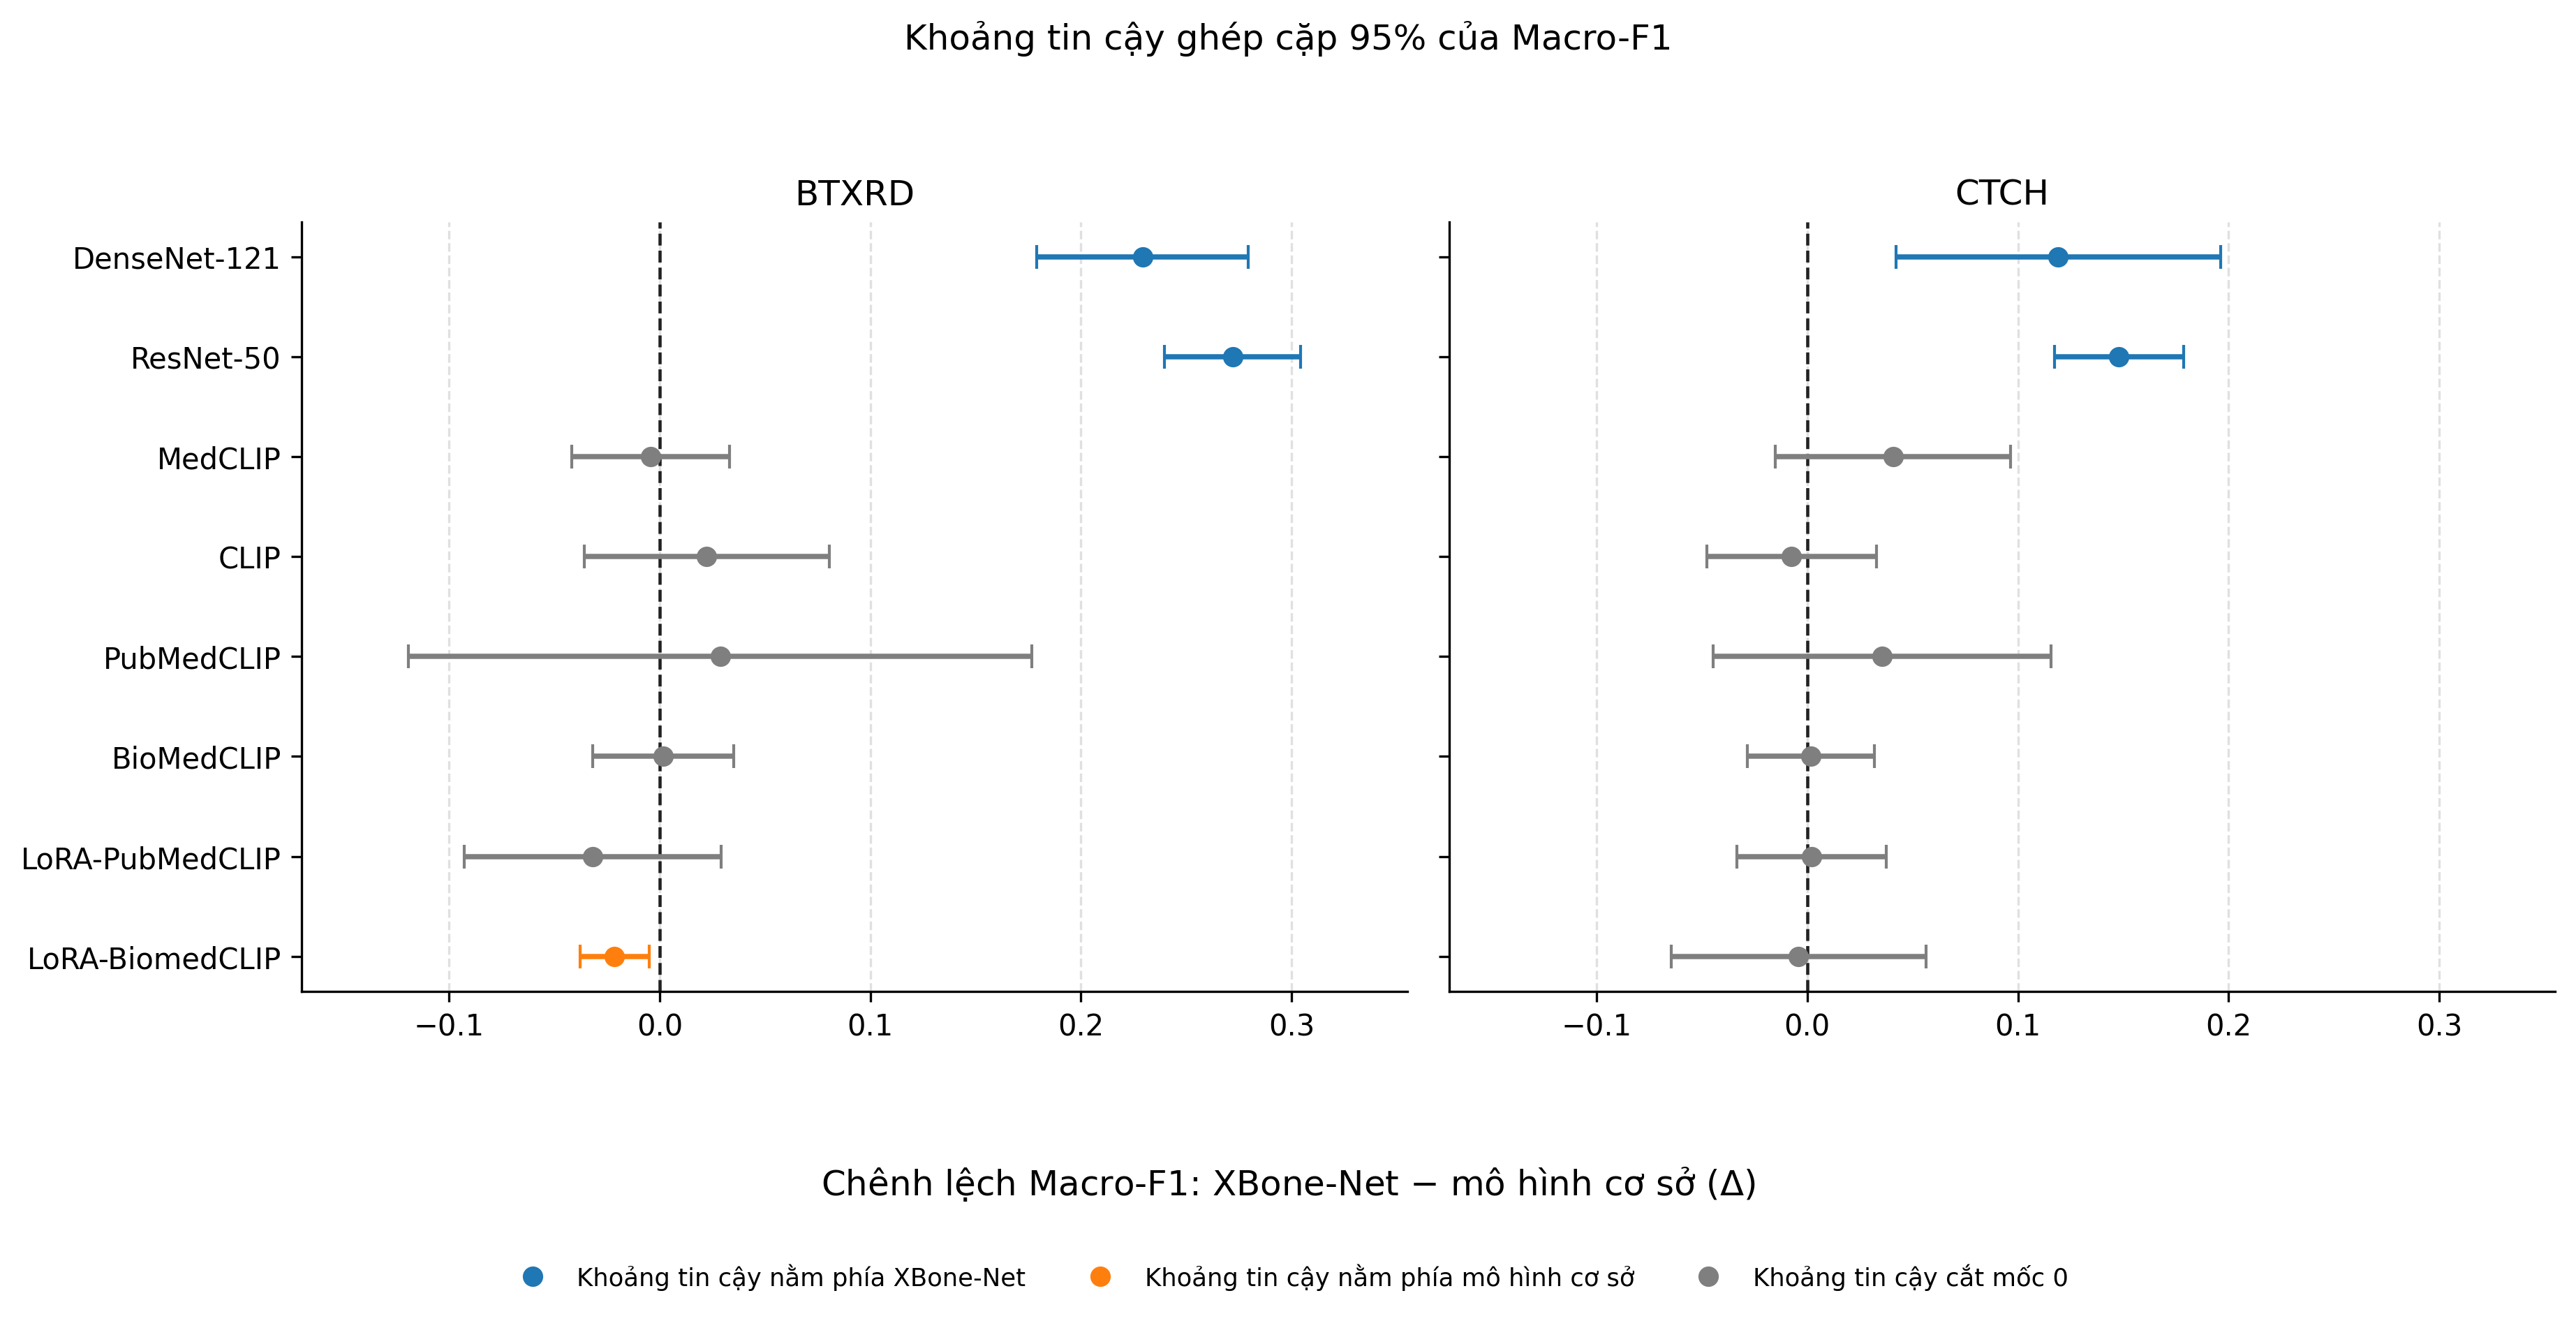
\includegraphics[width=1\linewidth]{generated/chapter4_results/full_shot_paired_f1_forest.png}
\caption{Khoảng ước lượng ghép cặp 95\% của chênh lệch điểm F1 trung bình theo lớp giữa XBone-Net và các mô hình cơ sở}
\label{fig:full_shot_paired_f1_forest}
\end{figure}

Khoảng ước lượng ghép cặp của chênh lệch điểm F1 trong Hình~\ref{fig:full_shot_paired_f1_forest} cho thấy XBone-Net cao hơn rõ rệt so với ResNet-50 và DenseNet-121 trên cả hai bộ dữ liệu, nhưng phần lớn khoảng so sánh với các mô hình thị giác--ngôn ngữ bao gồm mốc 0. Trên BTXRD, khoảng so sánh với LoRA-BiomedCLIP nghiêng về mô hình cơ sở. Do chỉ có ba cặp hạt giống, các khoảng này chủ yếu mô tả độ biến thiên của những lần huấn luyện hiện có và không được dùng để suy rộng thành phân phối hiệu năng rộng hơn.

Trên CTCH, ma trận nhầm lẫn tổng hợp ở Hình~\ref{fig:ctch_confusion_matrix} cho thấy độ nhạy cao ở các lớp gãy xương đùi, gãy xương gót, gãy cột sống thắt lưng, gãy xương ngón tay và gãy xương cổ chân. Các lớp có độ nhạy thấp gồm cắt cụt ngón tay, gãy cột sống ngực, gãy xương trụ và gãy xương thuyền. Cắt cụt ngón tay thường bị nhầm với gãy xương ngón tay, còn gãy cột sống ngực thường bị nhầm với gãy cột sống thắt lưng. Đây là các cặp có vị trí giải phẫu hoặc nội dung bệnh sử gần nhau. Lớp bình thường chỉ đạt độ nhạy trung bình $0{,}43$, cho thấy mô hình vẫn gán một phần đáng kể ảnh không tổn thương vào các lớp bệnh lý.

\begin{figure}[H]
\centering
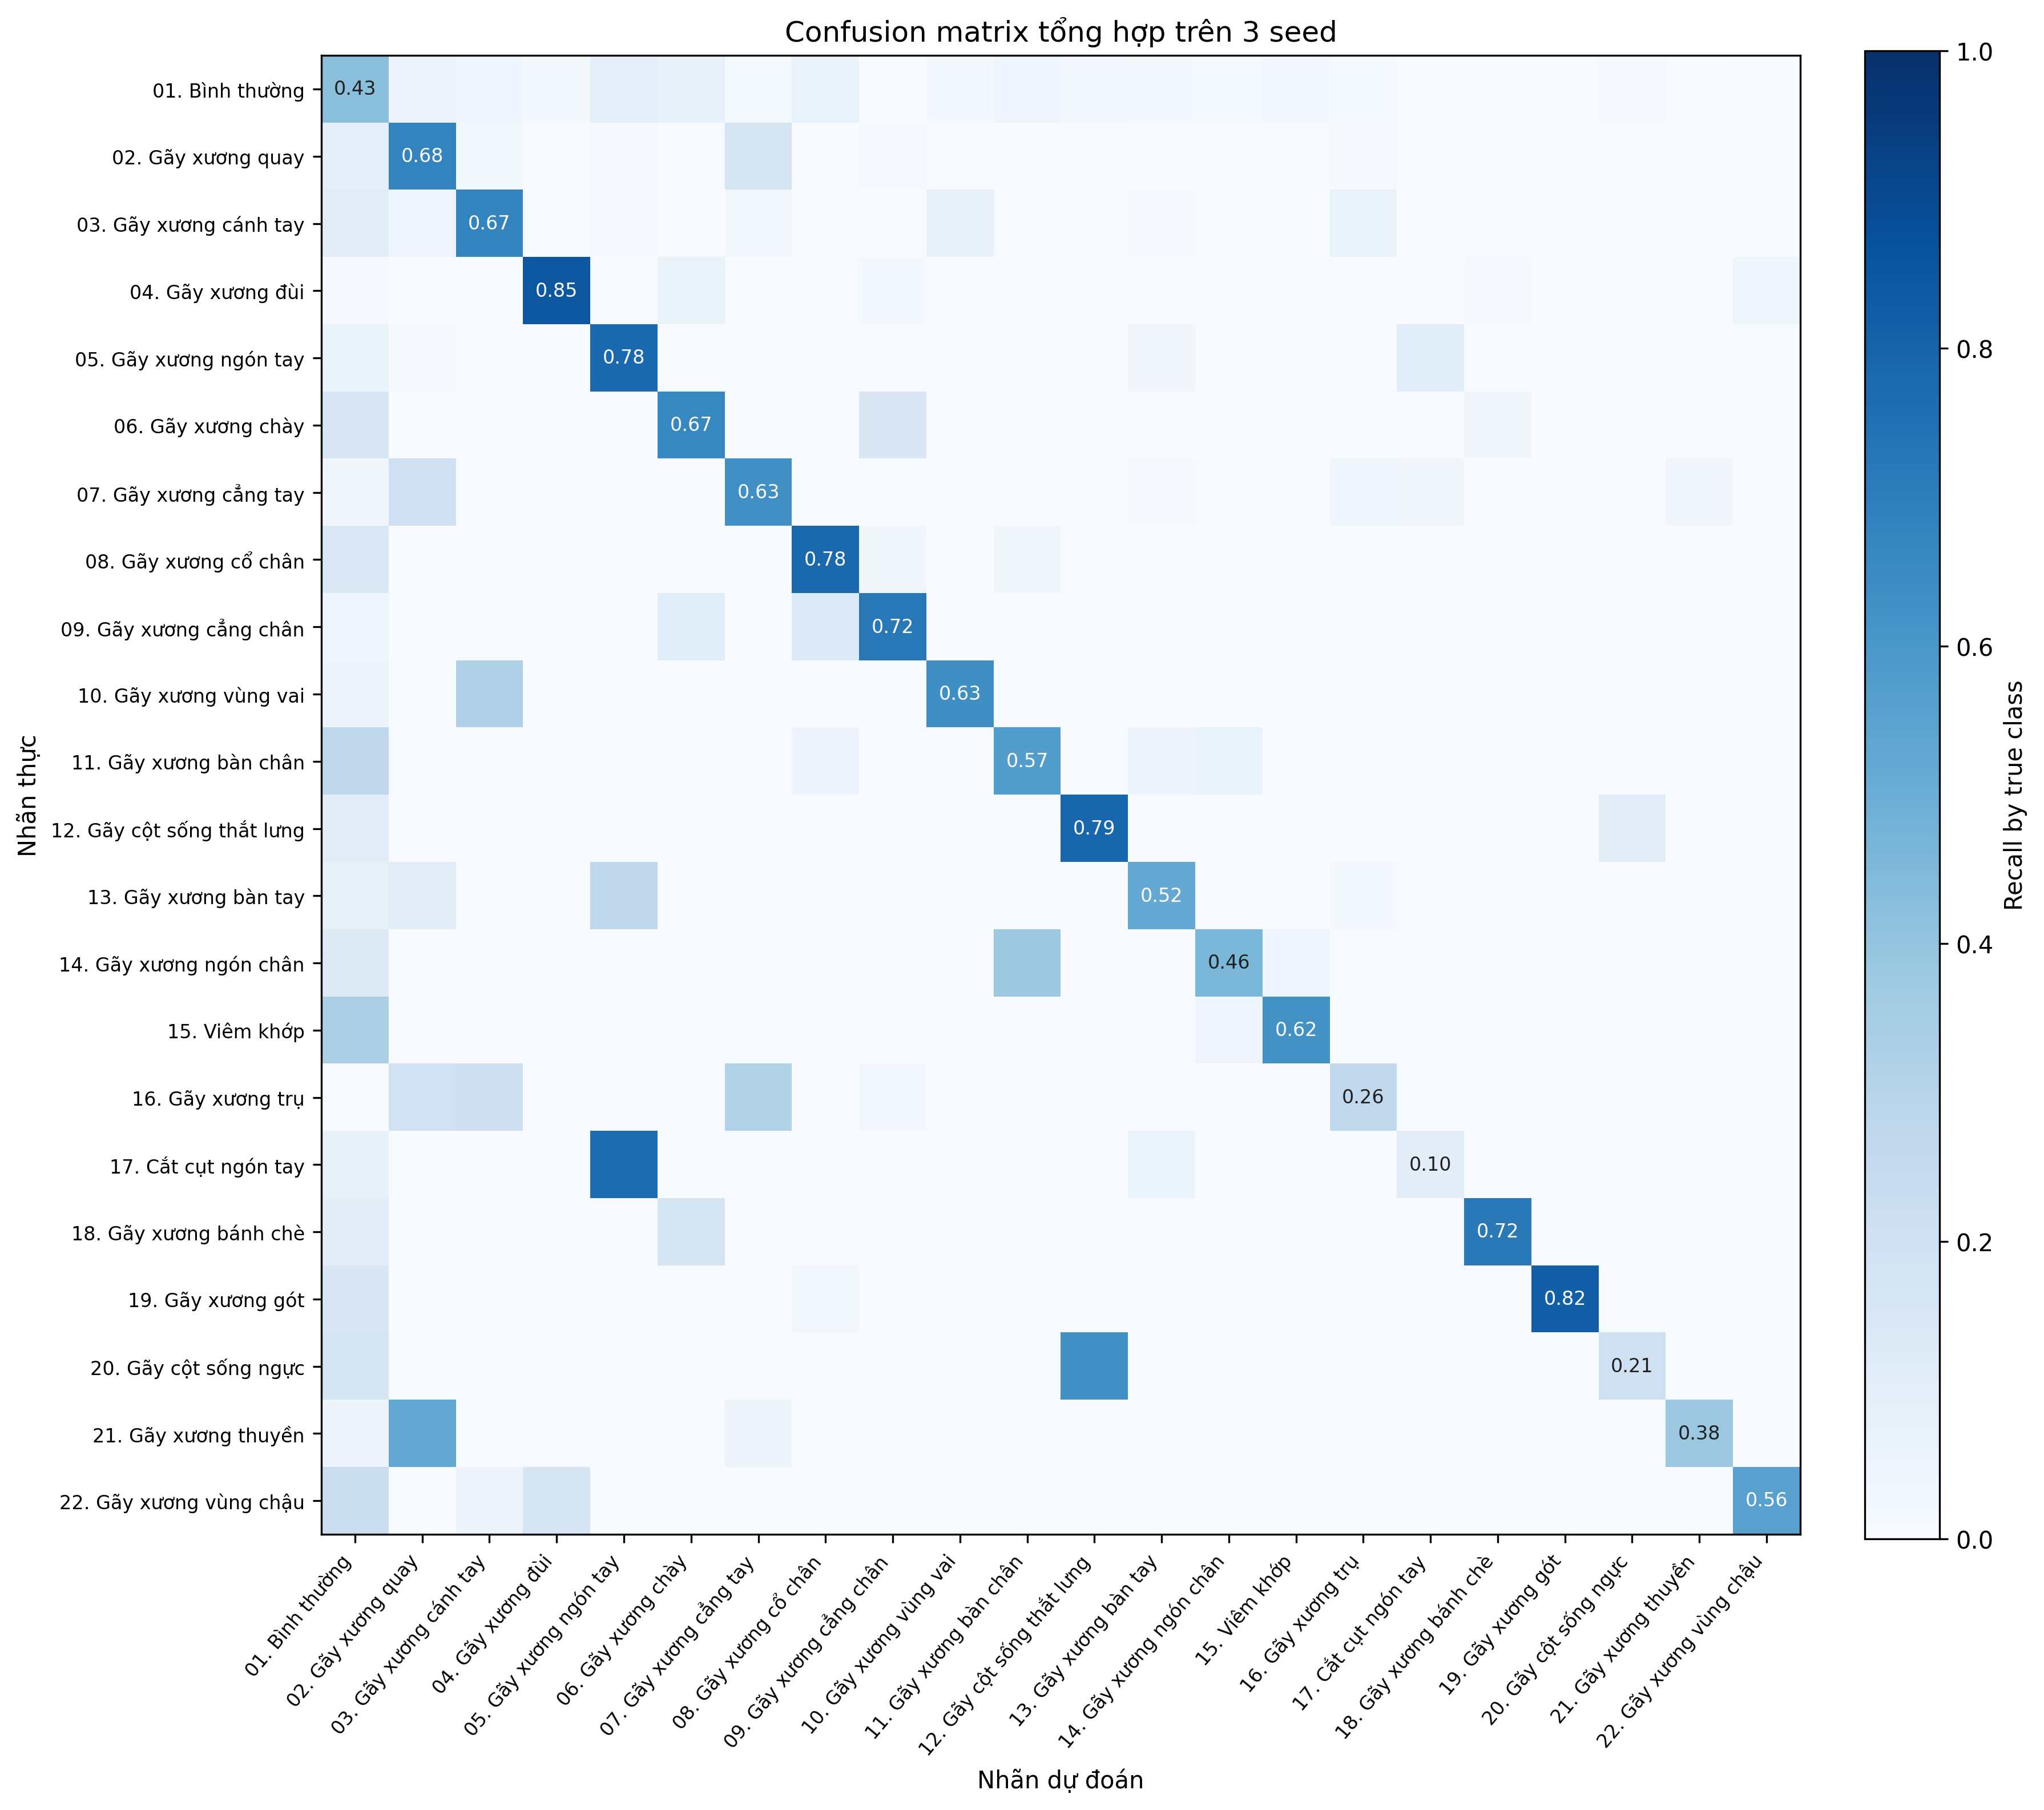
\includegraphics[width=0.92\linewidth]{generated/chapter4_results/ctch_xbone_net_confusion_matrix_3seed.png}
\caption{Ma trận nhầm lẫn chuẩn hóa theo nhãn thật của XBone-Net trên CTCH, tổng hợp trên ba hạt giống}
\label{fig:ctch_confusion_matrix}
\end{figure}

Hình~\ref{fig:ctch_pr_curve} và Hình~\ref{fig:ctch_roc_curve} làm rõ khoảng cách giữa chất lượng xếp hạng và quyết định lớp. Macro-AUROC đạt $0{,}947\pm0{,}025$, trong khi Macro-AUPRC đạt $0{,}619\pm0{,}014$. Đường cong độ chính xác dự đoán--độ nhạy vẫn cao hơn rõ rệt mức phổ biến trung bình $0{,}045$, nhưng độ chính xác dự đoán giảm nhanh khi độ nhạy tiến gần 1, phản ánh khó khăn trong việc duy trì độ chuẩn xác cao đồng thời trên các lớp hiếm.

\begin{figure}[H]
\centering
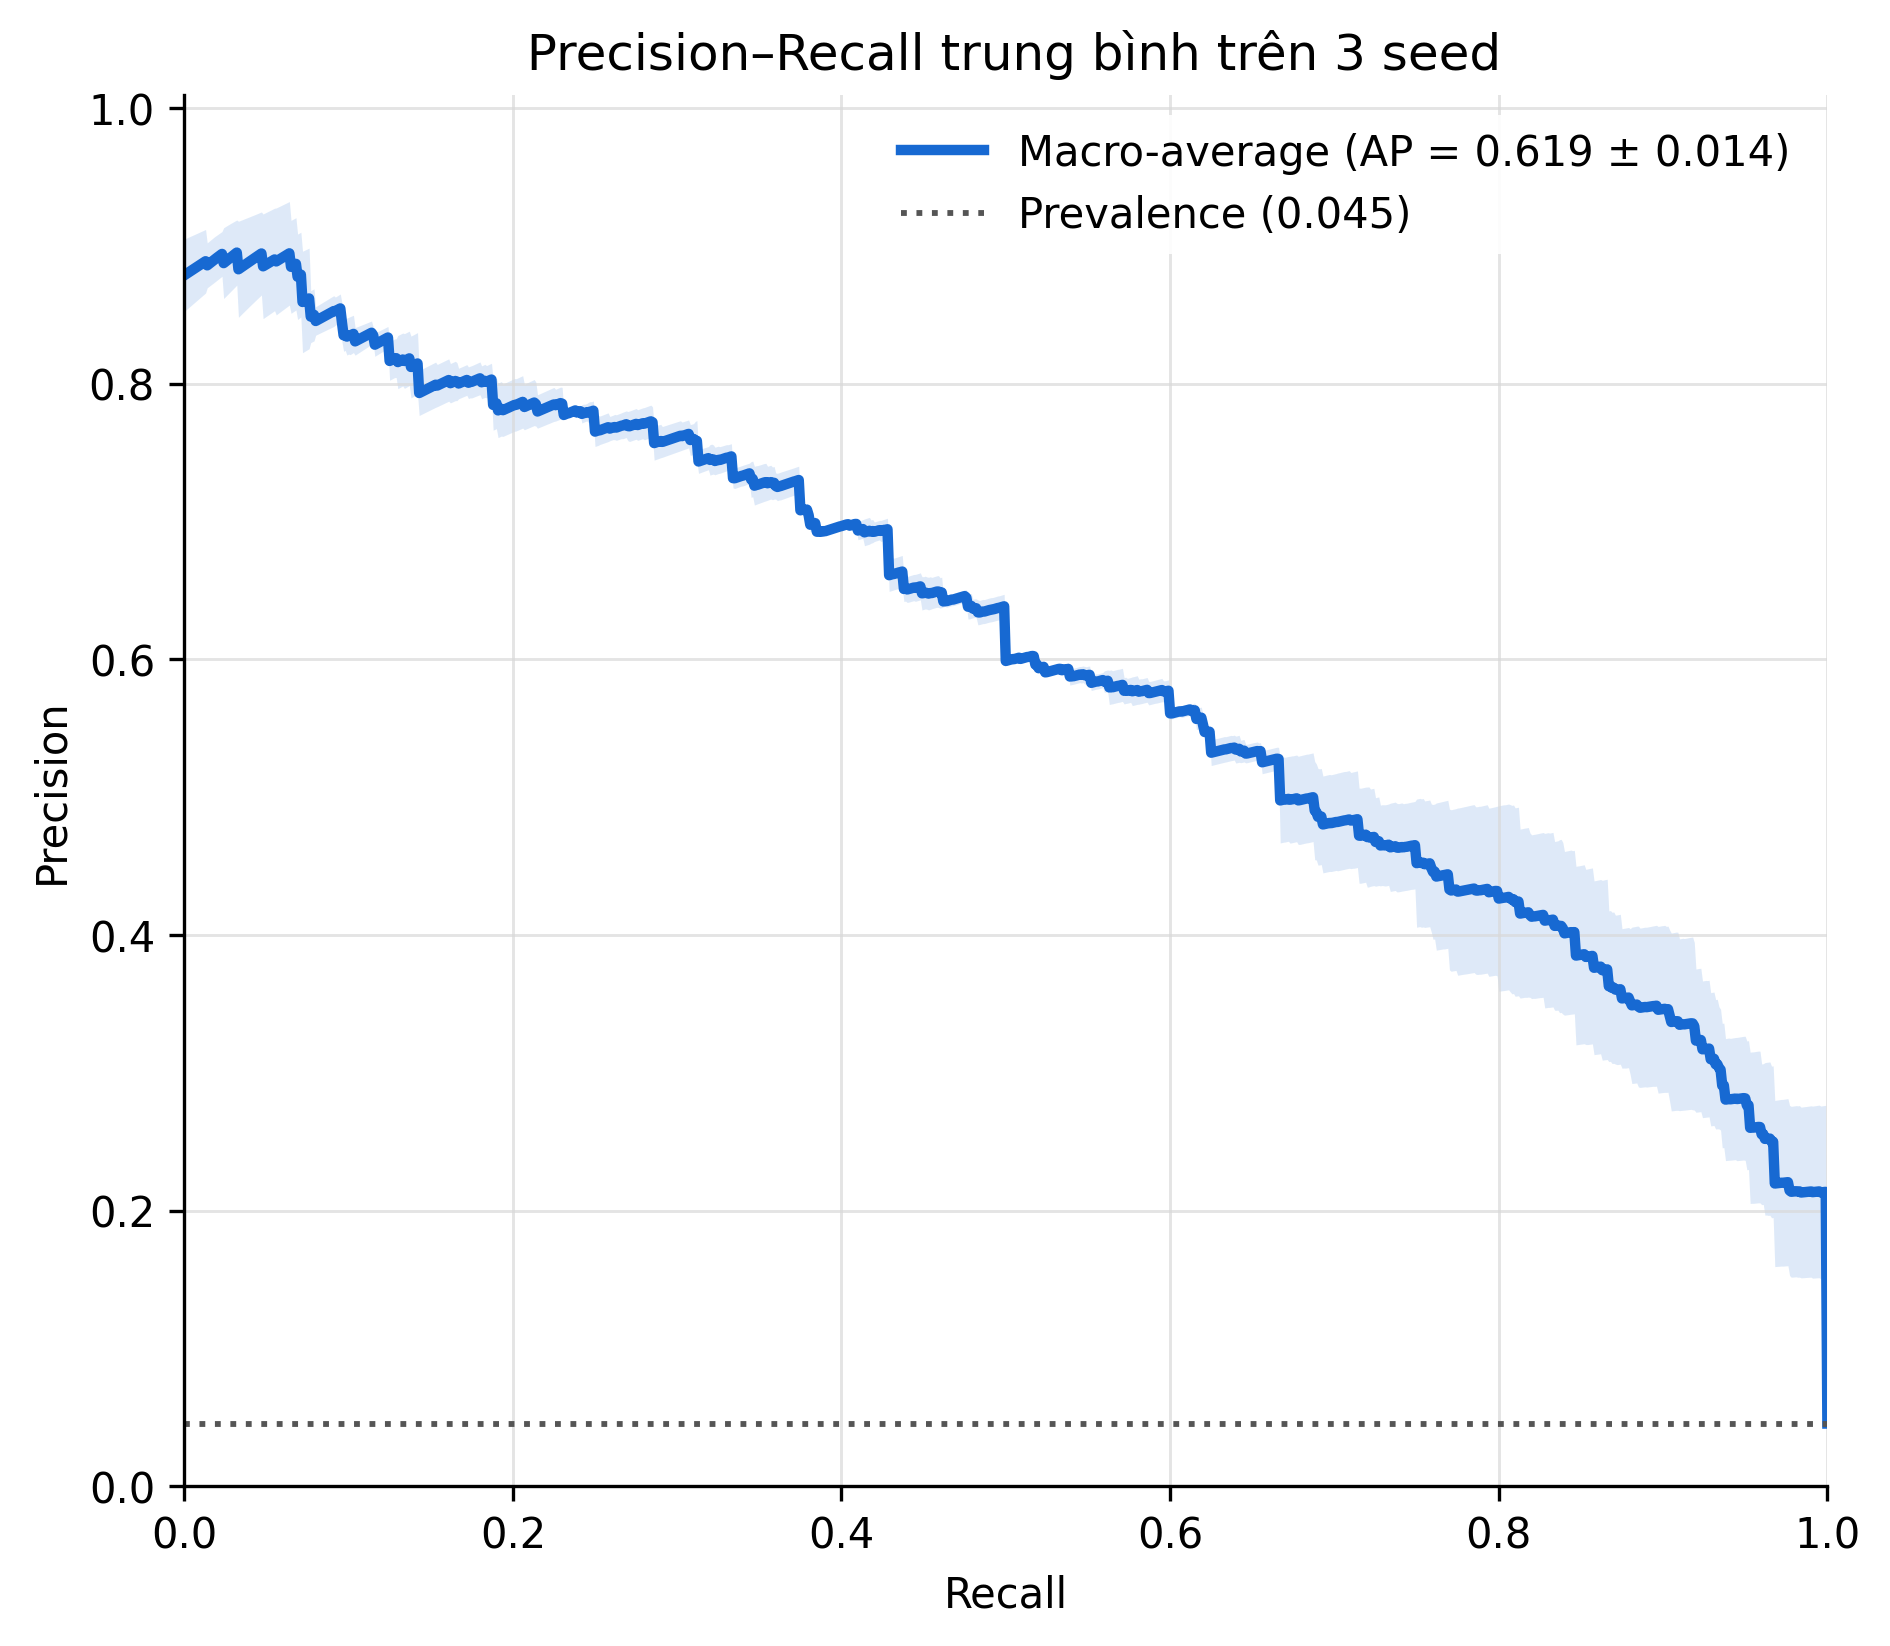
\includegraphics[width=0.57\linewidth]{generated/chapter4_results/ctch_xbone_net_pr_3seed.png}
\caption{Đường cong độ chính xác dự đoán--độ nhạy trung bình theo lớp của XBone-Net trên CTCH}
\label{fig:ctch_pr_curve}
\end{figure}

\begin{figure}[H]
\centering
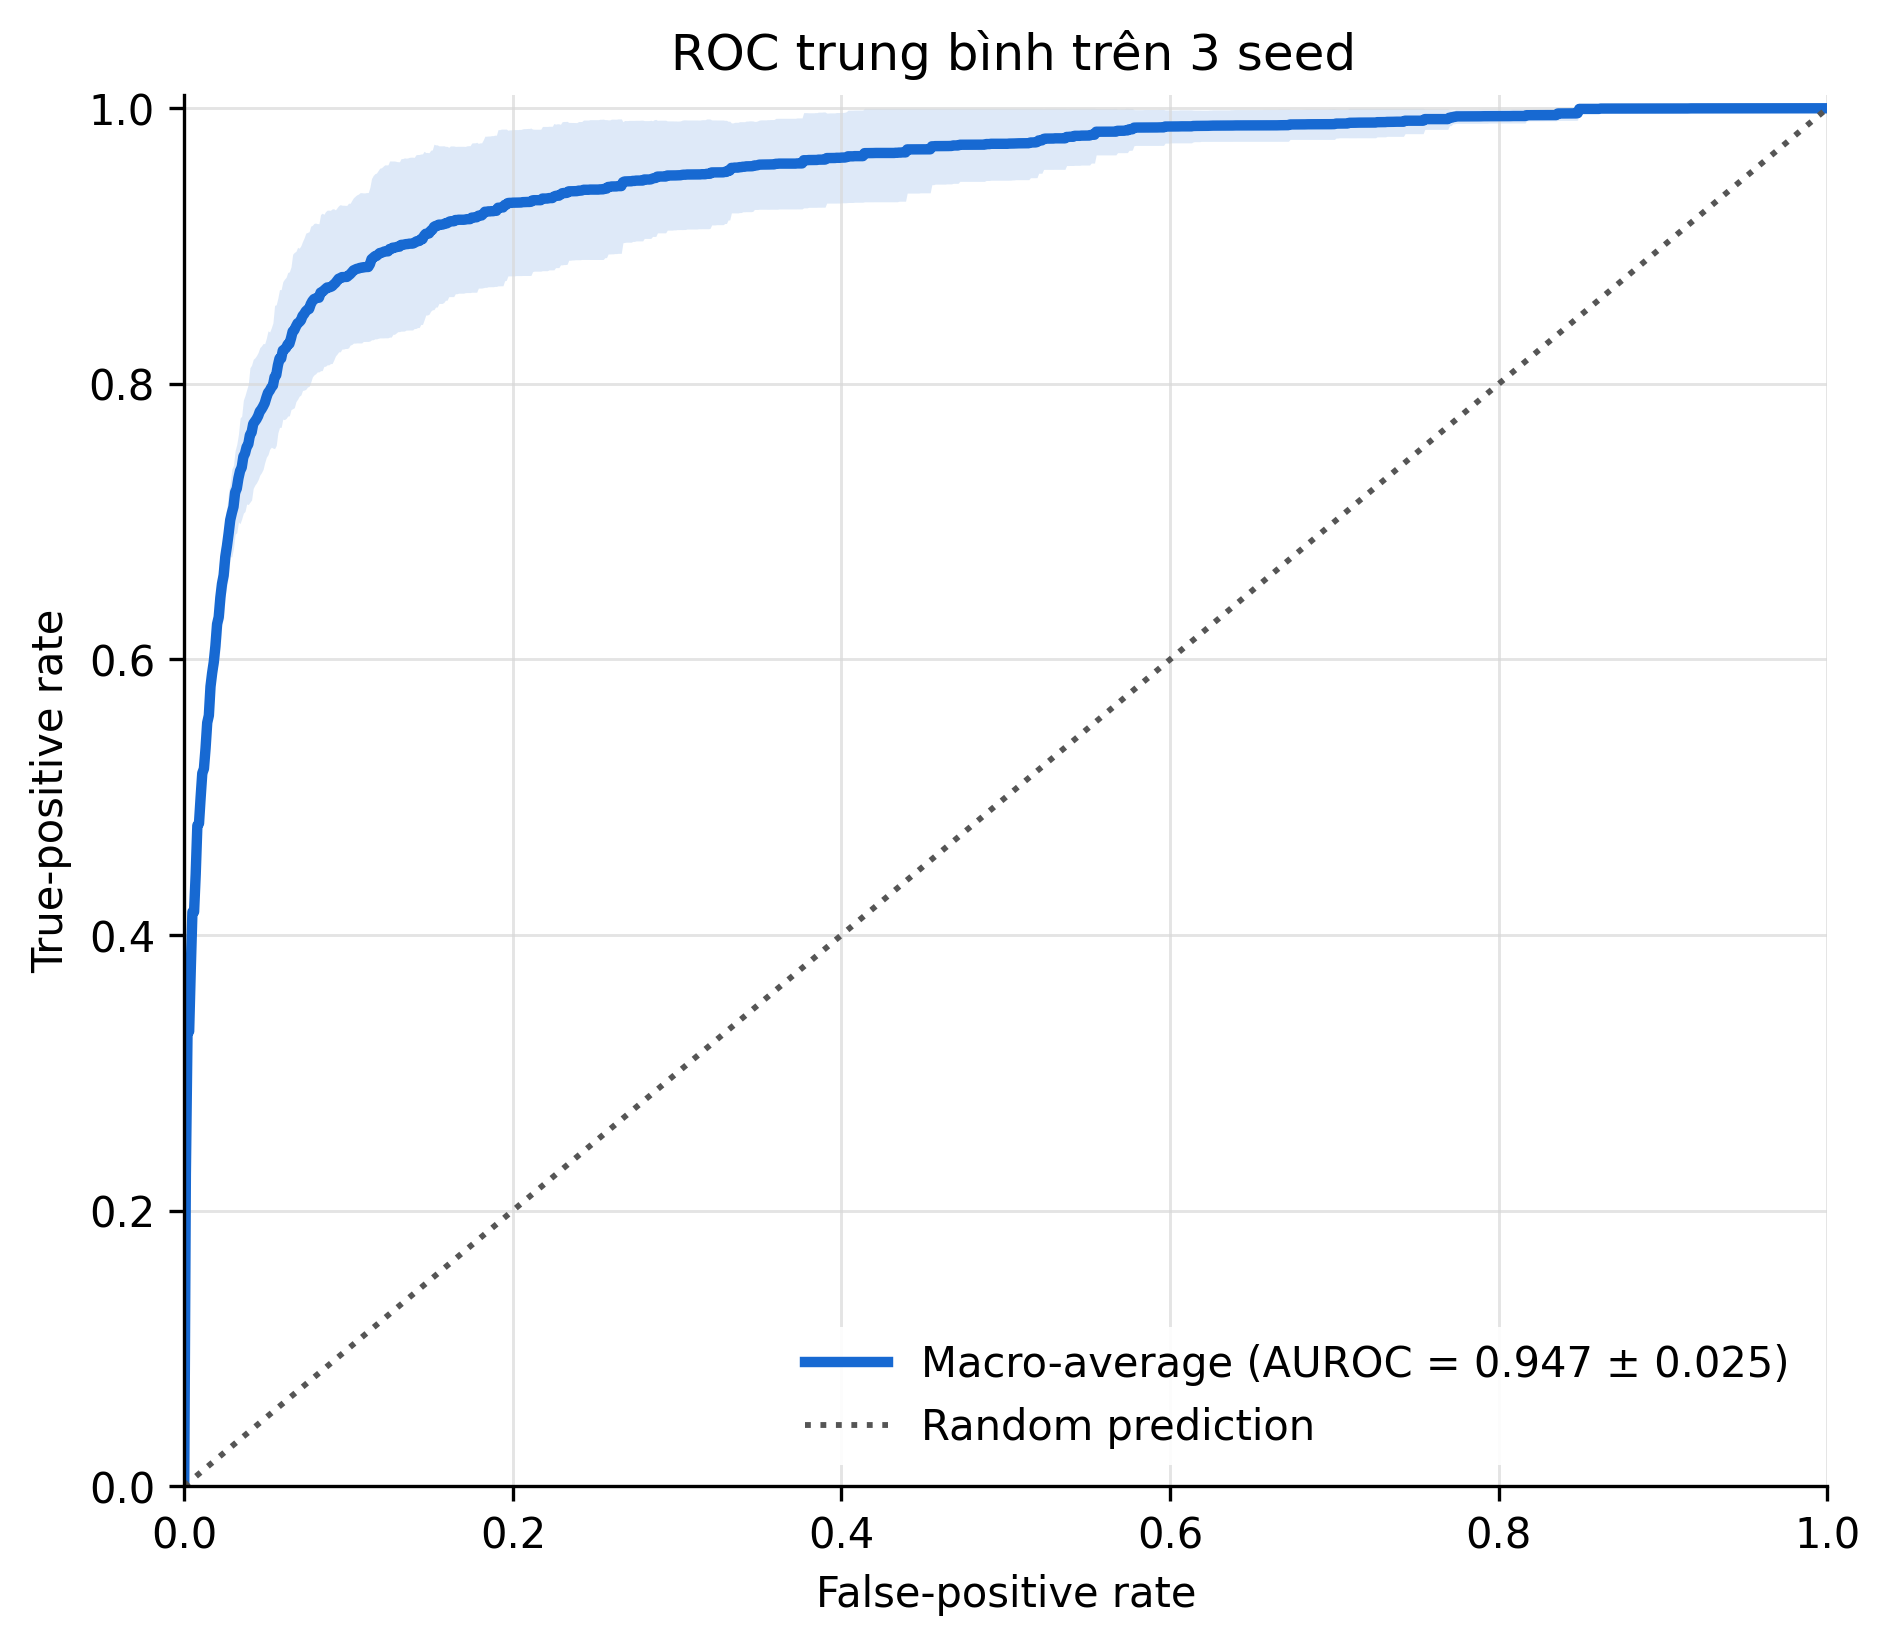
\includegraphics[width=0.57\linewidth]{generated/chapter4_results/ctch_xbone_net_roc_3seed.png}
\caption{Đường cong ROC trung bình theo lớp của XBone-Net trên CTCH}
\label{fig:ctch_roc_curve}
\end{figure}

Đường cong hiệu chỉnh trong Hình~\ref{fig:ctch_calibration} cho thấy sai số hiệu chỉnh kỳ vọng đạt $10{,}32\%\pm3{,}03\%$. Ở phần lớn các khoảng có độ tin cậy từ khoảng $0{,}6$ trở lên, độ chính xác quan sát thấp hơn độ tin cậy trung bình, cho thấy mô hình có xu hướng quá tự tin. Độ biến thiên giữa ba hạt giống tăng ở các khoảng tin cậy cao. Do đó, các xác suất Softmax hiện tại được xem là xác suất dự đoán chưa hiệu chỉnh và không nên được sử dụng độc lập như xác suất rủi ro lâm sàng.

\begin{figure}[H]
\centering
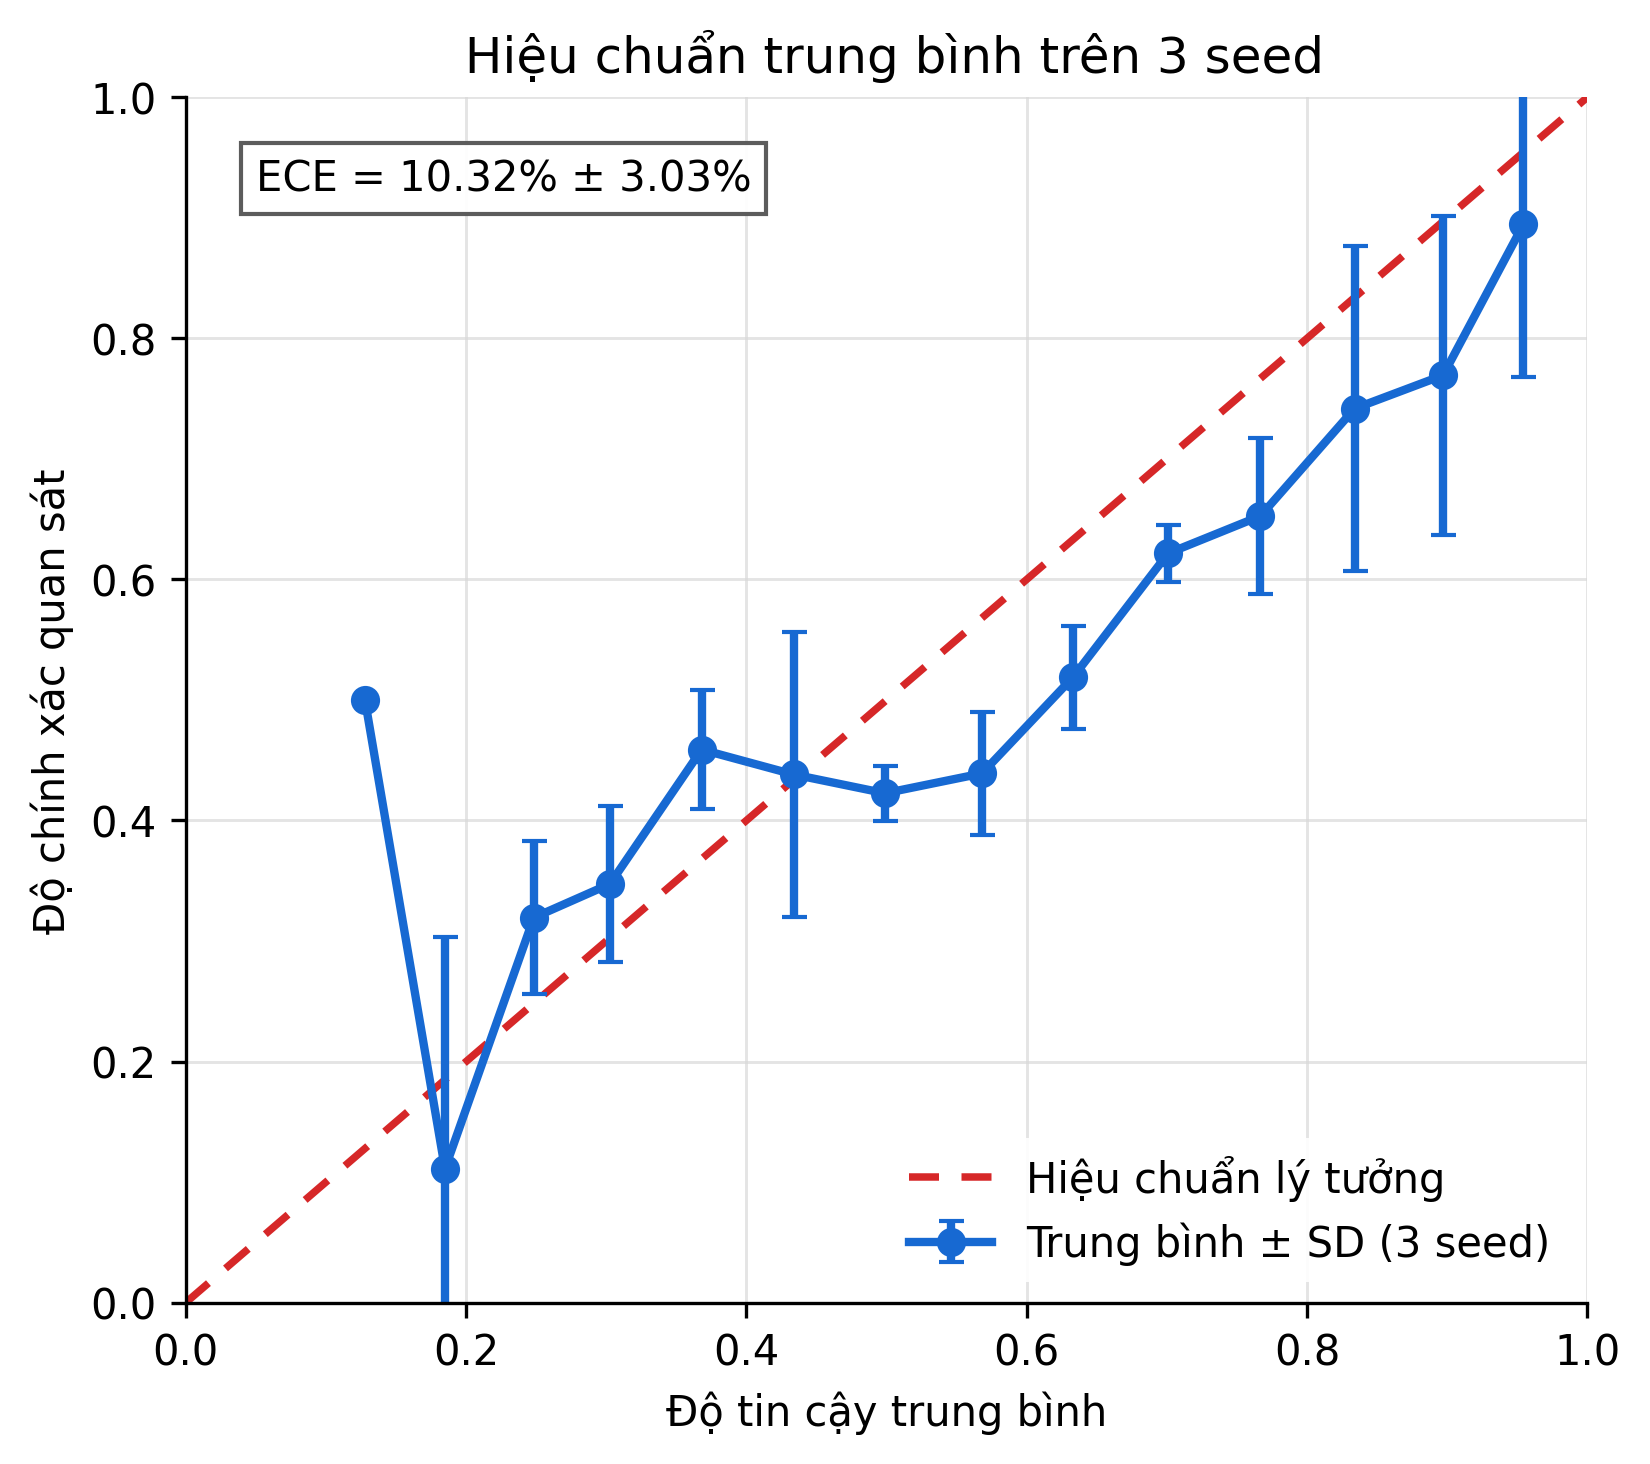
\includegraphics[width=0.78\linewidth]{generated/chapter4_results/ctch_xbone_net_calibration_3seed.png}
\caption{Đường cong hiệu chỉnh trung bình của XBone-Net trên CTCH qua ba hạt giống}
\label{fig:ctch_calibration}
\end{figure}

\subsection{Kết quả trong thiết lập ít mẫu}
\label{subsec:few_shot_results}
Bảng~\ref{tab:classification_few_shot} và Bảng~\ref{tab:classification_few_shot_ranking} cho thấy hiệu năng nhìn chung tăng theo ngân sách mẫu, nhưng thứ hạng giữa các mô hình thay đổi theo bộ dữ liệu và số mẫu mỗi lớp.

\begin{table}[H]
\centering
\small
\resizebox{\textwidth}{!}{%
\begin{tabular}{|l|l|l|c|c|c|}
\hline
\multicolumn{1}{|c|}{\textbf{Dữ liệu}} & \multicolumn{1}{c|}{\textbf{Thiết lập}} & \multicolumn{1}{c|}{\textbf{Mô hình}} & \multicolumn{1}{c|}{\textbf{Accuracy $\uparrow$}} & \multicolumn{1}{c|}{\textbf{Balanced Accuracy $\uparrow$}} & \multicolumn{1}{c|}{\textbf{Macro-F1 $\uparrow$}} \\ \hline
\multirow{9}{*}{BTXRD} & \multirow{3}{*}{1 mẫu} & LoRA-BiomedCLIP & $0.2782\pm0.0553$ & $0.2132\pm0.0468$ & $0.1699\pm0.0356$ \\ \cline{3-6}
 &  & LoRA-PubMedCLIP & $\mathbf{0.3164\pm0.1723}$ & $\mathbf{0.2507\pm0.0431}$ & $\mathbf{0.1818\pm0.0619}$ \\ \cline{3-6}
 &  & \cellcolor{gray!12}XBone-Net & \cellcolor{gray!12}$0.2480\pm0.0370$ & \cellcolor{gray!12}$0.2116\pm0.0503$ & \cellcolor{gray!12}$0.1620\pm0.0259$ \\ \cline{2-6}
 & \multirow{3}{*}{10 mẫu} & LoRA-BiomedCLIP & $0.6769\pm0.0381$ & $0.4671\pm0.0159$ & $0.4211\pm0.0123$ \\ \cline{3-6}
 &  & LoRA-PubMedCLIP & $0.6640\pm0.0615$ & $0.4441\pm0.0105$ & $0.4164\pm0.0157$ \\ \cline{3-6}
 &  & \cellcolor{gray!12}XBone-Net & \cellcolor{gray!12}$\mathbf{0.6889\pm0.0296}$ & \cellcolor{gray!12}$\mathbf{0.4771\pm0.0300}$ & \cellcolor{gray!12}$\mathbf{0.4302\pm0.0263}$ \\ \cline{2-6}
 & \multirow{3}{*}{20 mẫu} & LoRA-BiomedCLIP & $0.7311\pm0.0073$ & $0.5492\pm0.0244$ & $0.4876\pm0.0044$ \\ \cline{3-6}
 &  & LoRA-PubMedCLIP & $0.7369\pm0.0109$ & $0.5785\pm0.0158$ & $0.5132\pm0.0112$ \\ \cline{3-6}
 &  & \cellcolor{gray!12}XBone-Net & \cellcolor{gray!12}$\mathbf{0.7449\pm0.0166}$ & \cellcolor{gray!12}$\mathbf{0.5949\pm0.0258}$ & \cellcolor{gray!12}$\mathbf{0.5202\pm0.0300}$ \\ \hline
\multirow{9}{*}{CTCH} & \multirow{3}{*}{1 mẫu} & LoRA-BiomedCLIP & $0.2128\pm0.0116$ & $0.2830\pm0.0164$ & $0.2074\pm0.0034$ \\ \cline{3-6}
 &  & LoRA-PubMedCLIP & $0.1908\pm0.0496$ & $0.2850\pm0.0749$ & $0.1876\pm0.0434$ \\ \cline{3-6}
 &  & \cellcolor{gray!12}XBone-Net & \cellcolor{gray!12}$\mathbf{0.2342\pm0.0175}$ & \cellcolor{gray!12}$\mathbf{0.3351\pm0.0659}$ & \cellcolor{gray!12}$\mathbf{0.2236\pm0.0206}$ \\ \cline{2-6}
 & \multirow{3}{*}{10 mẫu} & LoRA-BiomedCLIP & $\mathbf{0.4036\pm0.0334}$ & $0.5558\pm0.0275$ & $0.4291\pm0.0165$ \\ \cline{3-6}
 &  & LoRA-PubMedCLIP & $0.3812\pm0.0158$ & $\mathbf{0.5629\pm0.0136}$ & $0.4186\pm0.0117$ \\ \cline{3-6}
 &  & \cellcolor{gray!12}XBone-Net & \cellcolor{gray!12}$0.3926\pm0.0511$ & \cellcolor{gray!12}$0.5590\pm0.0419$ & \cellcolor{gray!12}$\mathbf{0.4329\pm0.0357}$ \\ \cline{2-6}
 & \multirow{3}{*}{20 mẫu} & LoRA-BiomedCLIP & $0.4395\pm0.0269$ & $\mathbf{0.6136\pm0.0263}$ & $\mathbf{0.4803\pm0.0219}$ \\ \cline{3-6}
 &  & LoRA-PubMedCLIP & $\mathbf{0.4509\pm0.0195}$ & $0.5878\pm0.0230$ & $0.4649\pm0.0236$ \\ \cline{3-6}
 &  & \cellcolor{gray!12}XBone-Net & \cellcolor{gray!12}$0.4360\pm0.0183$ & \cellcolor{gray!12}$0.5856\pm0.0173$ & \cellcolor{gray!12}$0.4684\pm0.0063$ \\ \hline
\end{tabular}
}
\caption{Kết quả phân loại trong các thiết lập mẫu học hạn chế}
\label{tab:classification_few_shot}
\end{table}


\begin{table}[H]
\centering
\small
\begin{tabular}{|l|l|l|c|c|}
\hline
\multicolumn{1}{|c|}{\textbf{Dữ liệu}} & \multicolumn{1}{c|}{\textbf{Thiết lập}} & \multicolumn{1}{c|}{\textbf{Mô hình}} & \multicolumn{1}{c|}{\textbf{Macro-AUROC $\uparrow$}} & \multicolumn{1}{c|}{\textbf{Macro-AUPRC $\uparrow$}} \\ \hline
\multirow{9}{*}{BTXRD} & \multirow{3}{*}{1-shot} & LoRA-BiomedCLIP & $0.6319\pm0.0404$ & $0.2085\pm0.0342$ \\ \cline{3-5}
 &  & LoRA-PubMedCLIP & $\mathbf{0.6511\pm0.0259}$ & $\mathbf{0.2501\pm0.0364}$ \\ \cline{3-5}
 &  & \cellcolor{gray!12}XBone-Net & \cellcolor{gray!12}$0.6274\pm0.0274$ & \cellcolor{gray!12}$0.2035\pm0.0383$ \\ \cline{2-5}
 & \multirow{3}{*}{10-shot} & LoRA-BiomedCLIP & $\mathbf{0.8598\pm0.0144}$ & $0.4467\pm0.0173$ \\ \cline{3-5}
 &  & LoRA-PubMedCLIP & $0.8529\pm0.0190$ & $\mathbf{0.4606\pm0.0183}$ \\ \cline{3-5}
 &  & \cellcolor{gray!12}XBone-Net & \cellcolor{gray!12}$0.8577\pm0.0050$ & \cellcolor{gray!12}$0.4552\pm0.0330$ \\ \cline{2-5}
 & \multirow{3}{*}{20-shot} & LoRA-BiomedCLIP & $\mathbf{0.9271\pm0.0092}$ & $0.5420\pm0.0061$ \\ \cline{3-5}
 &  & LoRA-PubMedCLIP & $0.9205\pm0.0132$ & $0.5561\pm0.0067$ \\ \cline{3-5}
 &  & \cellcolor{gray!12}XBone-Net & \cellcolor{gray!12}$0.9163\pm0.0160$ & \cellcolor{gray!12}$\mathbf{0.5635\pm0.0395}$ \\ \hline
\multirow{9}{*}{CTCH} & \multirow{3}{*}{1-shot} & LoRA-BiomedCLIP & $0.8231\pm0.0212$ & $0.2357\pm0.0130$ \\ \cline{3-5}
 &  & LoRA-PubMedCLIP & $0.7904\pm0.0188$ & $0.2040\pm0.0257$ \\ \cline{3-5}
 &  & \cellcolor{gray!12}XBone-Net & \cellcolor{gray!12}$\mathbf{0.8645\pm0.0082}$ & \cellcolor{gray!12}$\mathbf{0.2882\pm0.0140}$ \\ \cline{2-5}
 & \multirow{3}{*}{10-shot} & LoRA-BiomedCLIP & $0.9353\pm0.0070$ & $0.4647\pm0.0268$ \\ \cline{3-5}
 &  & LoRA-PubMedCLIP & $\mathbf{0.9393\pm0.0065}$ & $\mathbf{0.4785\pm0.0053}$ \\ \cline{3-5}
 &  & \cellcolor{gray!12}XBone-Net & \cellcolor{gray!12}$0.9368\pm0.0108$ & \cellcolor{gray!12}$0.4540\pm0.0235$ \\ \cline{2-5}
 & \multirow{3}{*}{20-shot} & LoRA-BiomedCLIP & $0.9416\pm0.0143$ & $0.5088\pm0.0308$ \\ \cline{3-5}
 &  & LoRA-PubMedCLIP & $\mathbf{0.9501\pm0.0011}$ & $\mathbf{0.5263\pm0.0191}$ \\ \cline{3-5}
 &  & \cellcolor{gray!12}XBone-Net & \cellcolor{gray!12}$0.9457\pm0.0072$ & \cellcolor{gray!12}$0.5217\pm0.0147$ \\ \hline
\end{tabular}
\caption{Các độ đo xếp hạng xác suất trong các thiết lập mẫu hạn chế}
\label{tab:classification_few_shot_ranking}
\end{table}


Trên BTXRD, XBone-Net đạt điểm F1 $0{,}1620\pm0{,}0259$ ở mức một mẫu và thấp hơn hai mô hình cơ sở. Tại mức 10 và 20 mẫu, XBone-Net dẫn đầu với các giá trị lần lượt $0{,}4302\pm0{,}0263$ và $0{,}5202\pm0{,}0300$. Trên CTCH, XBone-Net dẫn đầu ở mức một mẫu với $0{,}2236\pm0{,}0206$ và ở mức 10 mẫu với $0{,}4329\pm0{,}0357$, nhưng thấp hơn LoRA-BiomedCLIP tại mức 20 mẫu.

Khi tăng từ một lên 10 mẫu, điểm F1 của XBone-Net tăng $0{,}2682$ điểm trên BTXRD và $0{,}2093$ điểm trên CTCH. Mức tăng từ 10 lên 20 mẫu giảm còn $0{,}0900$ và $0{,}0355$ điểm. Xu hướng này gợi ý lợi ích biên giảm khi bổ sung mẫu, nhưng ba mức ngân sách chưa đủ để mô tả đầy đủ đường học. Độ lệch chuẩn tương đối lớn ở một số thiết lập, đặc biệt tại 10 và 20 mẫu trên BTXRD và 10 mẫu trên CTCH, cho thấy kết quả còn nhạy với tập mẫu được chọn theo từng hạt giống.

\subsection{Hiệu quả tham số và chi phí suy luận}
\label{subsec:rq3_adaptation_results}
Bảng~\ref{tab:rq3_adaptation} đối chiếu ba mức thích nghi bộ mã hóa nền tảng trên CTCH. XBone-Net sử dụng thích nghi hạng thấp và cập nhật $8{,}63$ triệu tham số, tương đương $4{,}22\%$ tổng số tham số, trong khi tinh chỉnh toàn bộ cập nhật $199{,}43$ triệu tham số. Cấu hình thích nghi hạng thấp đạt điểm F1 trung bình theo lớp $0{,}5558\pm0{,}0072$ và Macro-AUPRC $0{,}6189\pm0{,}0145$, cao hơn tinh chỉnh toàn bộ lần lượt $0{,}0146$ và $0{,}0357$ điểm. Macro-AUROC của hai cấu hình gần tương đương. Kết quả cho thấy việc giới hạn phạm vi cập nhật vẫn duy trì hiệu năng cạnh tranh trên dữ liệu hiện có.

\begin{table}[H]
\centering
\scriptsize
\setlength{\tabcolsep}{4pt}
\renewcommand{\arraystretch}{1.12}
\resizebox{\textwidth}{!}{%
\begin{tabular}{|l|c|c|c|c|c|}
\hline
\textbf{Mức thích nghi backbone} &
\textbf{Tham số cập nhật} &
\textbf{Macro-F1 $\uparrow$} &
\textbf{Macro-AUROC $\uparrow$} &
\textbf{Macro-AUPRC $\uparrow$} &
\textbf{Thời gian thực $\downarrow$} \\ \hline
Đóng băng backbone &
$3{.}49$M ($1{.}75\%$) &
$0{.}5405\pm0{.}0061$ &
$0{.}9502\pm0{.}0105$ &
$0{.}5641\pm0{.}0091$ &
Không lưu \\ \hline
\cellcolor{gray!12}LoRA (XBone-Net) &
\cellcolor{gray!12}$8{.}63$M ($4{.}22\%$) &
\cellcolor{gray!12}$\mathbf{0{.}5558\pm0{.}0072}$ &
\cellcolor{gray!12}$0{.}9473\pm0{.}0246$ &
\cellcolor{gray!12}$\mathbf{0{.}6189\pm0{.}0145}$ &
\cellcolor{gray!12}$2{.}61\pm0{.}44$ giờ ($n=3$) \\ \hline
Tinh chỉnh toàn bộ &
$199{.}43$M ($100\%$) &
$0{.}5412\pm0{.}0089$ &
$\mathbf{0{.}9507\pm0{.}0091}$ &
$0{.}5832\pm0{.}0192$ &
$1{.}94$ giờ ($n=1$) \\ \hline
\end{tabular}%
}
\caption{Đánh đổi mức thích nghi backbone trên CTCH phục vụ RQ3; thời gian là wall-clock và số lần đo được ghi riêng}
\label{tab:rq3_adaptation}
\end{table}


Số tham số của ba mô hình sử dụng thích nghi hạng thấp trong thiết lập toàn bộ dữ liệu được trình bày tại Bảng~\ref{tab:efficiency_full_shot_params}. XBone-Net có khoảng $204{,}54$ triệu tham số và cập nhật $8{,}63$ triệu tham số. Mức này cao hơn LoRA-BiomedCLIP và LoRA-PubMedCLIP vì XBone-Net bổ sung mô-đun tổng hợp ảnh cục bộ, cơ chế dung hợp và đầu phân lớp theo tâm lớp. Tuy vậy, tỷ lệ tham số được cập nhật vẫn chỉ bằng $4{,}22\%$, thấp hơn đáng kể so với tinh chỉnh toàn bộ. Số tham số gần như không thay đổi giữa BTXRD và CTCH, còn phần chênh lệch nhỏ đến từ số lớp đầu ra.

\begin{table}[htbp]
\centering
\resizebox{\columnwidth}{!}{%
\begin{tabular}{|c|l|c|c|c|}
\hline
\textbf{Dữ liệu} & \multicolumn{1}{c|}{\textbf{Mô hình}} & \textbf{Tổng tham số} & \textbf{Tham số huấn luyện} & \textbf{Tỷ lệ (\%)} \\ \hline
\multirow{3}{*}{BTXRD} & LoRA-BiomedCLIP              & 201,447,179                    & 5,544,458                    & 2.75\%                    \\ \cline{2-5} 
                       & LoRA-PubMedCLIP              & 155,052,299                    & 3,774,986                    & 2.43\%                    \\ \cline{2-5} 
                       & \cellcolor{gray!12}XBone-Net & \cellcolor{gray!12}204,535,308 & \cellcolor{gray!12}8,632,587 & \cellcolor{gray!12}4.22\% \\ \hline
\multirow{3}{*}{CTCH}  & LoRA-BiomedCLIP              & 201,453,335                    & 5,550,614                    & 2.76\%                    \\ \cline{2-5} 
                       & LoRA-PubMedCLIP              & 155,058,455                    & 3,781,142                    & 2.44\%                    \\ \cline{2-5} 
                       & \cellcolor{gray!12}XBone-Net & \cellcolor{gray!12}204,535,320 & \cellcolor{gray!12}8,632,599 & \cellcolor{gray!12}4.22\% \\ \hline
\end{tabular}%
}
\caption{Đánh giá số lượng tham số của các mô hình khi sử dụng toàn bộ dữ liệu}
\label{tab:efficiency_full_shot_params}
\end{table}

\begin{table}[htbp]
\centering
\resizebox{\columnwidth}{!}{%
\begin{tabular}{|c|l|c|c|c|c|}
\hline
\textbf{Dữ liệu} &
  \multicolumn{1}{c|}{\textbf{Mô hình}} &
  \textbf{GFLOPs} &
  \textbf{Thông lượng} &
  \textbf{\begin{tabular}[c]{@{}c@{}}Độ trễ \\ trung bình\end{tabular}} &
  \textbf{\begin{tabular}[c]{@{}c@{}}Bộ nhớ GPU \\ cực đại\end{tabular}} \\ \hline
\multirow{3}{*}{BTXRD} & LoRA-BiomedCLIP              & 83.321                     & 30.6                    & 36.25                    & 792.6                    \\ \cline{2-6} 
                       & LoRA-PubMedCLIP              & 15.198                     & 33.3                    & 43.87                    & 603.6                    \\ \cline{2-6} 
                       & \cellcolor{gray!12}XBone-Net & \cellcolor{gray!12}229.020 & \cellcolor{gray!12}17.7 & \cellcolor{gray!12}64.92 & \cellcolor{gray!12}835.5 \\ \hline
\multirow{3}{*}{CTCH}  & LoRA-BiomedCLIP              & 83.321                     & 38.3                    & 30.16                    & 792.6                    \\ \cline{2-6} 
                       & LoRA-PubMedCLIP              & 15.198                     & 37.7                    & 34.56                    & 603.6                    \\ \cline{2-6} 
                       & \cellcolor{gray!12}XBone-Net & \cellcolor{gray!12}229.020 & \cellcolor{gray!12}13.4 & \cellcolor{gray!12}87.15 & \cellcolor{gray!12}835.6 \\ \hline
\end{tabular}%
}
\caption{Đánh giá chi phí tính toán và tốc độ suy luận của các mô hình khi sử dụng toàn bộ dữ liệu}
\label{tab:efficiency_full_shot_compute}
\end{table}

Bảng~\ref{tab:efficiency_full_shot_compute} cho thấy hiệu quả tham số khi huấn luyện không đồng nghĩa với chi phí suy luận thấp. XBone-Net cần $229{,}020$ GFLOPs trên mỗi mẫu, cao gấp khoảng $2{,}75$ lần LoRA-BiomedCLIP và $15{,}07$ lần LoRA-PubMedCLIP. Nguyên nhân chính là mỗi mẫu được mã hóa bằng một ảnh toàn cục cùng bốn vùng ảnh cục bộ trước khi các biểu diễn được tổng hợp và dung hợp với văn bản.

Trên BTXRD, XBone-Net đạt thông lượng $17{,}7$ mẫu mỗi giây và độ trễ trung bình $64{,}92$ mili giây mỗi mẫu, trong khi hai mô hình cơ sở đạt từ $30{,}6$ đến $33{,}3$ mẫu mỗi giây. Trên CTCH, thông lượng của XBone-Net giảm còn $13{,}4$ mẫu mỗi giây và độ trễ tăng lên $87{,}15$ mili giây mỗi mẫu, so với thông lượng từ $37{,}7$ đến $38{,}3$ mẫu mỗi giây của hai mô hình cơ sở. Bộ nhớ đồ họa cực đại của XBone-Net đạt khoảng $835{,}5$ MiB, cao hơn LoRA-BiomedCLIP khoảng $5\%$ và LoRA-PubMedCLIP khoảng $38\%$. Vì phép đo chỉ bao gồm lan truyền tiến sau khi dữ liệu đã được đưa lên bộ nhớ đồ họa, các giá trị này phản ánh chi phí của kiến trúc mô hình hơn là thời gian đọc dữ liệu và tiền xử lý.

\begin{table}[H]
\centering
\scriptsize
\setlength{\tabcolsep}{3pt}
\resizebox{\textwidth}{!}{%
\begin{tabular}{|>{\centering\arraybackslash}m{1.5cm}|>{\centering\arraybackslash}m{1.8cm}|>{\raggedright\arraybackslash}m{3.5cm}|c|c|c|}
\hline
\multicolumn{1}{|c|}{\textbf{Dữ liệu}} & \multicolumn{1}{c|}{\textbf{Kịch bản}} & \multicolumn{1}{c|}{\textbf{Mô hình}} & \multicolumn{1}{c|}{\textbf{Tổng tham số}} & \multicolumn{1}{c|}{\textbf{Tham số huấn luyện}} & \multicolumn{1}{c|}{\textbf{Tỷ lệ (\%)}} \\ \hline
\multirow[c]{9}{=}{\centering BTXRD} & \multirow[c]{3}{=}{\centering 1 mẫu} & LoRA-BiomedCLIP & 201,447,179 & 5,544,458 & 2.75\% \\ \cline{3-6}
 &  & LoRA-PubMedCLIP & 155,052,299 & 3,774,986 & 2.43\% \\ \cline{3-6}
 &  & \cellcolor{gray!12}XBone-Net & \cellcolor{gray!12}204,535,308 & \cellcolor{gray!12}8,632,587 & \cellcolor{gray!12}4.22\% \\ \cline{2-6}
 & \multirow[c]{3}{=}{\centering 10 mẫu} & LoRA-BiomedCLIP & 201,447,179 & 5,544,458 & 2.75\% \\ \cline{3-6}
 &  & LoRA-PubMedCLIP & 155,052,299 & 3,774,986 & 2.43\% \\ \cline{3-6}
 &  & \cellcolor{gray!12}XBone-Net & \cellcolor{gray!12}204,535,308 & \cellcolor{gray!12}8,632,587 & \cellcolor{gray!12}4.22\% \\ \cline{2-6}
 & \multirow[c]{3}{=}{\centering 20 mẫu} & LoRA-BiomedCLIP & 201,447,179 & 5,544,458 & 2.75\% \\ \cline{3-6}
 &  & LoRA-PubMedCLIP & 155,052,299 & 3,774,986 & 2.43\% \\ \cline{3-6}
 &  & \cellcolor{gray!12}XBone-Net & \cellcolor{gray!12}204,535,308 & \cellcolor{gray!12}8,632,587 & \cellcolor{gray!12}4.22\% \\ \hline
\multirow[c]{9}{=}{\centering CTCH} & \multirow[c]{3}{=}{\centering 1 mẫu} & LoRA-BiomedCLIP & 201,453,335 & 5,550,614 & 2.76\% \\ \cline{3-6}
 &  & LoRA-PubMedCLIP & 155,058,455 & 3,781,142 & 2.44\% \\ \cline{3-6}
 &  & \cellcolor{gray!12}XBone-Net & \cellcolor{gray!12}204,535,320 & \cellcolor{gray!12}8,632,599 & \cellcolor{gray!12}4.22\% \\ \cline{2-6}
 & \multirow[c]{3}{=}{\centering 10 mẫu} & LoRA-BiomedCLIP & 201,453,335 & 5,550,614 & 2.76\% \\ \cline{3-6}
 &  & LoRA-PubMedCLIP & 155,058,455 & 3,781,142 & 2.44\% \\ \cline{3-6}
 &  & \cellcolor{gray!12}XBone-Net & \cellcolor{gray!12}204,535,320 & \cellcolor{gray!12}8,632,599 & \cellcolor{gray!12}4.22\% \\ \cline{2-6}
 & \multirow[c]{3}{=}{\centering 20 mẫu} & LoRA-BiomedCLIP & 201,453,335 & 5,550,614 & 2.76\% \\ \cline{3-6}
 &  & LoRA-PubMedCLIP & 155,058,455 & 3,781,142 & 2.44\% \\ \cline{3-6}
 &  & \cellcolor{gray!12}XBone-Net & \cellcolor{gray!12}204,535,320 & \cellcolor{gray!12}8,632,599 & \cellcolor{gray!12}4.22\% \\ \hline
\end{tabular}%
}
\caption{Đánh giá số lượng tham số của các mô hình trong thiết lập mẫu học hạn chế}
\label{tab:efficiency_few_shot_params}
\end{table}

\begin{table}[H]
\centering
\scriptsize
\setlength{\tabcolsep}{3pt}
\resizebox{\textwidth}{!}{%
\begin{tabular}{|>{\centering\arraybackslash}m{1.5cm}|>{\centering\arraybackslash}m{1.8cm}|>{\raggedright\arraybackslash}m{3.5cm}|c|c|c|c|}
\hline
\multirow[c]{2}{=}{\centering\textbf{Dữ liệu}} & \multirow[c]{2}{=}{\centering\textbf{Kịch bản}} & \multirow[c]{2}{=}{\centering\textbf{Mô hình}} & \multicolumn{1}{c|}{\textbf{GFLOPs}} & \multicolumn{1}{c|}{\textbf{Thông lượng}} & \multicolumn{1}{c|}{\textbf{Độ trễ trung bình}} & \multicolumn{1}{c|}{\textbf{Peak GPU}} \\
 & & & \multicolumn{1}{c|}{\textbf{(GFLOP/mẫu)}} & \multicolumn{1}{c|}{\textbf{(mẫu/s)}} & \multicolumn{1}{c|}{\textbf{(ms/mẫu)}} & \multicolumn{1}{c|}{\textbf{(MiB)}} \\ \hline
\multirow[c]{9}{=}{\centering BTXRD} & \multirow[c]{3}{=}{\centering 1 mẫu} & LoRA-BiomedCLIP & 83.321 & 28.8 & 37.32 & 792.6 \\ \cline{3-7}
 &  & LoRA-PubMedCLIP & 15.198 & 33.1 & 43.74 & 603.6 \\ \cline{3-7}
 &  & \cellcolor{gray!12}XBone-Net & \cellcolor{gray!12}229.020 & \cellcolor{gray!12}14.3 & \cellcolor{gray!12}82.53 & \cellcolor{gray!12}835.5 \\ \cline{2-7}
 & \multirow[c]{3}{=}{\centering 10 mẫu} & LoRA-BiomedCLIP & 83.321 & 30.9 & 35.18 & 792.6 \\ \cline{3-7}
 &  & LoRA-PubMedCLIP & 15.198 & 35.2 & 38.77 & 603.6 \\ \cline{3-7}
 &  & \cellcolor{gray!12}XBone-Net & \cellcolor{gray!12}229.020 & \cellcolor{gray!12}14.2 & \cellcolor{gray!12}84.25 & \cellcolor{gray!12}835.5 \\ \cline{2-7}
 & \multirow[c]{3}{=}{\centering 20 mẫu} & LoRA-BiomedCLIP & 83.321 & 28.5 & 37.94 & 792.6 \\ \cline{3-7}
 &  & LoRA-PubMedCLIP & 15.198 & 33.1 & 41.50 & 611.0 \\ \cline{3-7}
 &  & \cellcolor{gray!12}XBone-Net & \cellcolor{gray!12}229.020 & \cellcolor{gray!12}15.4 & \cellcolor{gray!12}77.28 & \cellcolor{gray!12}835.5 \\ \hline
\multirow[c]{9}{=}{\centering CTCH} & \multirow[c]{3}{=}{\centering 1 mẫu} & LoRA-BiomedCLIP & 83.321 & 32.2 & 33.56 & 792.6 \\ \cline{3-7}
 &  & LoRA-PubMedCLIP & 15.198 & 34.6 & 39.98 & 603.6 \\ \cline{3-7}
 &  & \cellcolor{gray!12}XBone-Net & \cellcolor{gray!12}229.020 & \cellcolor{gray!12}16.6 & \cellcolor{gray!12}73.73 & \cellcolor{gray!12}835.6 \\ \cline{2-7}
 & \multirow[c]{3}{=}{\centering 10 mẫu} & LoRA-BiomedCLIP & 83.321 & 30.7 & 35.61 & 792.6 \\ \cline{3-7}
 &  & LoRA-PubMedCLIP & 15.198 & 35.9 & 38.31 & 603.6 \\ \cline{3-7}
 &  & \cellcolor{gray!12}XBone-Net & \cellcolor{gray!12}229.020 & \cellcolor{gray!12}16.8 & \cellcolor{gray!12}66.27 & \cellcolor{gray!12}835.6 \\ \cline{2-7}
 & \multirow[c]{3}{=}{\centering 20 mẫu} & LoRA-BiomedCLIP & 83.321 & 28.2 & 37.91 & 792.6 \\ \cline{3-7}
 &  & LoRA-PubMedCLIP & 15.198 & 31.9 & 43.91 & 603.6 \\ \cline{3-7}
 &  & \cellcolor{gray!12}XBone-Net & \cellcolor{gray!12}229.020 & \cellcolor{gray!12}14.5 & \cellcolor{gray!12}80.92 & \cellcolor{gray!12}835.6 \\ \hline
\end{tabular}%
}
\caption{Đánh giá chi phí tính toán và tốc độ suy luận của các mô hình trong thiết lập mẫu học hạn chế}
\label{tab:efficiency_few_shot_compute}
\end{table}


Các kết quả trong thiết lập ít mẫu được trình bày tại Bảng~\ref{tab:efficiency_few_shot_params} và Bảng~\ref{tab:efficiency_few_shot_compute}. Số tham số và số phép toán trên mỗi mẫu không thay đổi theo ngân sách một, 10 hoặc 20 mẫu mỗi lớp vì kiến trúc suy luận được giữ nguyên. XBone-Net duy trì $8{,}63$ triệu tham số huấn luyện và $229{,}020$ GFLOPs trên mỗi mẫu ở mọi ngân sách. Thông lượng quan sát được dao động từ $14{,}2$ đến $15{,}4$ mẫu mỗi giây trên BTXRD và từ $14{,}5$ đến $16{,}8$ mẫu mỗi giây trên CTCH. Độ trễ tương ứng dao động từ $77{,}28$ đến $84{,}25$ mili giây và từ $66{,}27$ đến $80{,}92$ mili giây. Những chênh lệch nhỏ giữa các ngân sách không được diễn giải như ảnh hưởng của số mẫu huấn luyện, vì độ phức tạp suy luận là như nhau và sai khác chủ yếu phản ánh biến thiên của phép đo thời gian.

\subsection{Tổng kết}
Trong thiết lập toàn bộ dữ liệu, XBone-Net không dẫn đầu điểm F1 nhưng đạt chất lượng xếp hạng cao nhất trên cả hai bộ dữ liệu và có hiệu năng quyết định lớp gần các mô hình mạnh nhất trên CTCH. Lợi thế xuất hiện ở một số ngân sách ít mẫu nhưng không ổn định ở mọi mức. LoRA làm giảm mạnh số tham số cần cập nhật. Đổi lại, nhánh ảnh toàn cục--cục bộ và quy trình hai pha khiến mức tiết kiệm tham số không đồng nghĩa với giảm chi phí suy luận.

\section{Đánh giá thành phần}
\label{sec:component_evaluation_results}

\subsection{Kết quả loại bỏ thành phần}
\label{subsec:leave_one_out_results}
Bảng~\ref{tab:ablation_leave_one_out_classification} trình bày ảnh hưởng của việc thay đổi từng thành phần so với cấu hình XBone-Net đầy đủ. Không biến thể nào cải thiện hoặc làm giảm đồng thời toàn bộ các độ đo, cho thấy mỗi thành phần tạo ra một đánh đổi khác nhau giữa quyết định lớp, chất lượng xếp hạng và hiệu chỉnh.

So với XBone-Net, gộp trung bình làm tăng độ chính xác cân bằng $0{,}0205$, điểm F1 $0{,}0178$, Macro-AUROC $0{,}0104$ và Macro-AUPRC $0{,}0123$ điểm, nhưng sai số hiệu chỉnh kỳ vọng tăng từ $0{,}1032$ lên $0{,}1506$. Đầu tuyến tính làm tăng độ chính xác $0{,}0538$ và điểm F1 $0{,}0331$ điểm, đồng thời làm Macro-AUROC giảm $0{,}0393$ điểm. Phép nối đặc trưng đạt sai số hiệu chỉnh thấp nhất với $0{,}0789\pm0{,}0148$, nhưng điểm F1 giảm $0{,}0133$ điểm. Các kết quả này cho thấy cấu hình phức tạp hơn không mặc nhiên tối ưu cho mọi tiêu chí.

\begin{table}[H]
\centering
\scriptsize
\setlength{\tabcolsep}{4pt}
\renewcommand{\arraystretch}{1.15}
\resizebox{\textwidth}{!}{%
\begin{tabular}{l>{\columncolor{gray!12}}c*{5}{c}}
\toprule
\multicolumn{1}{c}{\textbf{Thành phần hoặc độ đo}} &
\multicolumn{1}{>{\columncolor{gray!12}}c}{\textbf{XBone-Net}} &
\multicolumn{1}{c}{\textbf{Không high-res}} &
\multicolumn{1}{c}{\textbf{Mean pooling}} &
\multicolumn{1}{c}{\textbf{Chỉ pha 2}} &
\multicolumn{1}{c}{\textbf{Concat}} &
\multicolumn{1}{c}{\textbf{Linear head}} \\
\midrule
Nhánh ảnh độ phân giải cao & $\checkmark$ &  & $\checkmark$ & $\checkmark$ & $\checkmark$ & $\checkmark$ \\
Attention pooling cục bộ & $\checkmark$ & -- &  & $\checkmark$ & $\checkmark$ & $\checkmark$ \\
Huấn luyện pha 1 & $\checkmark$ & $\checkmark$ & $\checkmark$ &  & $\checkmark$ & $\checkmark$ \\
Cross-attention hai chiều & $\checkmark$ & $\checkmark$ & $\checkmark$ & $\checkmark$ &  & $\checkmark$ \\
Empirical centroid & $\checkmark$ & $\checkmark$ & $\checkmark$ & $\checkmark$ & $\checkmark$ &  \\
\midrule
Accuracy $\uparrow$ &
$0{.}5725\pm0{.}0286$ &
$0{.}6074\pm0{.}0204$ &
$0{.}5790\pm0{.}0139$ &
$0{.}6173\pm0{.}0119$ &
$0{.}5924\pm0{.}0085$ &
$\mathbf{0{.}6263\pm0{.}0060}$ \\
Balanced Accuracy $\uparrow$ &
$0{.}5844\pm0{.}0454$ &
$0{.}5571\pm0{.}0104$ &
$\mathbf{0{.}6049\pm0{.}0459}$ &
$0{.}5572\pm0{.}0239$ &
$0{.}5668\pm0{.}0276$ &
$0{.}5779\pm0{.}0396$ \\
Macro-F1 $\uparrow$ &
$0{.}5558\pm0{.}0072$ &
$0{.}5553\pm0{.}0136$ &
$0{.}5736\pm0{.}0251$ &
$0{.}5753\pm0{.}0175$ &
$0{.}5425\pm0{.}0130$ &
$\mathbf{0{.}5889\pm0{.}0251}$ \\
Macro-AUROC $\uparrow$ &
$0{.}9473\pm0{.}0246$ &
$0{.}9148\pm0{.}0223$ &
$\mathbf{0{.}9577\pm0{.}0082}$ &
$0{.}9144\pm0{.}0198$ &
$0{.}9566\pm0{.}0046$ &
$0{.}9080\pm0{.}0099$ \\
Macro-AUPRC $\uparrow$ &
$0{.}6189\pm0{.}0145$ &
$0{.}5990\pm0{.}0073$ &
$\mathbf{0{.}6312\pm0{.}0277}$ &
$0{.}6268\pm0{.}0170$ &
$0{.}6019\pm0{.}0139$ &
$0{.}6076\pm0{.}0218$ \\
ECE $\downarrow$ &
$0{.}1032\pm0{.}0303$ &
$0{.}1743\pm0{.}0634$ &
$0{.}1506\pm0{.}0564$ &
$0{.}1868\pm0{.}0724$ &
$\mathbf{0{.}0789\pm0{.}0148}$ &
$0{.}0882\pm0{.}0153$ \\
\bottomrule
\end{tabular}%
}
\caption{Nghiên cứu loại bỏ từng thành phần của XBone-Net trên CTCH. Mỗi cột chỉ loại bỏ hoặc thay thế thành phần được khảo sát so với cấu hình đầy đủ: direct resize thay cho nhánh high-resolution, mean pooling thay cho attention pooling, chỉ huấn luyện pha 2, concat thay cho cross-attention hai chiều và linear head thay cho empirical centroid. Kết quả được trình bày dưới dạng trung bình $\pm$ độ lệch chuẩn trên 3 hạt giống; chữ đậm biểu thị kết quả tốt nhất theo từng độ đo. Ký hiệu ``--'' chỉ trường hợp attention pooling không còn áp dụng khi nhánh high-resolution bị loại bỏ.}
\label{tab:ablation_leave_one_out_classification}
\end{table}


Bỏ xử lý ảnh độ phân giải cao gần như giữ nguyên điểm F1 ở mức $0{,}5553\pm0{,}0136$, nhưng làm hai độ đo xếp hạng giảm và sai số hiệu chỉnh tăng lên $0{,}1743\pm0{,}0634$. Kết quả hỗ trợ vai trò của nhánh ảnh cục bộ đối với chất lượng xếp hạng và hiệu chỉnh. Tuy nhiên, việc gộp trung bình tốt hơn gộp có trọng số chú ý ở nhiều độ đo cho thấy lợi ích quan sát được gắn với việc duy trì thông tin cục bộ nhiều hơn với cơ chế gộp hiện tại.

Chỉ huấn luyện pha 2 làm điểm F1 tăng lên $0{,}5753\pm0{,}0175$, nhưng Macro-AUROC giảm xuống $0{,}9144\pm0{,}0198$ và sai số hiệu chỉnh tăng lên $0{,}1868\pm0{,}0724$. Do đó, pha khớp ngữ nghĩa chưa cải thiện quyết định lớp một cách nhất quán, nhưng có liên hệ với chất lượng xếp hạng và hành vi xác suất của mô hình.

Các khoảng tái lấy mẫu bắt cặp trong Hình~\ref{fig:ablation_accuracy_forest}, Hình~\ref{fig:ablation_f1_forest} và Hình~\ref{fig:ablation_auroc_forest} được trình bày cùng p-value thô của từng phép so sánh. Ở mức $p<0{,}05$, cấu hình không dùng ảnh độ phân giải cao, cấu hình chỉ huấn luyện pha 2 và đầu tuyến tính có độ chính xác cao hơn XBone-Net; XBone-Net có Macro-AUROC cao hơn cấu hình không dùng ảnh độ phân giải cao và đầu tuyến tính. Không biến thể nào khác biệt rõ theo điểm F1, độ chính xác cân bằng hoặc Macro-AUPRC. Các p-value này chưa được hiệu chỉnh cho nhiều phép so sánh và chỉ được dùng như bằng chứng thăm dò trên ba lần huấn luyện hiện có.

\begin{figure}[H]
\centering
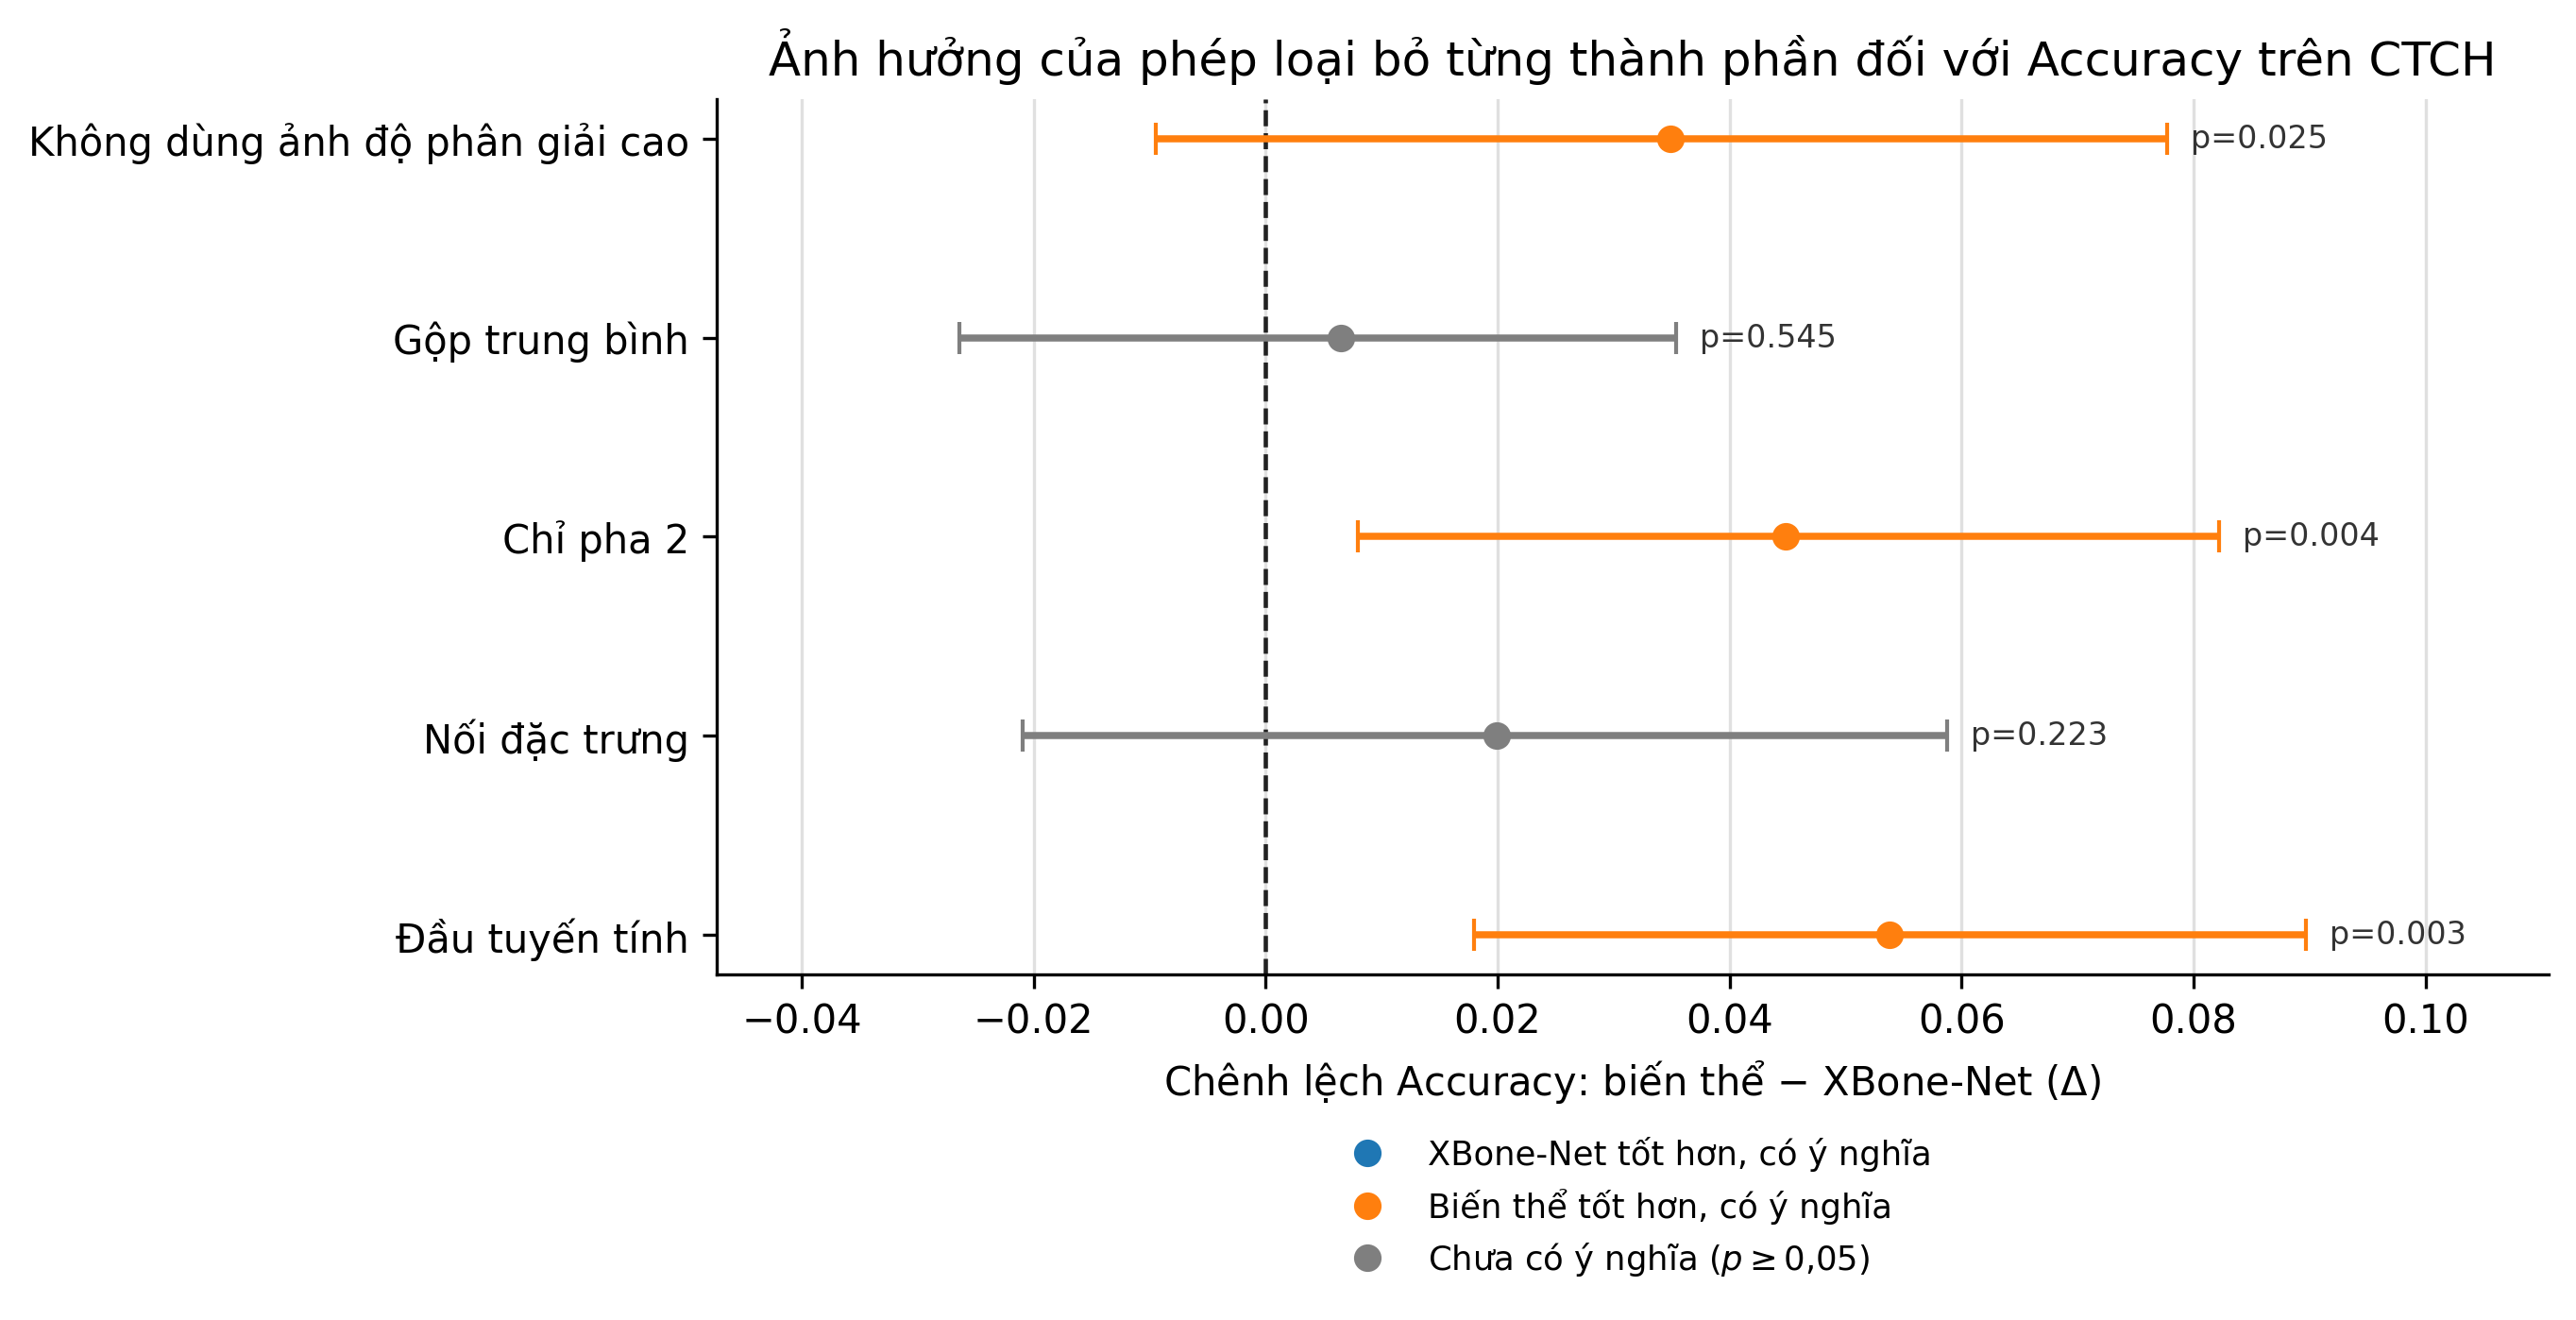
\includegraphics[width=1\linewidth]{generated/chapter4_results/forest_accuracy.png}
\caption{Chênh lệch độ chính xác giữa các biến thể loại bỏ thành phần và XBone-Net trên CTCH}
\label{fig:ablation_accuracy_forest}
\end{figure}

\begin{figure}[H]
\centering
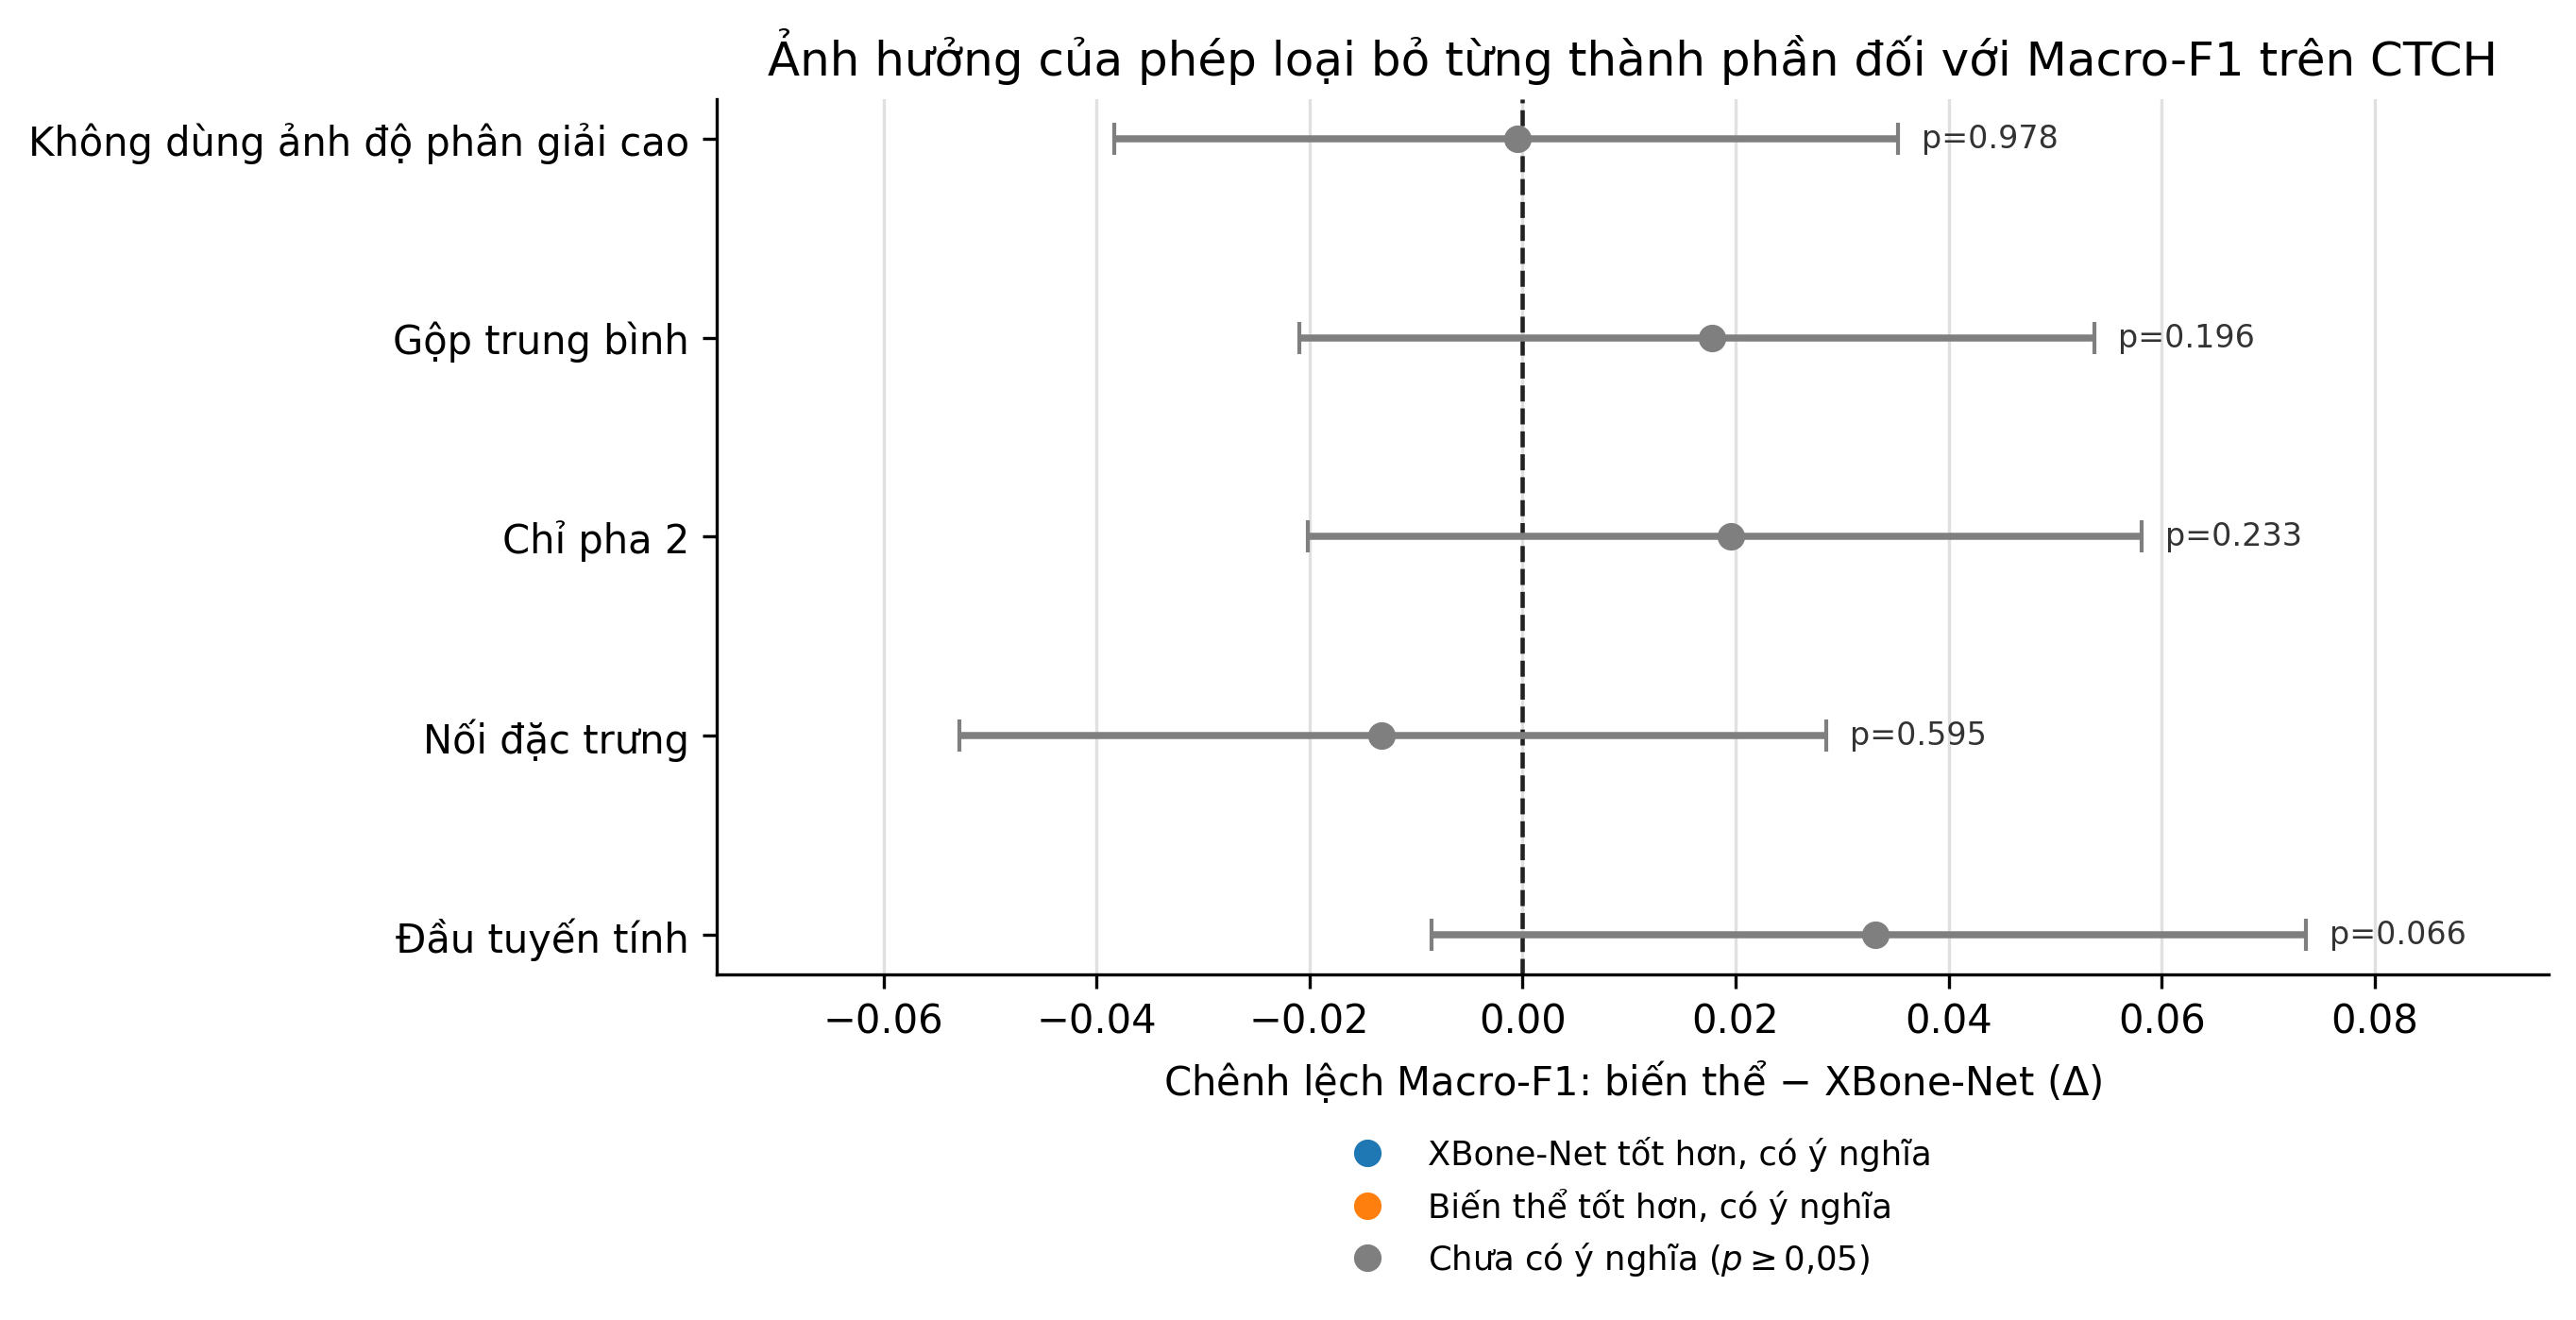
\includegraphics[width=1\linewidth]{generated/chapter4_results/forest_f1_macro.png}
\caption{Chênh lệch điểm Macro-F1 giữa các biến thể và XBone-Net trên CTCH}
\label{fig:ablation_f1_forest}
\end{figure}

\begin{figure}[H]
\centering
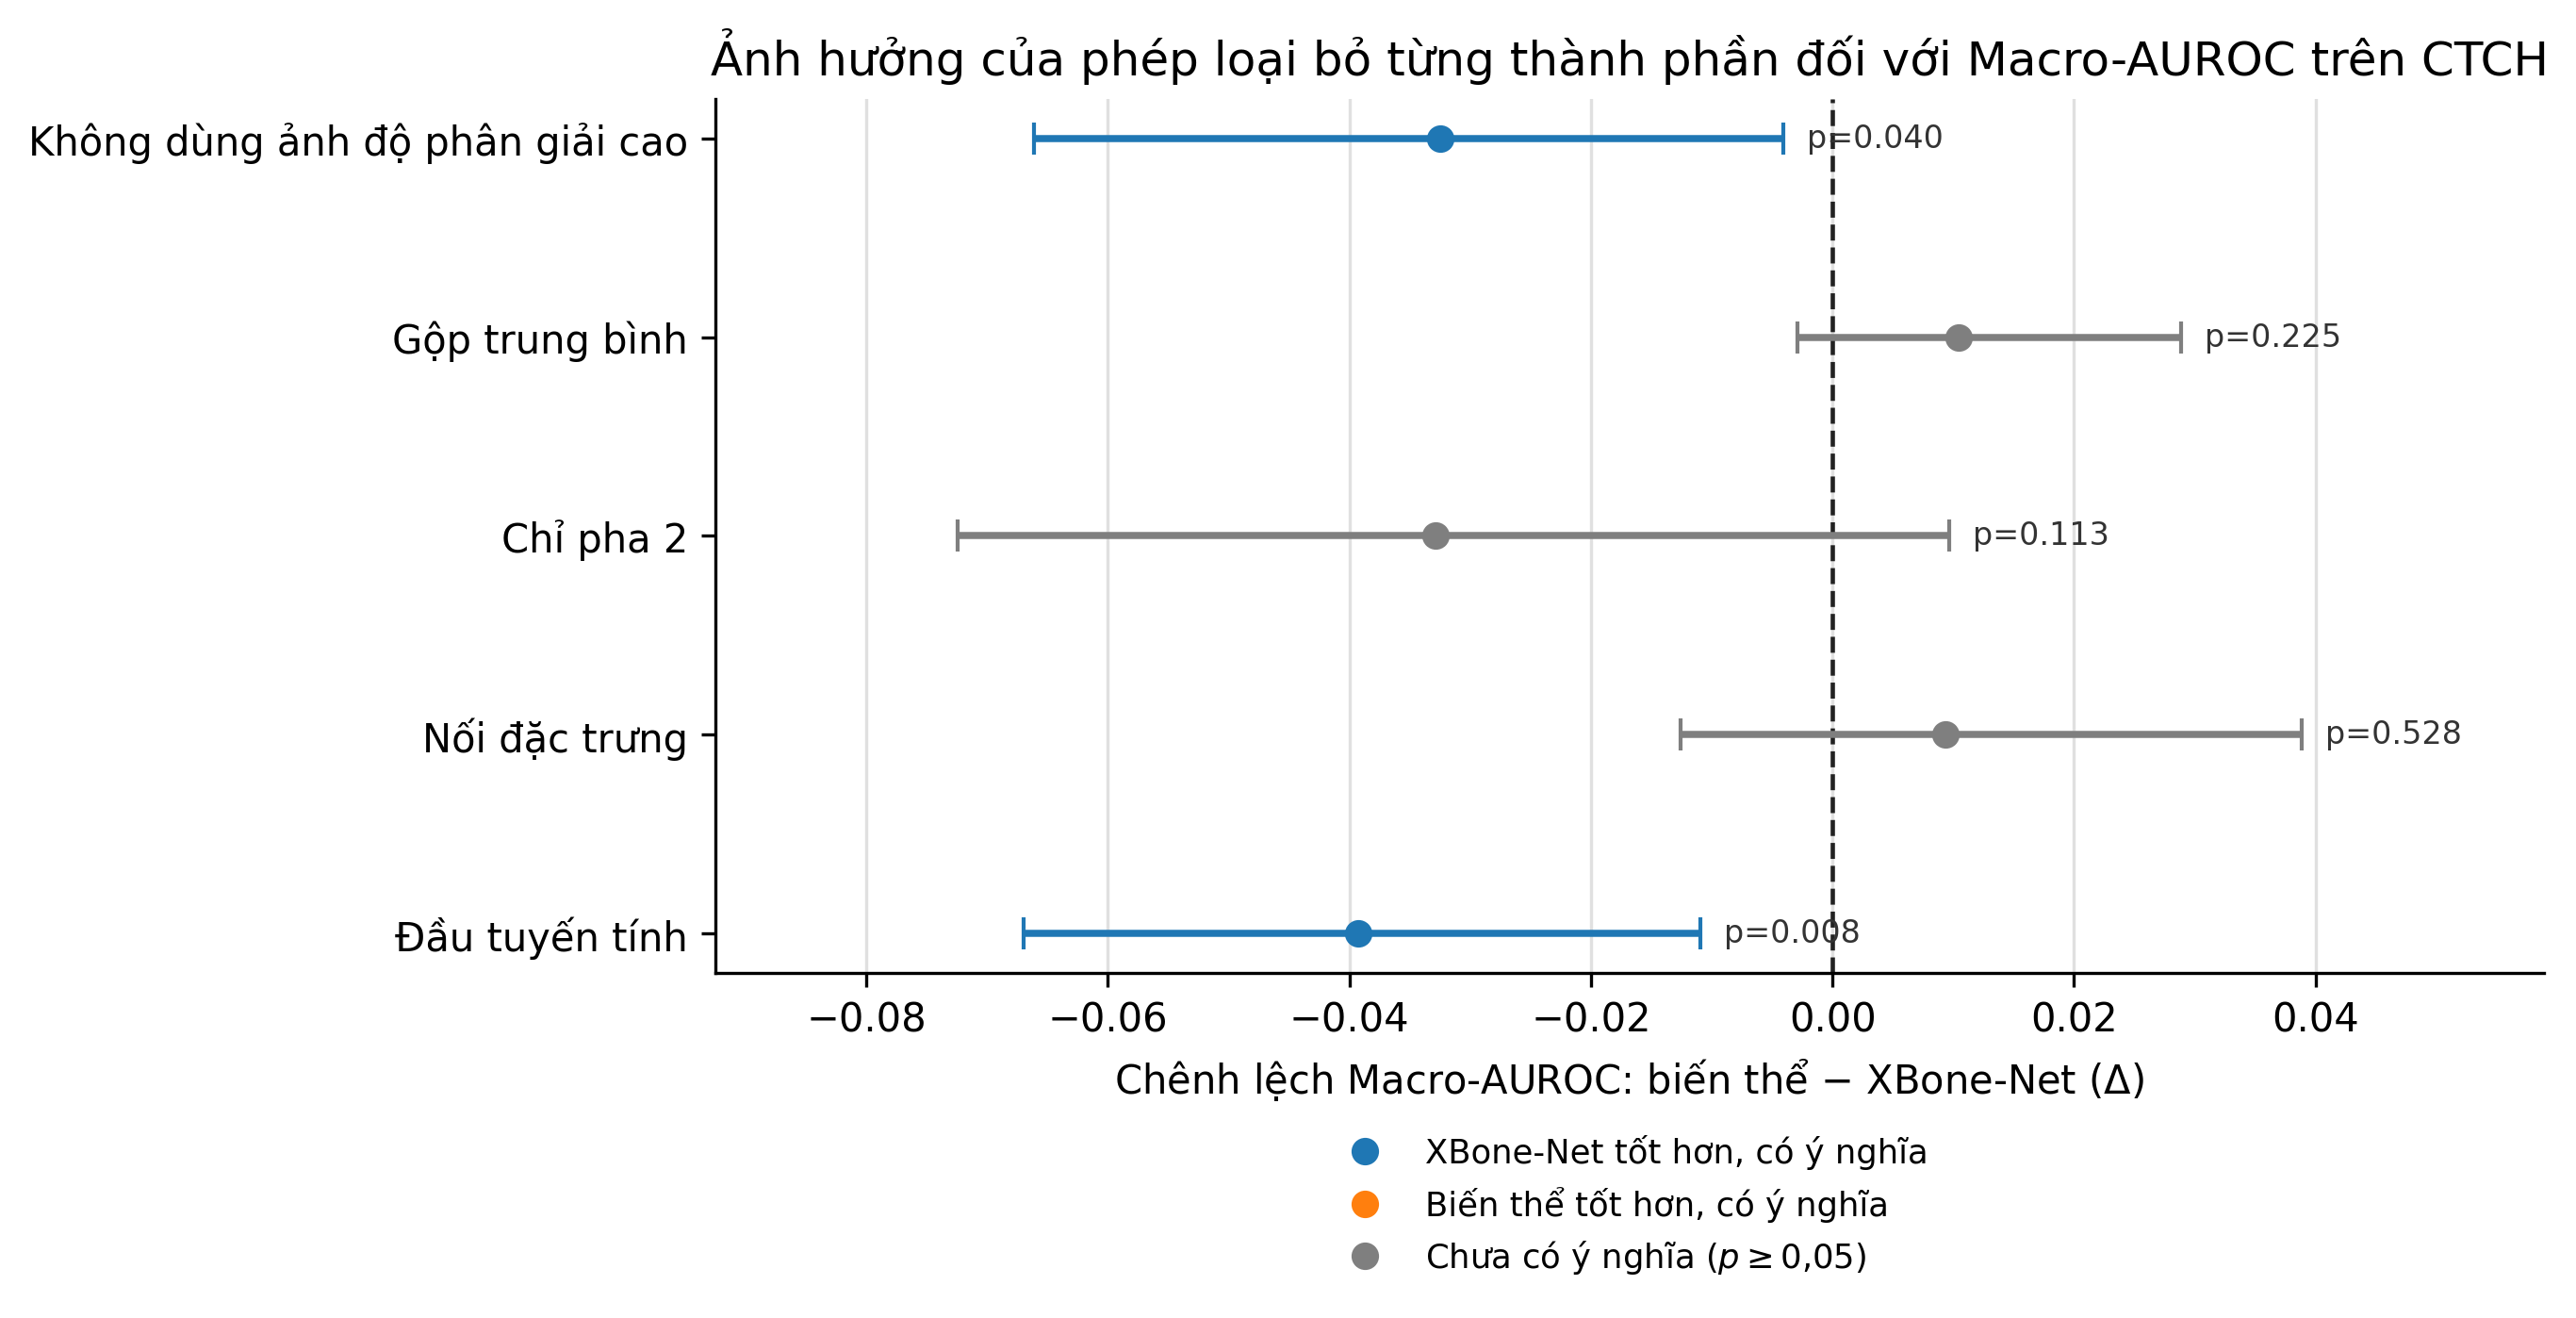
\includegraphics[width=1\linewidth]{generated/chapter4_results/forest_auroc_macro.png}
\caption{Chênh lệch Macro-AUROC giữa các biến thể và XBone-Net trên CTCH}
\label{fig:ablation_auroc_forest}
\end{figure}

\subsection{Đối chứng bổ sung theo nhóm thành phần}

Bên cạnh năm phép loại bỏ chính, Bảng \ref{tab:group_ablation} dưới đây tổng hợp các cấu hình theo bốn nhóm gồm mã hóa ảnh, quy trình huấn luyện, dung hợp và đầu phân loại. Việc đặt các cấu hình trong cùng bảng giúp đối chiếu đồng thời điểm F1 trung bình theo lớp, chất lượng xếp hạng và sai số hiệu chỉnh, thay vì kết luận từ một độ đo riêng lẻ.

\begin{table}[H]
\centering
\scriptsize
\setlength{\tabcolsep}{3.5pt}
\renewcommand{\arraystretch}{1.10}
\resizebox{\textwidth}{!}{%
\begin{tabular}{|l|l|c|c|c|c|}
\hline
\textbf{Nhóm} & \textbf{Cấu hình} &
\textbf{Macro-F1 $\uparrow$} & \textbf{Macro-AUROC $\uparrow$} &
\textbf{Macro-AUPRC $\uparrow$} & \textbf{ECE $\downarrow$} \\ \hline
Tham chiếu & \cellcolor{gray!12}XBone-Net &
\cellcolor{gray!12}$0{.}5558\pm0{.}0072$ &
\cellcolor{gray!12}$0{.}9473\pm0{.}0246$ &
\cellcolor{gray!12}$0{.}6189\pm0{.}0145$ &
\cellcolor{gray!12}$0{.}1032\pm0{.}0303$ \\ \hline
\multirow{4}{*}{Mã hóa ảnh}
& Không xử lý ảnh độ phân giải cao & $0{.}5553\pm0{.}0136$ & $0{.}9148\pm0{.}0223$ & $0{.}5990\pm0{.}0073$ & $0{.}1743\pm0{.}0634$ \\ \cline{2-6}
& Gộp trung bình & $0{.}5736\pm0{.}0251$ & $0{.}9577\pm0{.}0082$ & $0{.}6312\pm0{.}0277$ & $0{.}1506\pm0{.}0564$ \\ \cline{2-6}
& Giảm số đơn vị cục bộ & $0{.}5684\pm0{.}0131$ & $0{.}9442\pm0{.}0241$ & $0{.}6304\pm0{.}0296$ & $0{.}1888\pm0{.}0319$ \\ \cline{2-6}
& Đệm biên giữ tỷ lệ & $0{.}5621\pm0{.}0083$ & $0{.}9340\pm0{.}0284$ & $0{.}6061\pm0{.}0199$ & $0{.}1934\pm0{.}0403$ \\ \hline
\multirow{2}{*}{Huấn luyện}
& Chỉ pha 2 & $0{.}5753\pm0{.}0175$ & $0{.}9144\pm0{.}0198$ & $0{.}6268\pm0{.}0170$ & $0{.}1868\pm0{.}0724$ \\ \cline{2-6}
& Hợp nhất pha 1 & $0{.}5401\pm0{.}0303$ & $0{.}9513\pm0{.}0166$ & $0{.}5903\pm0{.}0152$ & $0{.}1664\pm0{.}0440$ \\ \hline
\multirow{3}{*}{Dung hợp}
& Nối đặc trưng & $0{.}5425\pm0{.}0130$ & $0{.}9566\pm0{.}0046$ & $0{.}6019\pm0{.}0139$ & $\mathbf{0{.}0789\pm0{.}0148}$ \\ \cline{2-6}
& Ảnh truy vấn văn bản & $0{.}5559\pm0{.}0159$ & $0{.}9449\pm0{.}0268$ & $0{.}6174\pm0{.}0292$ & $0{.}1782\pm0{.}0108$ \\ \cline{2-6}
& Văn bản truy vấn ảnh & $0{.}5632\pm0{.}0217$ & $0{.}9410\pm0{.}0216$ & $0{.}6211\pm0{.}0137$ & $0{.}1299\pm0{.}0568$ \\ \hline
\multirow{3}{*}{Đầu phân loại}
& Đầu tuyến tính & $\mathbf{0{.}5889\pm0{.}0251}$ & $0{.}9080\pm0{.}0099$ & $0{.}6076\pm0{.}0218$ & $0{.}0882\pm0{.}0153$ \\ \cline{2-6}
& Không trọng số lớp & $0{.}5641\pm0{.}0093$ & $\mathbf{0{.}9528\pm0{.}0056}$ & $0{.}6133\pm0{.}0114$ & $0{.}1286\pm0{.}0423$ \\ \cline{2-6}
& Không độ chệch theo lớp & $0{.}5740\pm0{.}0126$ & $0{.}9355\pm0{.}0188$ & $0{.}6125\pm0{.}0116$ & $0{.}1281\pm0{.}0519$ \\ \hline
\end{tabular}%
}
\caption*{Đối chứng theo nhóm thành phần phục vụ RQ2 trên CTCH}
\end{table}


Trong nhóm mã hóa ảnh, giảm số đơn vị cục bộ và đệm biên giữ tỷ lệ làm điểm F1 tăng lần lượt lên $0{,}5684\pm0{,}0131$ và $0{,}5621\pm0{,}0083$, nhưng ECE đều tăng lên trên $0{,}18$. Gộp trung bình đạt Macro-AUROC và Macro-AUPRC cao nhất trong nhóm, song ECE tăng từ $0{,}1032\pm0{,}0303$ lên $0{,}1506\pm0{,}0564$. Các kết quả này củng cố nhận định rằng việc duy trì thông tin cục bộ có ích cho một số mục tiêu, nhưng số vùng và cơ chế gộp hiện tại chưa phải lựa chọn tối ưu đồng thời cho quyết định lớp, xếp hạng và hiệu chỉnh.

Trong nhóm huấn luyện, chỉ pha 2 làm điểm F1 và Macro-AUPRC tăng nhưng làm Macro-AUROC giảm và ECE tăng. Hợp nhất pha 1 đạt Macro-AUROC $0{,}9513\pm0{,}0166$ nhưng thấp hơn cấu hình đầy đủ về điểm F1 và Macro-AUPRC. Trong nhóm dung hợp, hai hướng chú ý một chiều đạt điểm F1 lần lượt $0{,}5559\pm0{,}0159$ và $0{,}5632\pm0{,}0217$, gần cấu hình hai chiều $0{,}5558\pm0{,}0072$, nhưng không hướng nào cải thiện đồng thời mọi độ đo. Phép nối đặc trưng có Macro-AUROC và ECE thuận lợi hơn nhưng điểm F1 thấp hơn. Ở nhóm đầu phân loại, đầu tuyến tính đạt điểm F1 cao nhất, còn bỏ trọng số lớp đạt Macro-AUROC cao nhất. Cả hai đều tạo đánh đổi ở các độ đo còn lại.

\subsection{Tổng kết}
Nhánh ảnh cục bộ, huấn luyện hai pha, cơ chế dung hợp và đầu phân lớp theo tâm lớp đều làm thay đổi ít nhất một trong ba khía cạnh gồm quyết định lớp, chất lượng xếp hạng và hiệu chỉnh, nhưng không thành phần nào cải thiện nhất quán toàn bộ tiêu chí. Cấu hình đầy đủ vì vậy được xem là một điểm đánh đổi: nhánh cục bộ và pha khớp ngữ nghĩa có liên hệ với chất lượng xếp hạng hoặc hiệu chỉnh, trong khi gộp trung bình, đầu tuyến tính và một số biến thể đơn giản đạt điểm F1 hoặc độ chính xác cao hơn. Kết quả gần nhau giữa chú ý chéo hai chiều và hai hướng chú ý một chiều cũng cho thấy cơ chế dung hợp hiện tại có thể được đơn giản hóa.

\section{Biểu diễn và dữ liệu ngoài phân phối}
\label{sec:representation_ood}

\subsection{Hình học biểu diễn}
\label{subsec:representation_geometry}
Nhằm khảo sát cấu trúc hình học được hình thành trong XBone-Net, sáu không gian biểu diễn được đánh giá trên 669 mẫu kiểm thử CTCH bằng chỉ số Silhouette và Davies--Bouldin. Các chỉ số định lượng được tính trong không gian biểu diễn đầy đủ, còn phép chiếu PCA hai chiều chỉ được sử dụng để minh họa trực quan.

\begin{table}[htbp]
\centering
\resizebox{\textwidth}{!}{%
\begin{tabular}{|l|c|c|}
\hline
Không gian biểu diễn & Silhouette $\uparrow$ & Davies--Bouldin $\downarrow$ \\ \hline
Dung hợp & $\mathbf{-0{.}0075\pm0{.}0325}$ & $\mathbf{2{.}8672\pm0{.}0719}$ \\ \hline
Ảnh toàn cục & $-0{.}0974\pm0{.}0197$ & $4{.}1912\pm0{.}0453$ \\ \hline
Tóm tắt ảnh cục bộ & $-0{.}1595\pm0{.}0284$ & $4{.}3243\pm0{.}2035$ \\ \hline
Văn bản toàn cục & $-0{.}1205\pm0{.}0104$ & $3{.}6686\pm0{.}0914$ \\ \hline
Ảnh nhận ngữ cảnh văn bản & $-0{.}0880\pm0{.}0124$ & $3{.}7898\pm0{.}0989$ \\ \hline
Văn bản nhận ngữ cảnh ảnh & $-0{.}1179\pm0{.}0115$ & $3{.}5628\pm0{.}1281$ \\ \hline
\end{tabular}%
}
\caption{Hình học của các không gian biểu diễn trên 669 mẫu kiểm thử CTCH theo Silhouette và Davies-Bouldin}
\label{tab:explain_representation}
\end{table}


Bảng~\ref{tab:explain_representation} cho thấy biểu diễn dung hợp đạt Silhouette $-0{,}0075\pm0{,}0325$ và Davies--Bouldin $2{,}8672\pm0{,}0719$, là kết quả thuận lợi nhất trong sáu không gian được khảo sát. Biểu diễn ảnh sau khi nhận ngữ cảnh văn bản đứng thứ hai về Silhouette với $-0{,}0880\pm0{,}0124$, trong khi biểu diễn văn bản sau khi nhận ngữ cảnh ảnh đứng thứ hai về Davies--Bouldin với $3{,}5628\pm0{,}1281$. Tóm tắt ảnh cục bộ có Silhouette thấp nhất $-0{,}1595\pm0{,}0284$ và Davies--Bouldin cao nhất $4{,}3243\pm0{,}2035$.

Tất cả giá trị Silhouette đều âm hoặc gần 0, cho thấy các lớp vẫn chồng lấn đáng kể và chưa hình thành những cụm tách biệt ổn định. Vì vậy, kết quả chỉ hỗ trợ kết luận rằng dung hợp tạo cấu trúc lớp thuận lợi hơn một cách tương đối so với các không gian còn lại. Kết quả không chứng minh rằng 22 lớp CTCH đã được phân tách rõ ràng.

\begin{figure}[H]
\centering
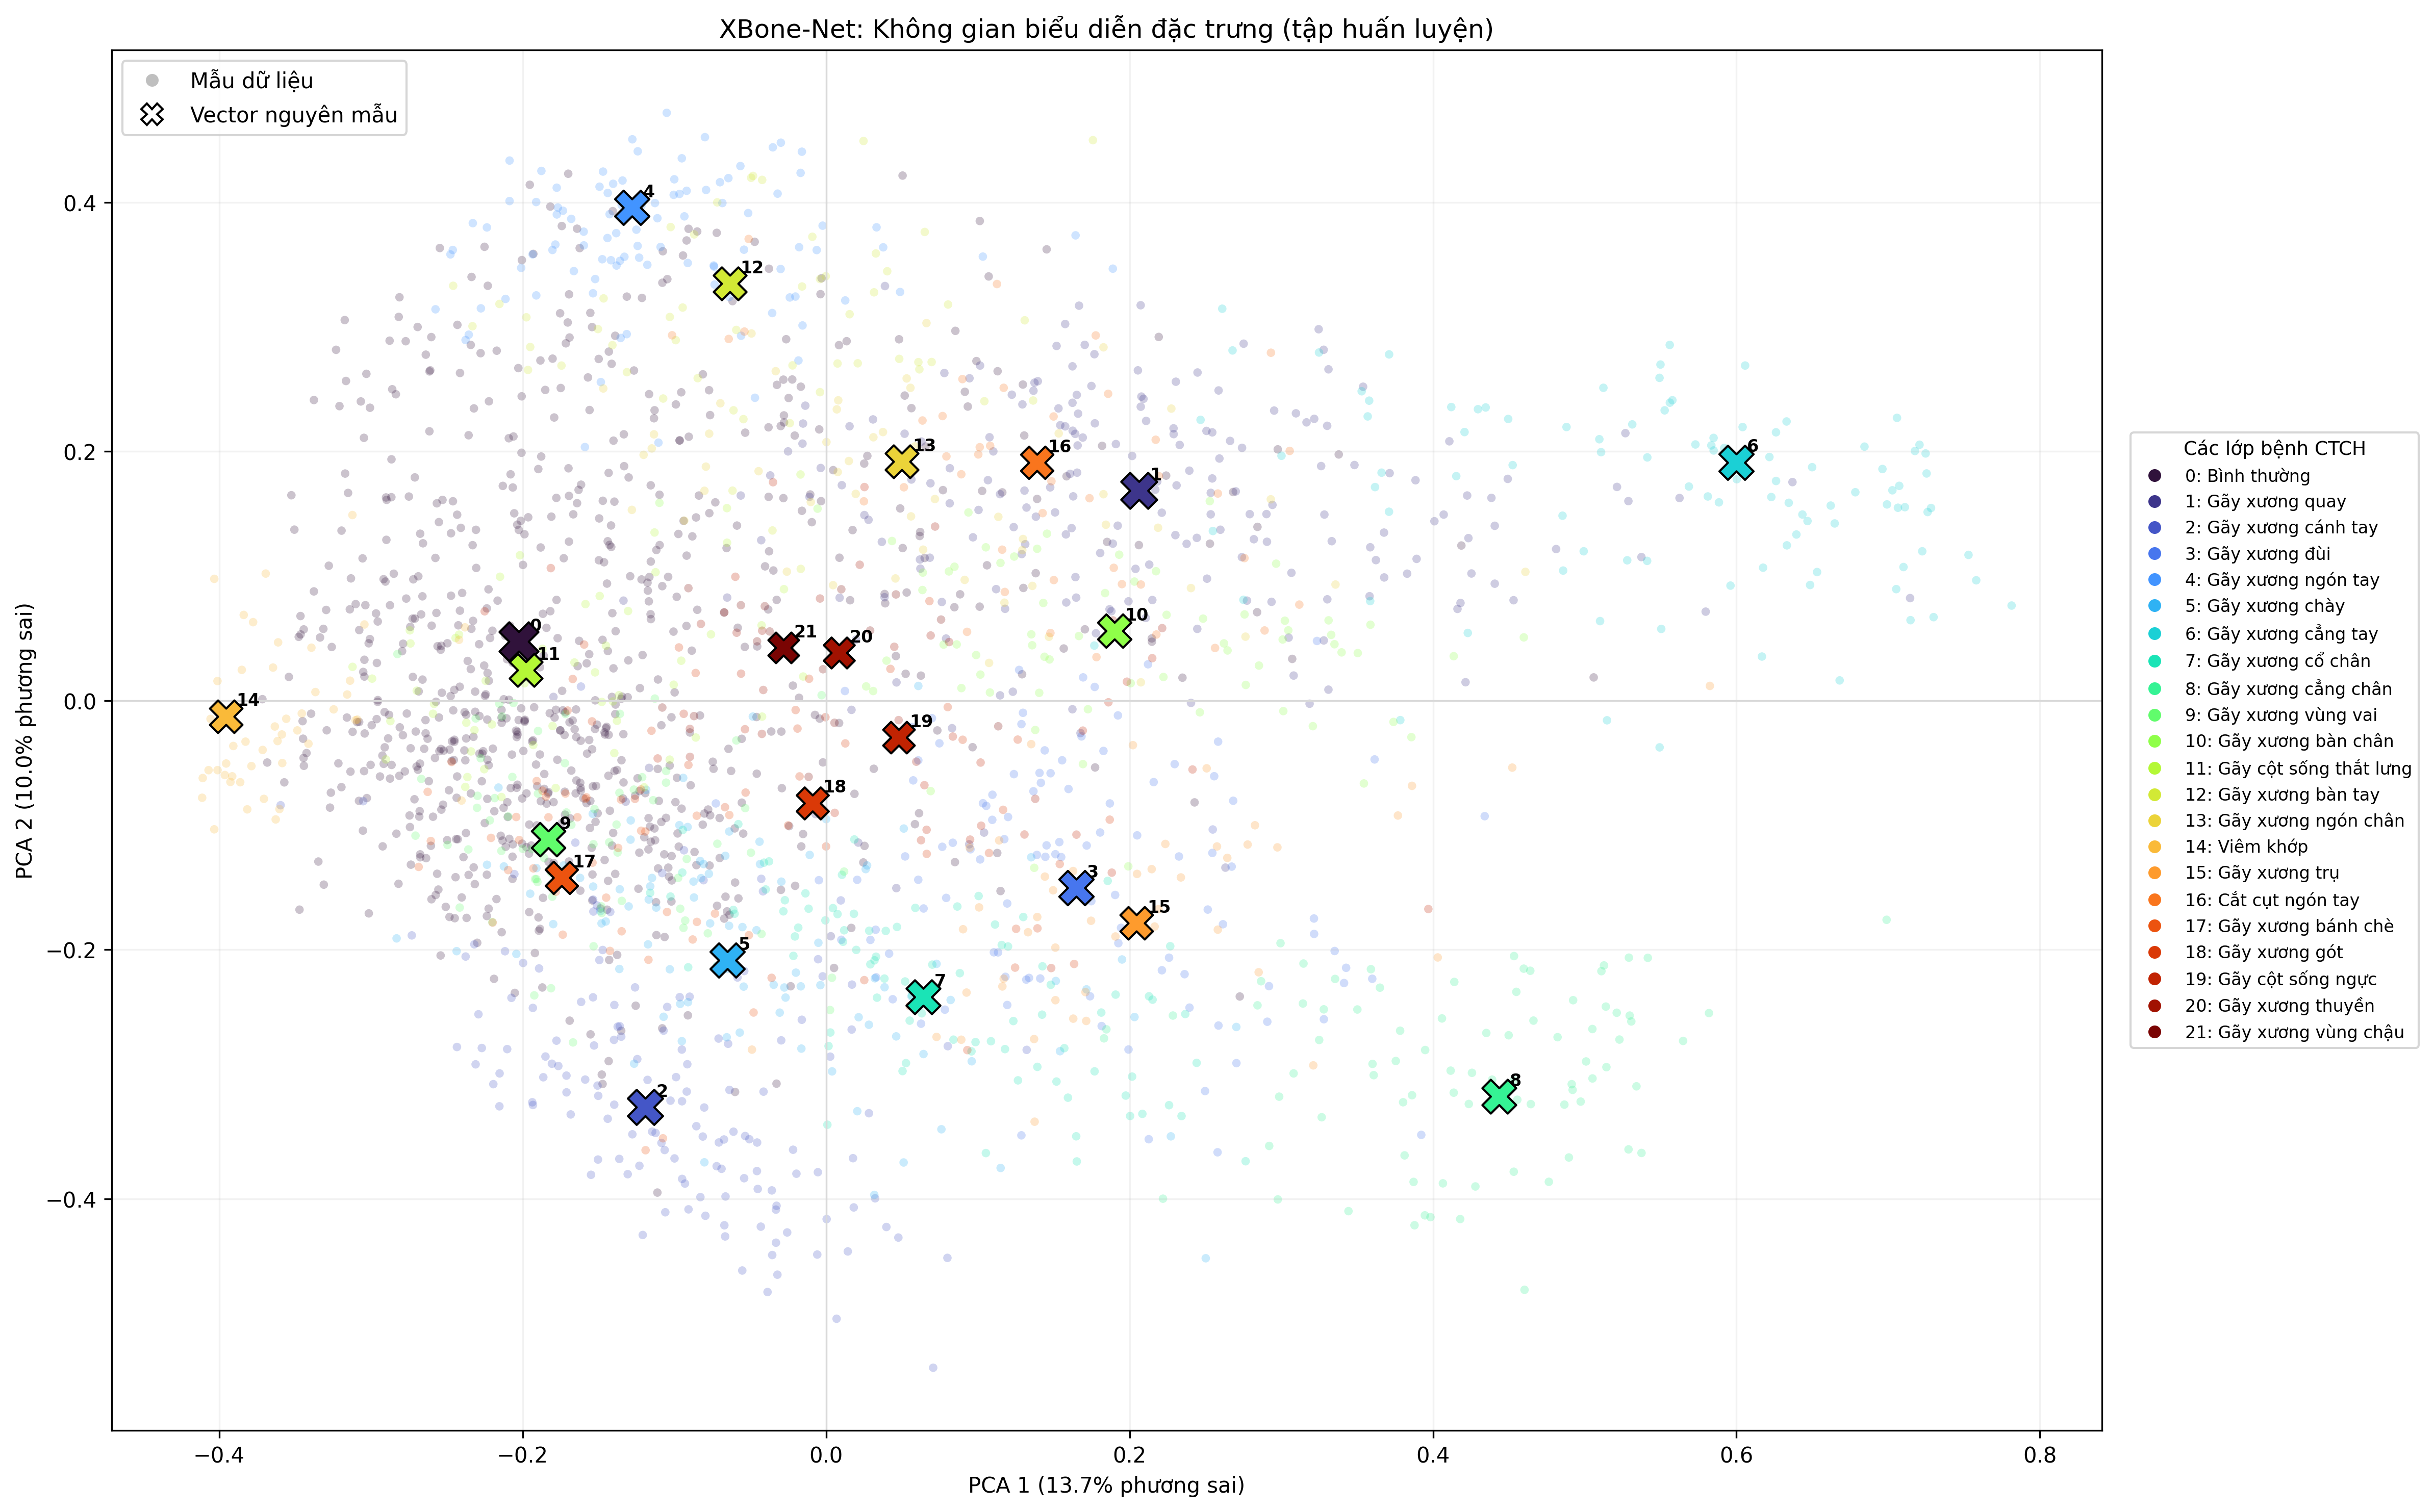
\includegraphics[width=1\linewidth]{generated/chapter4_results/centroid_projection.png}
\caption{Phép chiếu PCA hai chiều của biểu diễn dung hợp trên các mẫu huấn luyện CTCH và các tâm lớp thực nghiệm được ước lượng từ tập huấn luyện}
\label{fig:centroid_projection}
\end{figure}

Hình~\ref{fig:centroid_projection} cho thấy các mẫu huấn luyện của nhiều lớp vẫn chồng lấn đáng kể trong phép chiếu hai chiều, mặc dù một số tâm lớp phân bố theo các hướng khác nhau. Phép PCA được khớp một lần trên các biểu diễn huấn luyện đã chuẩn hóa cùng các tâm lớp. Các biểu diễn thuộc tập xác thực, tập kiểm thử hoặc tập OOD chỉ được biến đổi bằng phép chiếu đã khớp này, không được dùng để xác định lại các trục PCA. Một số tâm không trùng với vùng mật độ lớn của các điểm cùng lớp, có thể phản ánh mất cân bằng lớp, cấu trúc đa đỉnh hoặc sự méo khoảng cách do phép chiếu chỉ giữ một phần phương sai. Vì vậy, hình chỉ mô tả cấu trúc của không gian tham chiếu huấn luyện. Khoảng cách trên mặt phẳng PCA không thay thế độ tương đồng cosine hoặc khoảng cách Mahalanobis trong không gian biểu diễn đầy đủ.

\subsection{Phát hiện dữ liệu ngoài phân phối}
\label{subsec:ood_detection_results}
Bảng~\ref{tab:ood_semantic_btxrd} đánh giá bốn điểm OOD trên 669 mẫu CTCH trong phân phối, 44 mẫu ngoài không gian nhãn nhưng cùng nguồn CTCH và 750 mẫu BTXRD. Nhóm 44 mẫu là kịch bản gần miền và có quy mô nhỏ, trong khi BTXRD đồng thời thay đổi nguồn ảnh, nguồn văn bản và không gian nhãn.

\begin{table}[htbp]
\centering
\small
\resizebox{\textwidth}{!}{%
\begin{tabular}{|l|l|c|c|c|}
\hline
\multicolumn{1}{|c|}{\textbf{Kịch bản}} & \multicolumn{1}{c|}{\textbf{Phương pháp}} & \multicolumn{1}{c|}{\textbf{AUROC-OOD $\uparrow$}} & \multicolumn{1}{c|}{\textbf{AUPR-Out $\uparrow$}} & \multicolumn{1}{c|}{\textbf{FPR@95\%TPR $\downarrow$}} \\ \hline
\multirow{4}{*}{Semantic OOD} & Cosine-centroid & $0.5739\pm0.0185$ & $0.0595\pm0.0024$ & $\mathbf{0.8966\pm0.0345}$ \\ \cline{2-5}
 & Mahalanobis-centroid & $\mathbf{0.5840\pm0.0203}$ & $0.0553\pm0.0028$ & $0.9195\pm0.0527$ \\ \cline{2-5}
 & kNN & $0.5781\pm0.0289$ & $0.0608\pm0.0034$ & $0.9310\pm0.0345$ \\ \cline{2-5}
 & Entropy & $0.5332\pm0.0323$ & $\mathbf{0.0634\pm0.0204}$ & $0.9195\pm0.0398$ \\ \hline
\multirow{4}{*}{BTXRD} & Cosine-centroid & $0.7301\pm0.0850$ & $0.7268\pm0.0633$ & $0.7956\pm0.0575$ \\ \cline{2-5}
 & Mahalanobis-centroid & $\mathbf{0.8042\pm0.0938}$ & $\mathbf{0.8009\pm0.0609}$ & $\mathbf{0.7071\pm0.0678}$ \\ \cline{2-5}
 & kNN & $0.7725\pm0.0970$ & $0.7641\pm0.0703$ & $0.7671\pm0.0963$ \\ \cline{2-5}
 & Entropy & $0.6918\pm0.0859$ & $0.7033\pm0.0731$ & $0.8258\pm0.0697$ \\ \hline
\end{tabular}
}
\caption{Kết quả phát hiện OOD hậu xử lý của XBone-Net trên các kịch bản được xét; các giá trị được trình bày dưới dạng trung bình $\pm$ độ lệch chuẩn trên ba seed.}
\label{tab:ood_semantic_btxrd}
\end{table}


Trong bốn phương pháp, khoảng cách Mahalanobis đạt AUROC-OOD cao nhất trên tập kiểm thử BTXRD với $0{,}8042\pm0{,}0938$ và trên nhóm ngoài không gian nhãn với $0{,}6286\pm0{,}0177$. Phương pháp năm láng giềng gần nhất đạt AUPR-Out cao nhất trên nhóm ngoài không gian nhãn. Các kết quả cho thấy biểu diễn chứa tín hiệu dịch chuyển, nhưng mức phân biệt phụ thuộc mạnh vào dạng OOD được xét.

Bảng~\ref{tab:rq4_ood_baselines} giữ cố định điểm Mahalanobis để so sánh ảnh hưởng của không gian biểu diễn. BiomedCLIP không mẫu đạt AUROC-OOD $0{,}6362$ trên nhóm ngoài không gian nhãn trong một lần đánh giá, cao hơn nhẹ XBone-Net. Tuy nhiên, XBone-Net đạt AUPR-Out cao nhất trong nhóm các biểu diễn được huấn luyện trên kịch bản này. Trên BTXRD, phép nối đặc trưng dẫn đầu cả ba độ đo với AUROC-OOD $0{,}8966\pm0{,}0478$ và FPR@95\%TPR $0{,}5978\pm0{,}1744$. Kết quả cho thấy kiến trúc dung hợp phức tạp không mặc nhiên tạo không gian biểu diễn tốt nhất cho mọi dạng dịch chuyển.

\begin{table}[htbp]
\centering
\resizebox{\columnwidth}{!}{%
\begin{tabular}{|c|l|c|c|c|}
\hline
\textbf{Kịch bản} &
  \multicolumn{1}{c|}{\textbf{Biểu diễn}} &
  \textbf{AUROC-OOD $\uparrow$} &
  \textbf{AUPR-Out $\uparrow$} &
  \textbf{FPR@95\%TPR $\downarrow$} \\ \hline
\multirow{4}{*}{\begin{tabular}[c]{@{}c@{}}OOD \\ CTCH\end{tabular}} &
  XBone-Net &
  $\mathbf{0{.}6286\pm0{.}0177}$ &
  $\mathbf{0{.}1034\pm0{.}0092}$ &
  $\mathbf{0{.}8864\pm0{.}0394}$ \\ \cline{2-5} 
                       & Chỉ pha 2      & $0{.}5921\pm0{.}0535$          & $0{.}0870\pm0{.}0190$          & $0{.}9242\pm0{.}0262$          \\ \cline{2-5} 
                       & Nối đặc trưng  & $0{.}5795\pm0{.}0151$          & $0{.}0980\pm0{.}0151$          & $0{.}9015\pm0{.}0131$          \\ \cline{2-5} 
                       & Đầu tuyến tính & $0{.}5464\pm0{.}0336$          & $0{.}0746\pm0{.}0079$          & $0{.}9545\pm0{.}0394$          \\ \hline
\multirow{4}{*}{BTXRD} & XBone-Net      & $0{.}8042\pm0{.}0938$          & $0{.}8009\pm0{.}0609$          & $0{.}7071\pm0{.}0678$          \\ \cline{2-5} 
                       & Chỉ pha 2      & $0{.}6723\pm0{.}0332$          & $0{.}7015\pm0{.}0382$          & $0{.}8133\pm0{.}0501$          \\ \cline{2-5} 
                       & Nối đặc trưng  & $\mathbf{0{.}8966\pm0{.}0478}$ & $\mathbf{0{.}8713\pm0{.}0555}$ & $\mathbf{0{.}5978\pm0{.}1744}$ \\ \cline{2-5} 
                       & Đầu tuyến tính & $0{.}6517\pm0{.}0651$          & $0{.}6719\pm0{.}0623$          & $0{.}8382\pm0{.}0584$          \\ \hline
\end{tabular}%
}
\caption{So sánh điểm Mahalanobis giữa các biến thể của XBone-Net}
\label{tab:rq4_ood_baselines}
\end{table}


Hình~\ref{fig:centroid_projection_ood} giữ nguyên hệ trục PCA đã khớp trên tập huấn luyện trong Hình~\ref{fig:centroid_projection}, sau đó chiếu thêm một mẫu OOD vào hệ trục này. Do đó, các điểm nền và tâm lớp trong hình biểu diễn không gian tham chiếu huấn luyện, không phải phân phối dùng để hiệu chỉnh ngưỡng. Vị trí trên mặt phẳng PCA chỉ hỗ trợ quan sát định tính và không được dùng để quyết định mẫu có phải OOD hay không.

Ở hạt giống 42, điểm Mahalanobis của mẫu là $19{,}85$. Trạng thái cảnh báo trong Hình~\ref{fig:ood_sample} được xác định bằng ngưỡng vận hành $\tau_{\mathrm{alert}}=31{,}65$, được hiệu chỉnh trên tập xác thực để giữ lại khoảng $95\%$ mẫu trong phân phối. Vì $19{,}85<31{,}65$, mẫu không bị cảnh báo và được chấp nhận nhầm như dữ liệu trong phân phối. Ngưỡng $\tau_{95}^{\mathrm{test}}=30{,}29$ được xác định riêng trên tập kiểm thử để tính FPR@95\%TPR, nên chỉ phục vụ đánh giá hậu nghiệm và không tham gia quyết định cảnh báo trong hai hình. Mẫu huấn luyện gần nhất theo độ tương đồng cosine thuộc lớp gãy xương cánh tay. Ví dụ này minh họa giới hạn của điểm khoảng cách đối với OOD gần miền.

\begin{figure}[H]
\centering
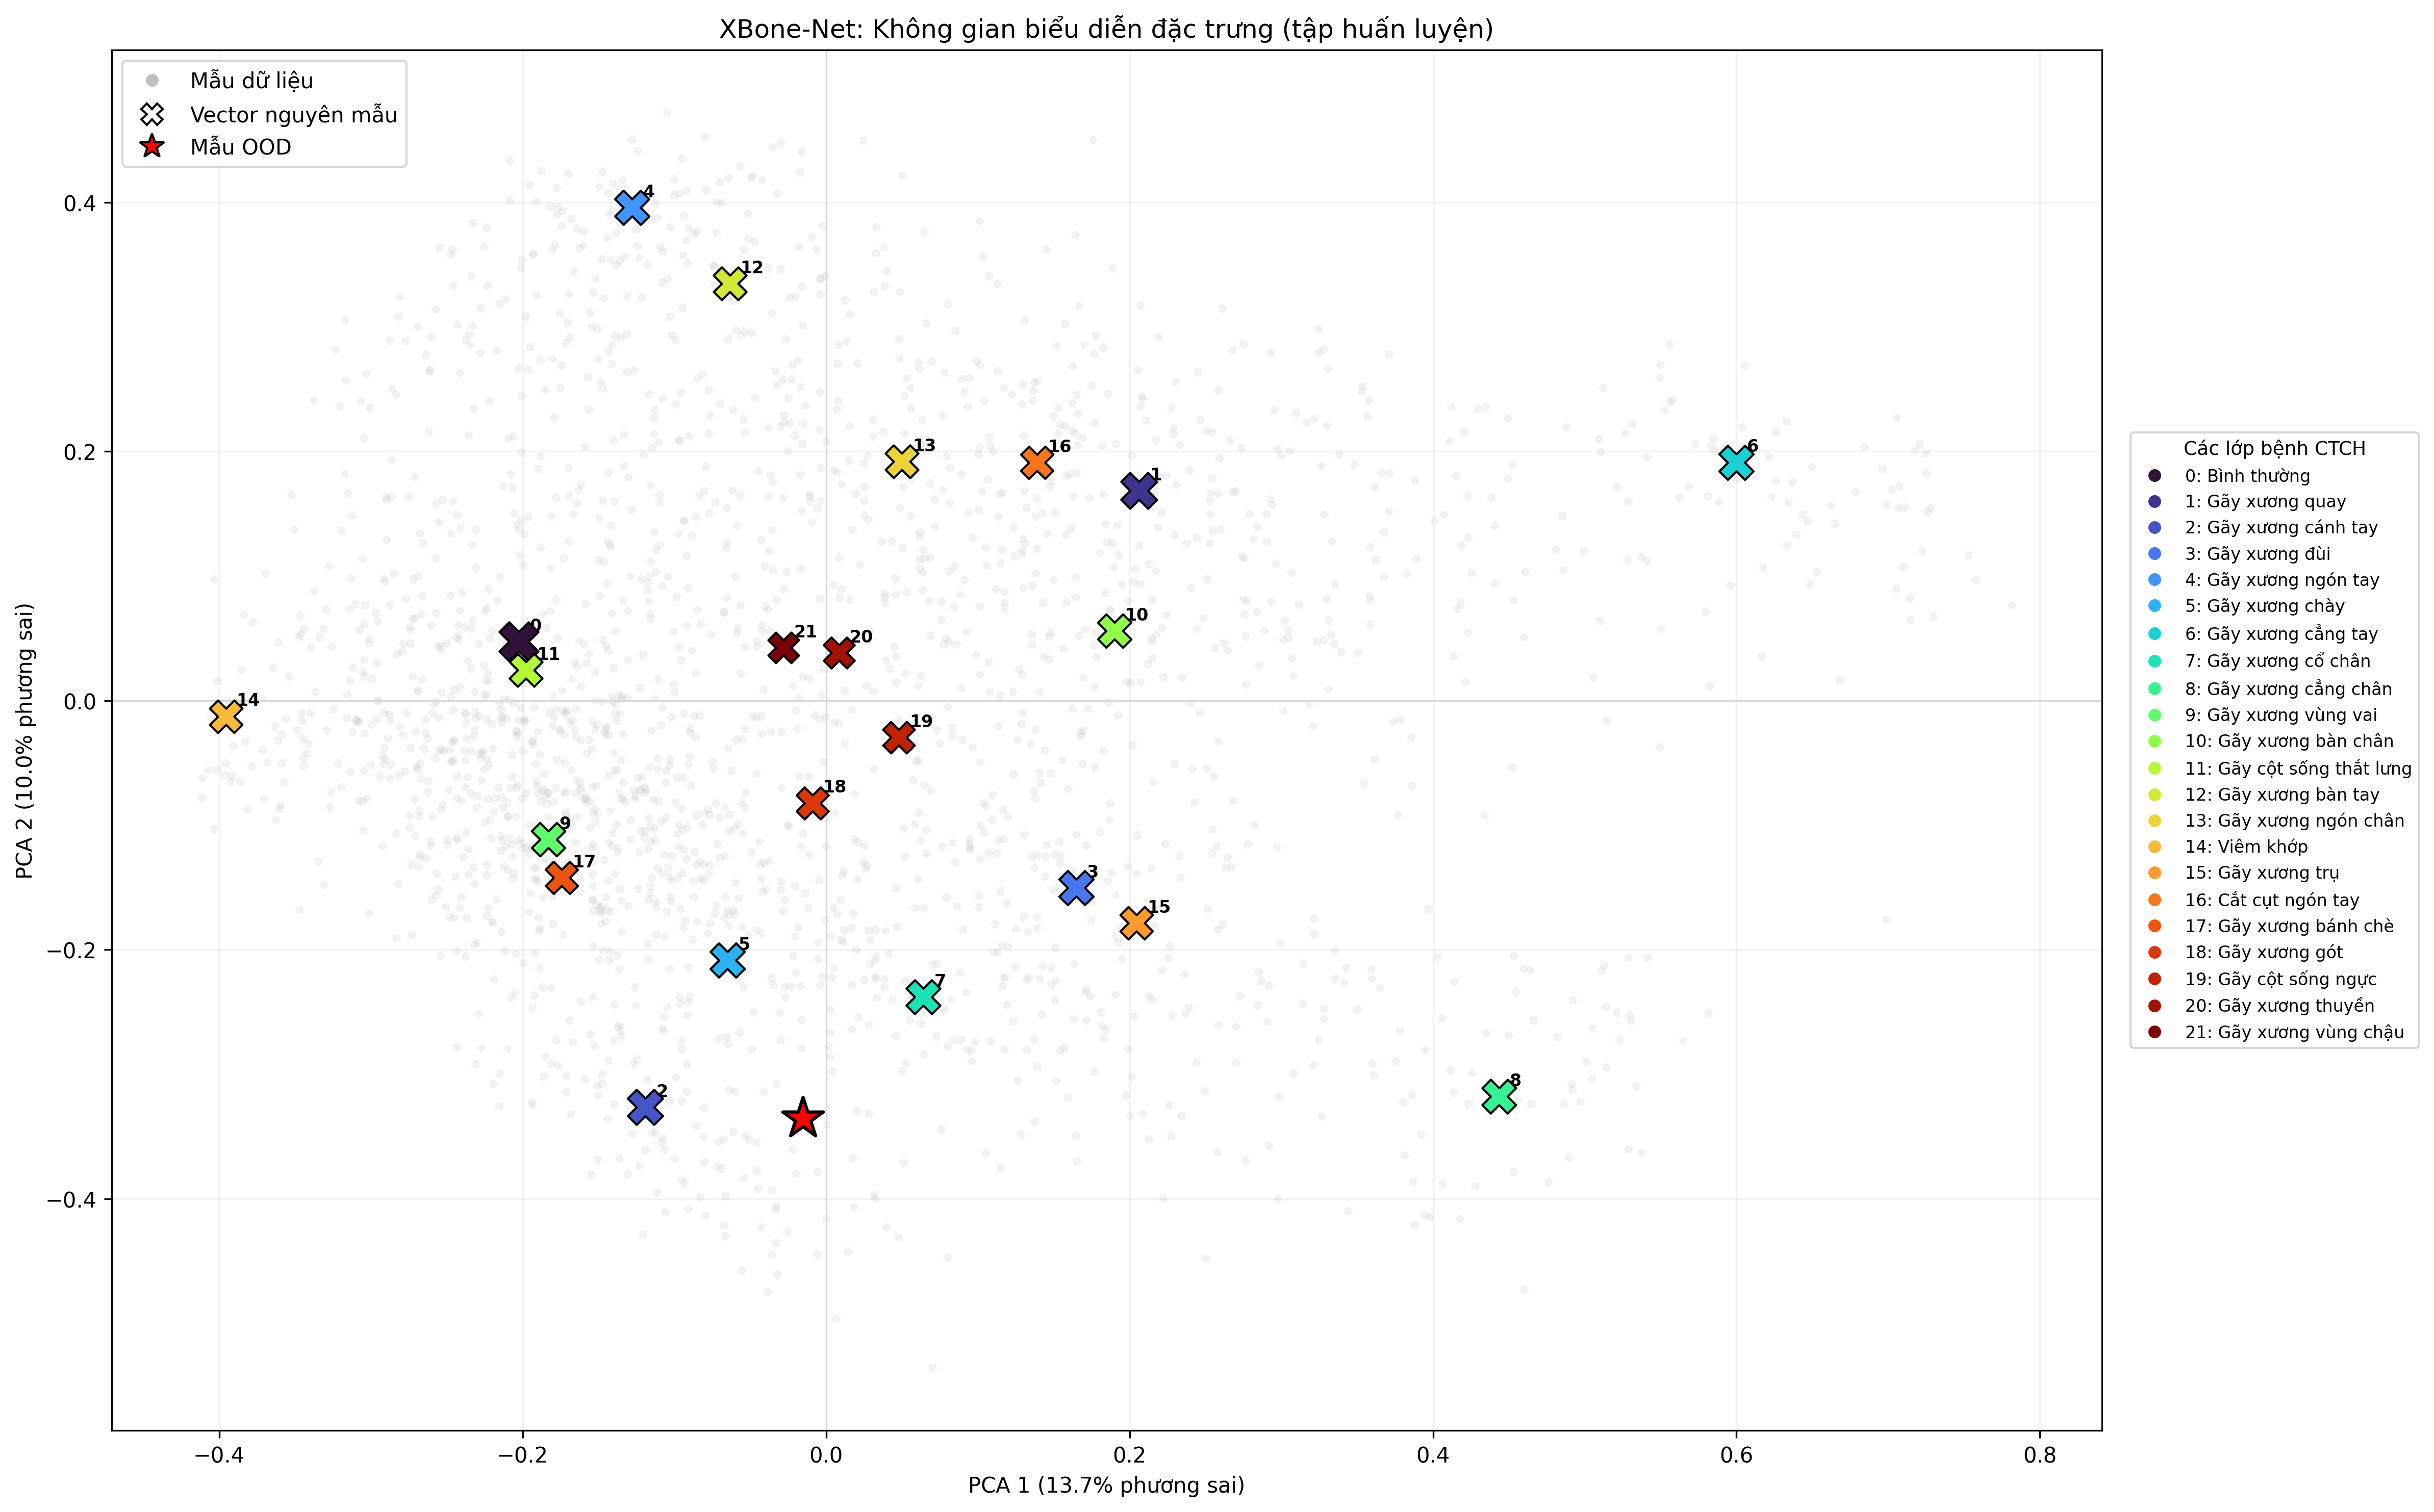
\includegraphics[width=1\linewidth]{generated/chapter4_results/centroid_projection_ood.png}
\caption{Phép chiếu PCA của không gian biểu diễn dung hợp với một mẫu OOD bị chấp nhận nhầm}
\label{fig:centroid_projection_ood}
\end{figure}

\begin{figure}[H]
\centering
\begin{subfigure}[t]{0.36\textwidth}
\centering
\includegraphics[height=0.33\textheight]{../../data/CTCH/images/8_img-01109-00001.jpg}
\caption{Mẫu OOD có điểm Mahalanobis $19{,}85$}
\end{subfigure}
\hfill
\begin{subfigure}[t]{0.36\textwidth}
\centering
\includegraphics[height=0.33\textheight]{../../data/CTCH/images/368_img-00004-00001.jpg}
\caption{Mẫu huấn luyện gần nhất, độ tương đồng cosine $0{,}940$}
\end{subfigure}
\caption{So sánh mẫu OOD bị chấp nhận nhầm tại ngưỡng cảnh báo $\tau_{\mathrm{alert}}=31{,}65$ được hiệu chỉnh trên tập xác thực với mẫu huấn luyện gần nhất trong không gian biểu diễn}
\label{fig:ood_sample}
\end{figure}

\subsection{Tổng kết}
Biểu diễn dung hợp có cấu trúc lớp thuận lợi hơn tương đối trên CTCH và chứa tín hiệu phân biệt dữ liệu ngoài phân phối. Tín hiệu rõ hơn khi nguồn ảnh, nguồn văn bản và không gian nhãn cùng thay đổi như trong kịch bản BTXRD, nhưng yếu đối với các bệnh ngoài không gian nhãn còn gần miền CTCH. Do FPR@95\%TPR còn cao ở cả hai kịch bản, mô-đun hiện tại chỉ cung cấp điểm cảnh báo OOD bổ trợ và chưa đủ để thực hiện từ chối dự đoán tự động.

\section{Phân tích nguồn thông tin của dự đoán}
\label{sec:explanation_results}

\subsection{Đánh giá định lượng trên tập kiểm thử}
\label{subsec:quantitative_source_analysis}
Bảng~\ref{tab:explain_source_intervention} tổng hợp mức thay đổi xác suất lớp đích khi lần lượt thay ảnh toàn cục, các đơn vị ảnh cục bộ và bệnh sử bằng mốc tham chiếu trên toàn bộ 669 mẫu kiểm thử CTCH tại mỗi hạt giống.

\begin{table}[htbp]
\centering
\small
\resizebox{\textwidth}{!}{%
\begin{tabular}{|l|c|c|c|}
\hline
\textbf{Nguồn thông tin} & \textbf{Mức giảm xác suất $\Delta p$} & \textbf{Tỷ lệ làm giảm xác suất} & \textbf{Tỷ lệ có mức giảm lớn nhất} \\ \hline
Ảnh toàn cục & $0{.}3740\pm0{.}0278$ & $87{.}69\%\pm9{.}67\%$ & $63{.}48\%\pm4{.}34\%$ \\ \hline
Ảnh cục bộ & $-0{.}0036\pm0{.}0028$ & $42{.}85\%\pm1{.}67\%$ & $0{.}65\%\pm1{.}00\%$ \\ \hline
Bệnh sử lâm sàng & $0{.}2614\pm0{.}0621$ & $88{.}34\%\pm3{.}34\%$ & $35{.}87\%\pm4{.}56\%$ \\ \hline
\end{tabular}%
}
\caption{Can thiệp từng nguồn thông tin trên 669 mẫu kiểm thử CTCH}
\label{tab:explain_source_intervention}
\end{table}


Ảnh toàn cục tạo mức giảm xác suất trung bình lớn nhất với $0{,}3740\pm0{,}0278$, tiếp theo là bệnh sử với $0{,}2614\pm0{,}0621$. Hai nguồn này có mức giảm lớn nhất lần lượt trong $63{,}48\%$ và $35{,}87\%$ số mẫu. Mức giảm trung bình của ảnh cục bộ là $-0{,}0036\pm0{,}0028$ và chỉ lớn nhất trong $0{,}65\%$ số mẫu. Tuy nhiên, ảnh toàn cục được thay bằng đầu vào không, bệnh sử được thay bằng phần đệm, còn ảnh cục bộ được thay bằng biểu diễn toàn cục lặp lại. Mốc thay thế ảnh cục bộ vẫn giữ thông tin thị giác. Vì vậy, kết quả gần 0 không chứng minh rằng các vùng cục bộ không có giá trị, và các chênh lệch chỉ mô tả độ nhạy đối với mốc tham chiếu hiện tại chứ không phải đóng góp nhân quả độc lập của từng nguồn.

Bảng~\ref{tab:explain_faithfulness} báo cáo AUC loại bỏ và AUC khôi phục theo thứ tự do tích phân gradient xác định, đồng thời giữ đối chứng loại bỏ ngẫu nhiên để đánh giá ảnh hưởng của thứ tự quy đóng. Kết quả được tính trên toàn bộ 669 mẫu kiểm thử tại mỗi hạt giống, sau đó tổng hợp giữa ba hạt giống.

\begin{table}[H]
\centering
\small
\resizebox{\textwidth}{!}{%
\begin{tabular}{|l|c|c|c|}
\hline
Thứ tự loại bỏ & AUC loại bỏ theo độ quan trọng & AUC loại bỏ ngẫu nhiên & Số mẫu/hạt giống \\ \hline
IG trên đơn vị biểu diễn ảnh cục bộ & $0{.}6322\pm0{.}0594$ & $0{.}6384\pm0{.}0619$ & 669 \\ \hline
IG trên đơn vị biểu diễn bệnh sử & $0{.}6314\pm0{.}0594$ & $0{.}6350\pm0{.}0614$ & 669 \\ \hline
Trọng số chú ý trên đơn vị biểu diễn ảnh & $0{.}7339\pm0{.}0509$ & $0{.}7335\pm0{.}0514$ & 6 \\ \hline
Trọng số chú ý trên đơn vị biểu diễn bệnh sử & $0{.}7289\pm0{.}0567$ & $0{.}7309\pm0{.}0580$ & 6 \\ \hline
\end{tabular}%
}
\caption{Độ trung thực của thứ tự đơn vị biểu diễn theo IG và trọng số chú ý chéo trên CTCH. AUC loại bỏ thấp hơn cho biết xác suất lớp đích giảm nhanh hơn khi loại bỏ trước các đơn vị được xếp hạng quan trọng. Hai hàng trọng số chú ý chỉ được tính trên sáu ca trực quan hóa ở mỗi hạt giống.}
\label{tab:explain_faithfulness}
\end{table}


AUC khôi phục cao hơn AUC loại bỏ $0{,}1995$ đối với ảnh toàn cục và $0{,}1290$ đối với bệnh sử, trong khi chênh lệch ở ảnh cục bộ là $0{,}0117$. So với đối chứng ngẫu nhiên, AUC loại bỏ theo tích phân gradient thấp hơn $0{,}0793$ đối với ảnh toàn cục, $0{,}0062$ đối với ảnh cục bộ và $0{,}0699$ đối với bệnh sử. Chênh lệch ở ảnh toàn cục và bệnh sử lớn hơn chênh lệch ở ảnh cục bộ, cho thấy thứ tự quy đóng cung cấp tín hiệu rõ hơn đối với hai nguồn này trong thiết lập can thiệp hiện tại. Mức AUC tuyệt đối còn phụ thuộc vào xác suất ban đầu và mốc tham chiếu nên không biểu thị đóng góp nhân quả độc lập của từng nguồn.

Nhìn chung, ba đại lượng cung cấp các góc nhìn bổ sung: AUC loại bỏ thấp phản ánh xác suất giảm sớm, AUC khôi phục cao phản ánh xác suất phục hồi sớm, còn chênh lệch dương giữa AUC ngẫu nhiên và AUC loại bỏ theo tích phân gradient phản ánh lợi ích của thứ tự quy đóng. Tích phân gradient được sử dụng để khảo sát vùng ảnh và từ ngữ có liên hệ với biến thiên của đầu ra. Kết quả không được diễn giải như bằng chứng định vị tổn thương, quan hệ nhân quả hoặc xác nhận lâm sàng.

\subsection{Phân tích định tính}
\label{subsec:qualitative_source_analysis}
Hình~\ref{fig:explanation_case_correct} trình bày một trường hợp gãy xương chày được dự đoán đúng với xác suất $50{,}8\%$. Mức quy đóng trên ảnh toàn cục tập trung quanh vùng khớp gối và đầu trên xương chày, trong khi vùng ảnh cục bộ được chọn bao phủ khu vực giải phẫu tương ứng. Trong bệnh sử, các cụm mô tả đau gối phải và khó đi lại nhận mức quy đóng nổi bật, nhưng thông tin tiền sử tăng huyết áp cũng được chú ý dù không đặc hiệu cho tổn thương. Trường hợp này cho thấy mức quy đóng có thể đồng thời phản ánh tín hiệu phù hợp và thông tin ngẫu nhiên đi kèm. Vì vậy, hình chỉ minh họa mức phụ thuộc của một dự đoán và không thay thế kết quả định lượng hoặc đánh giá lâm sàng.

\begin{figure}[H]
\centering
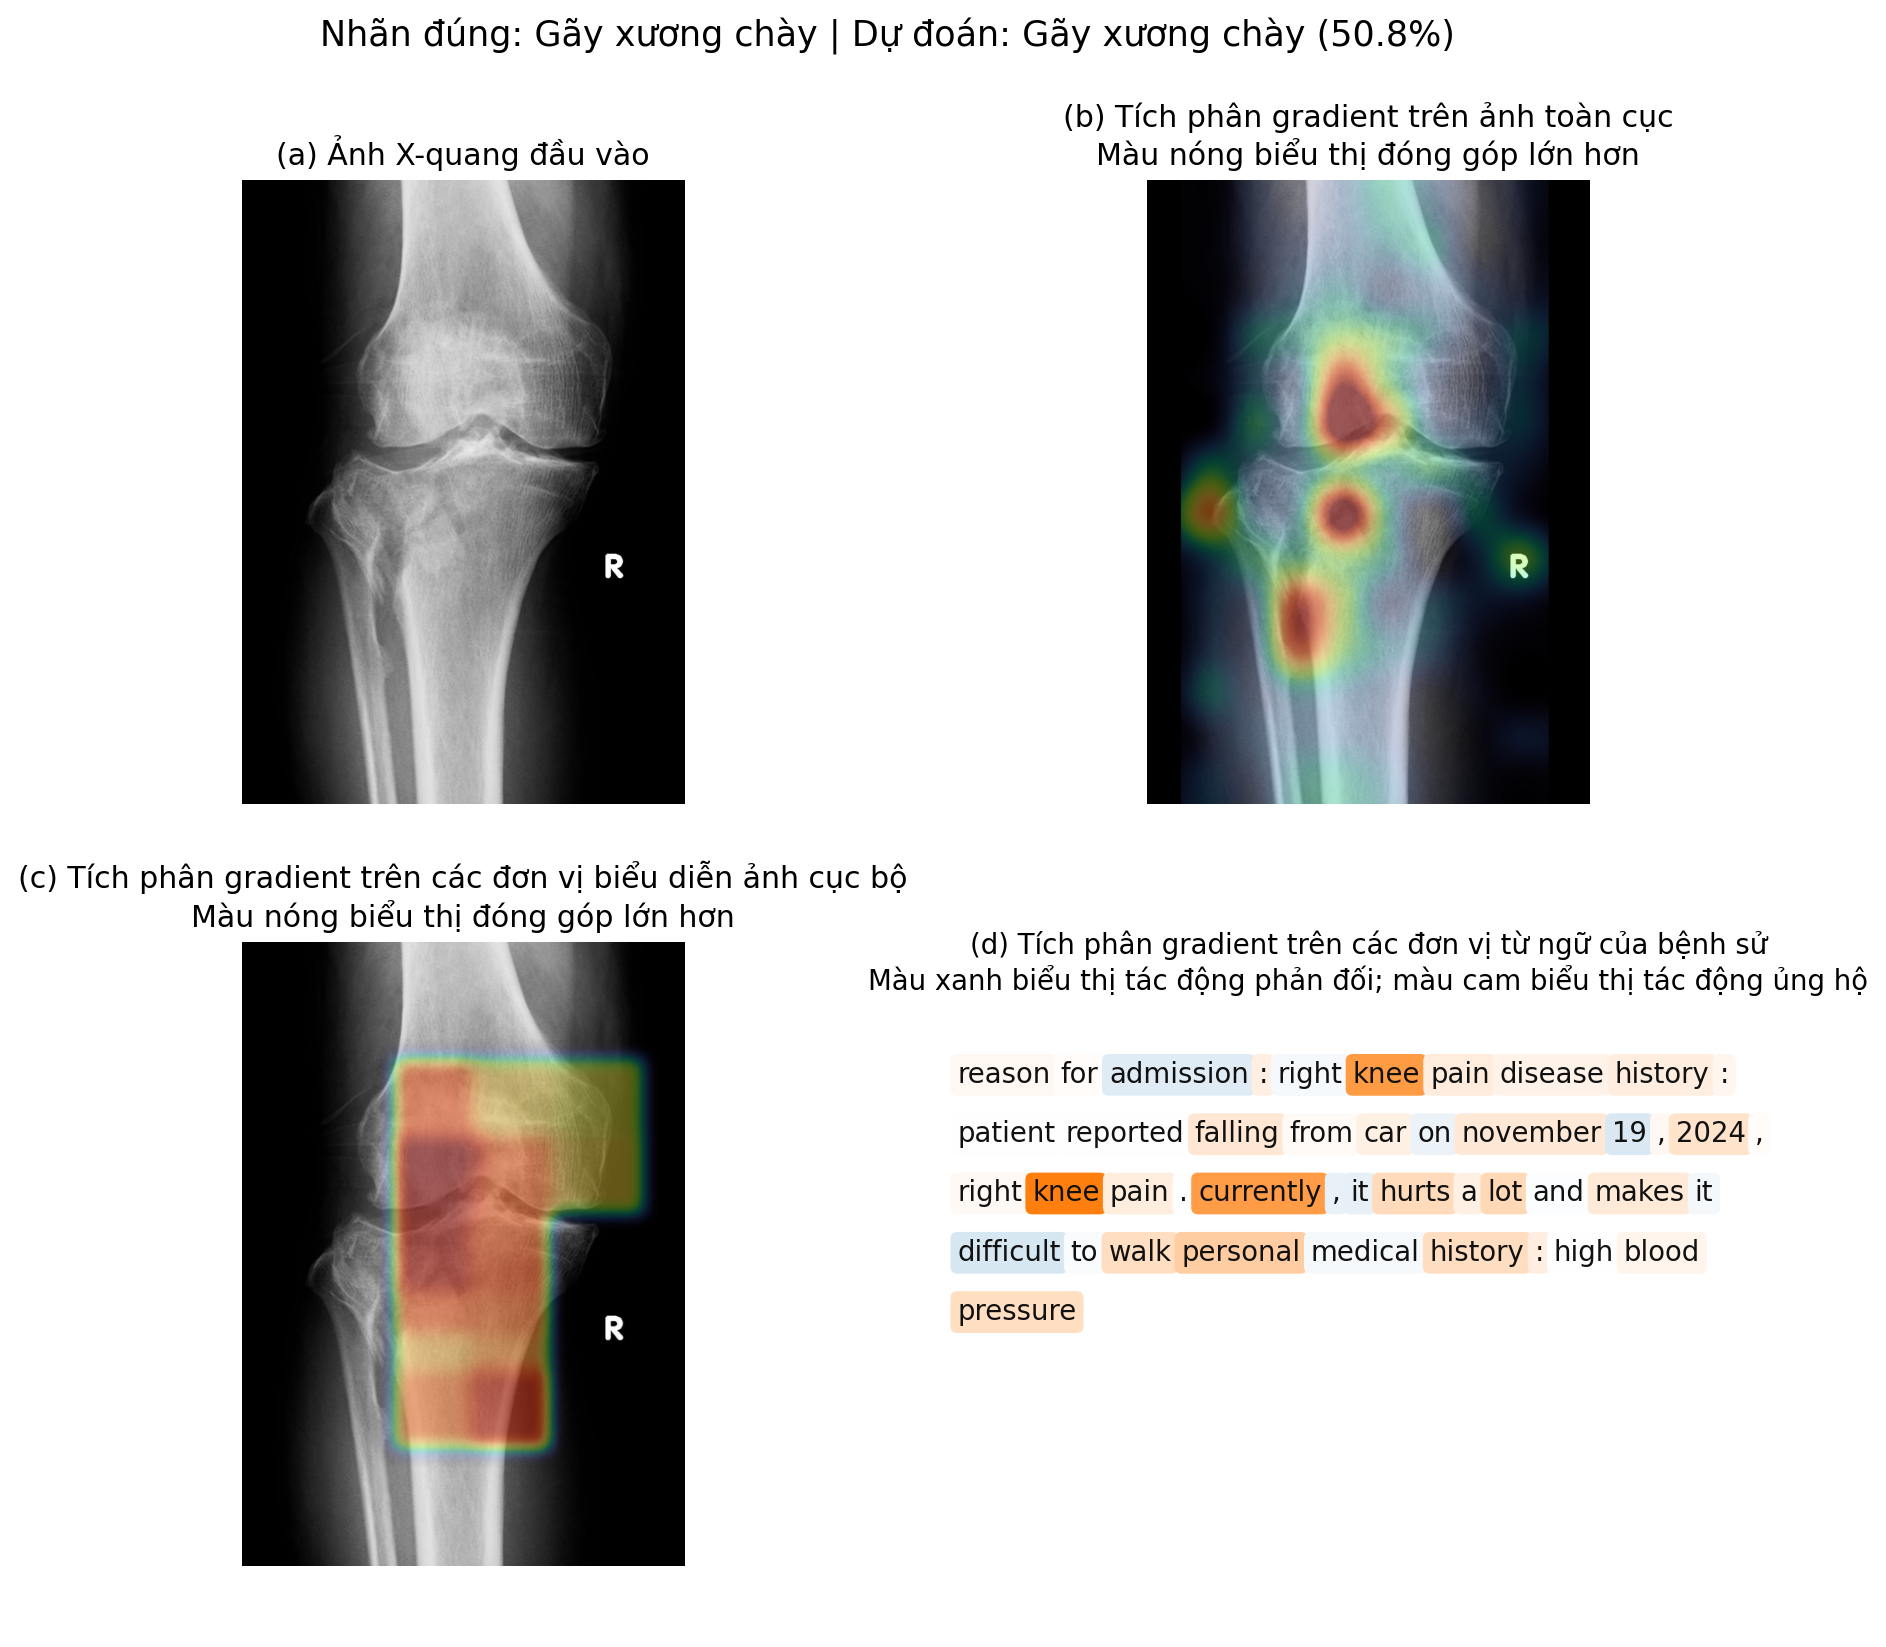
\includegraphics[width=0.85\linewidth]{generated/chapter4_results/multimodal_ig_2842.png}
\caption{Phân tích tích phân gradient của một trường hợp dự đoán đúng gãy xương chày trên CTCH}
\label{fig:explanation_case_correct}
\end{figure}

Hình~\ref{fig:explanation_case_error} trình bày trường hợp có nhãn thật là cắt cụt ngón tay nhưng mô hình dự đoán gãy xương ngón tay với xác suất $71{,}7\%$. Bản đồ ảnh tập trung ở bàn tay và các ngón, trong khi bệnh sử làm nổi bật các cụm mô tả vết thương gần đứt ngón thứ ba và tai nạn do máy. Các nguồn được quy đóng phù hợp về vị trí giải phẫu nhưng không giúp mô hình phân biệt đúng bản chất tổn thương. Trường hợp này cho thấy bản đồ quy đóng có thể hỗ trợ truy vết nguồn mà dự đoán sai liên hệ, nhưng sự phù hợp về vị trí không xác nhận tính đúng của chẩn đoán.

\begin{figure}[H]
\centering
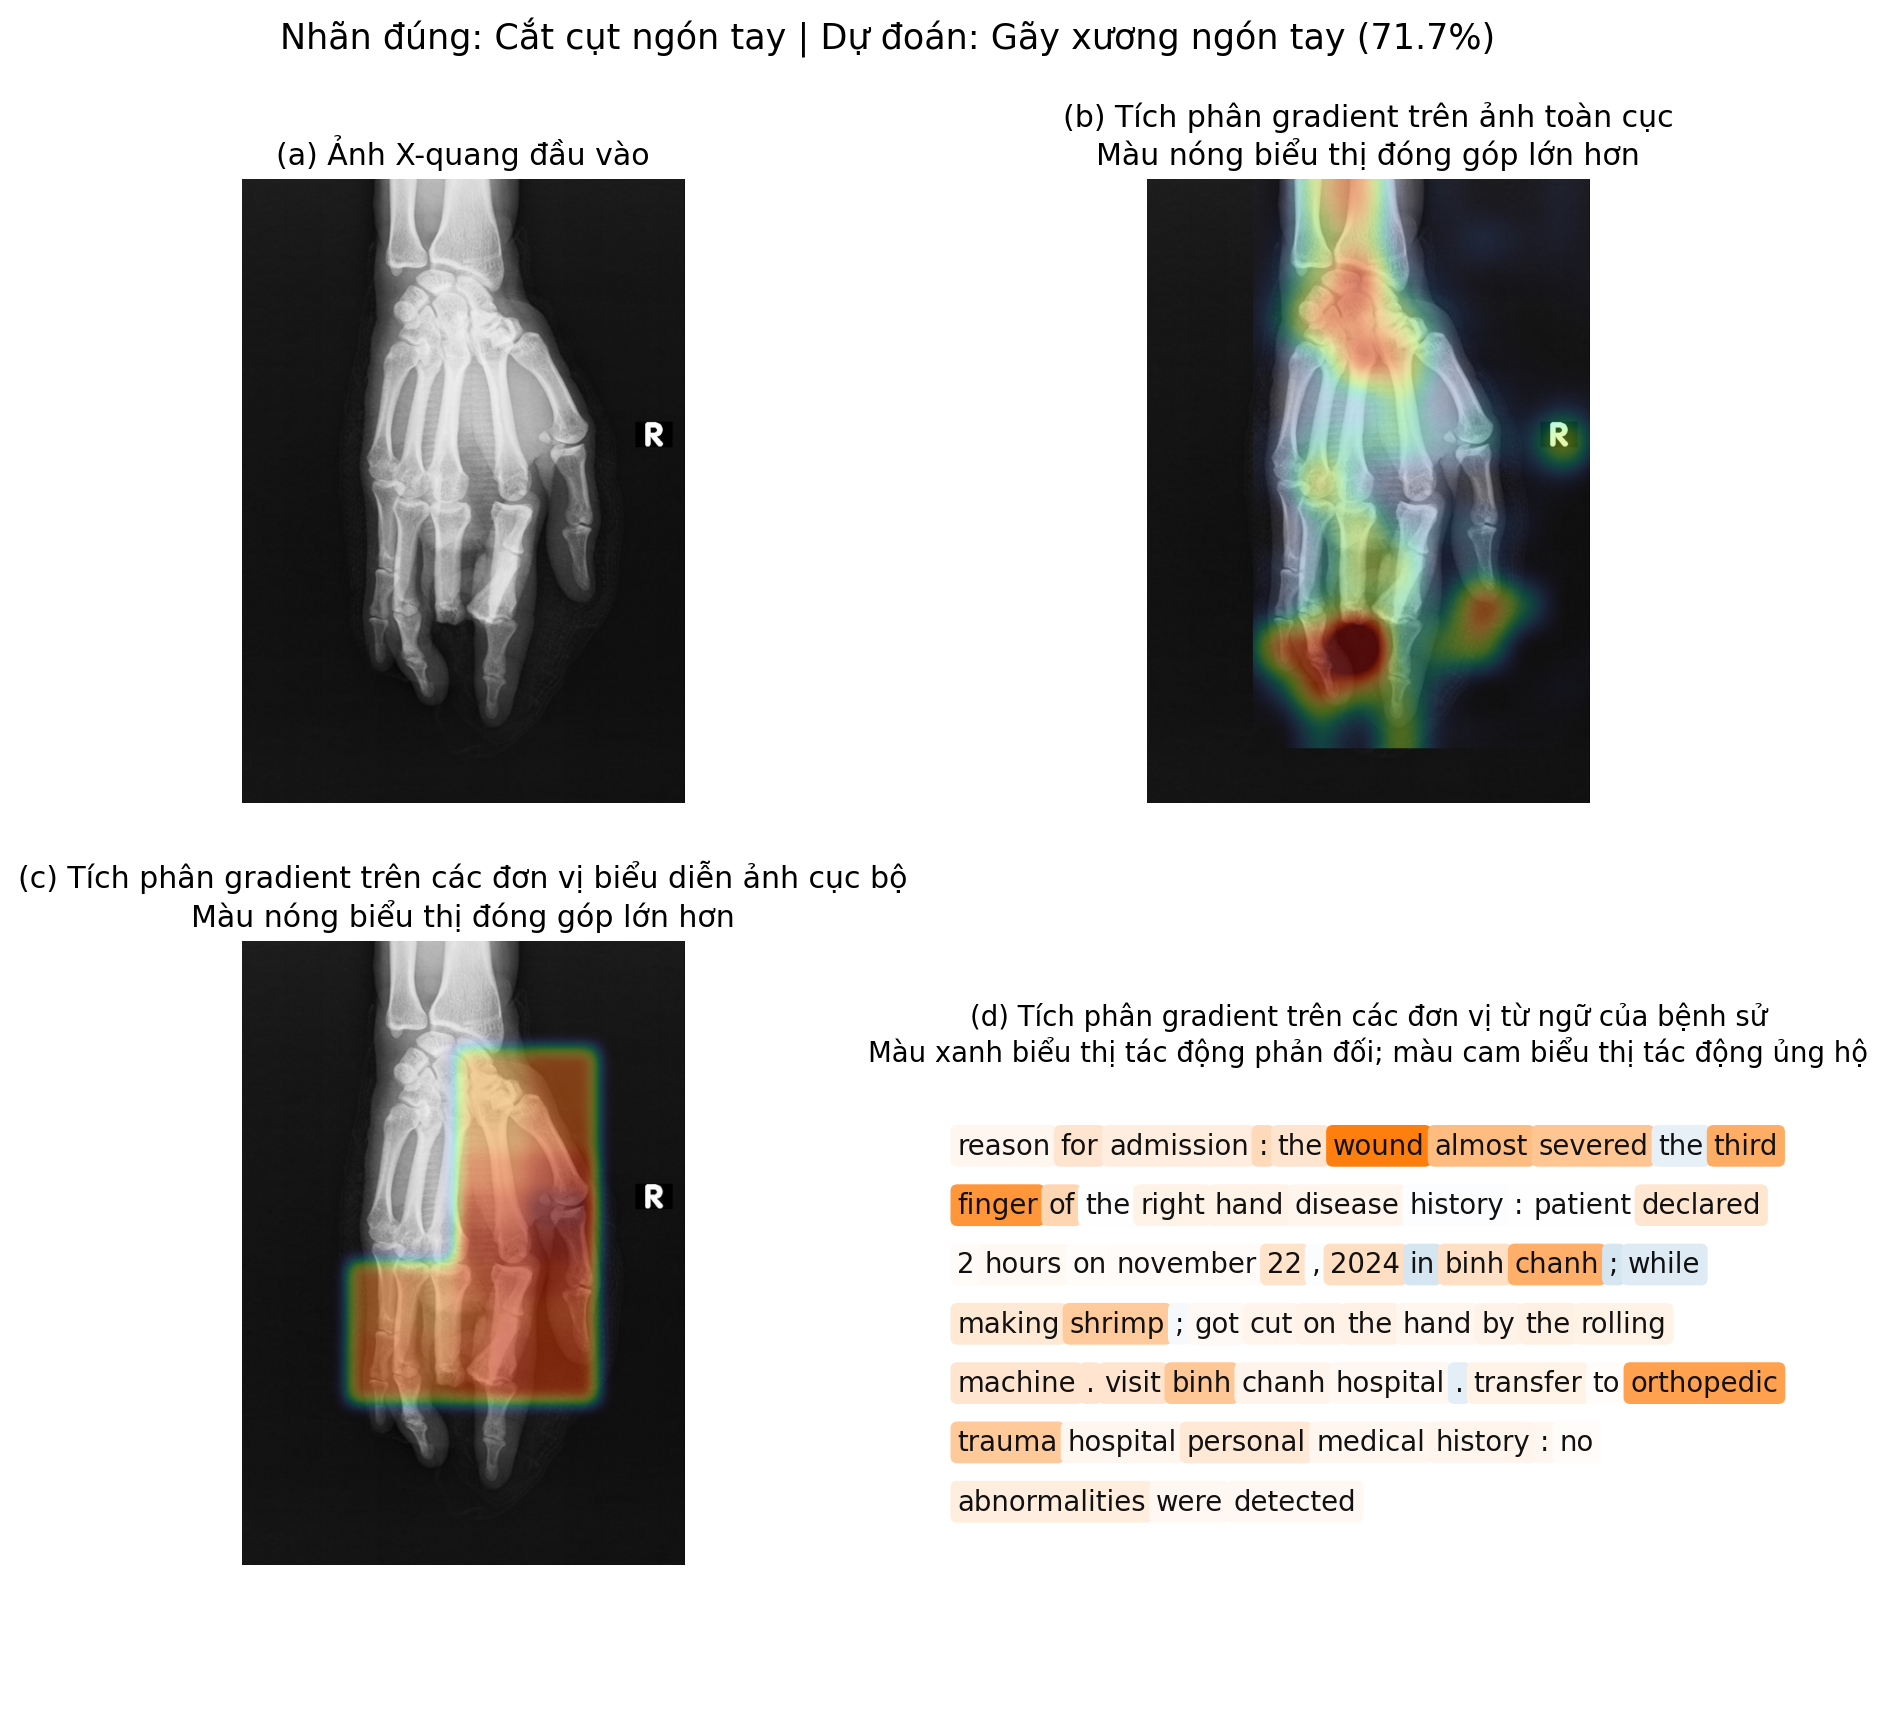
\includegraphics[width=0.85\linewidth]{generated/chapter4_results/multimodal_ig_3021.png}
\caption{Phân tích tích phân gradient của một trường hợp cắt cụt ngón tay bị dự đoán nhầm thành gãy xương ngón tay trên CTCH}
\label{fig:explanation_case_error}
\end{figure}

\subsection{Tổng kết}
Trong phép can thiệp hiện tại, ảnh toàn cục và bệnh sử là hai nguồn tạo mức thay đổi xác suất lớn nhất trên toàn bộ tập kiểm thử, còn ảnh hưởng biên của ảnh cục bộ phụ thuộc mạnh vào mốc thay thế. Thứ tự do tích phân gradient xác định cải thiện AUC loại bỏ so với thứ tự ngẫu nhiên rõ hơn ở ảnh toàn cục và bệnh sử, trong khi chênh lệch ở ảnh cục bộ gần 0. Do đó, bằng chứng về độ trung thực phụ thuộc vào nguồn thông tin và vẫn còn hạn chế. Phân tích định tính làm rõ nguồn phụ thuộc của cả dự đoán đúng và dự đoán sai, nhưng không xác lập quan hệ nhân quả, khả năng định vị tổn thương hoặc độ đúng lâm sàng.
